\documentclass{article}
\usepackage{hyperref}
\usepackage{graphicx}
\usepackage{float}
\usepackage{longtable}
\usepackage{textcomp}
\usepackage{wrapfig}
\usepackage{listings}
\usepackage{pdflscape}
\graphicspath{ {images/} }
\hypersetup{
    colorlinks=true,
    linkcolor=blue,
    filecolor=magenta,      
    urlcolor=blue,
}
\setlength{\parskip}{1em}
\urlstyle{same}
\linespread{1.25}
\begin{document}
\begin{center}
{\Huge An App for Fan Based Live Sports Audio Commentary\\[5cm]}

{\Large Sam Mai

BSc Computer Science

Submission Date: \today

Supervisor: Harry Strange}
\end{center}
\newpage
\begin{center}
{\Large \textbf{Abstract}}
\end{center}
The project involves development of an Android application to provide football fans a social platform to interact with others and motivates users to get involved through live streaming capabilities. The application will be supported by two different servers, one is used for live streaming capabilities and another back-end server to store users' information. The aim of the project is to provide a simple social platorm for Football fans where they can more involved with the sport. The main goal of the project is to develop an Android application that can perform a range of functionalities including: live streaming, live chat and socialising with other users. The main challenge of the project is to ensure the quality of live streams and the experience these live streams will bring to other users.\par
\noindent The project is carried out in an iterative manner, goals and objectives are broken down into smaller objectives that can be achieved in a shorter period of time which in turn would be broken down into a list of weekly objectives. The project involved understandings of different technologies: Android development, PHP scripting + MySQL, Firebase Cloud Messaging and Wowza GoCoder SDK.\par
\noindent The project resulted in a fully functional and tested Android application that achieved the set aims and goals along with a functional back-end server. A document has been produced that provides all technical details about the whole system including a user manual to demonstrate the application's capabilities and a system manual to assist further development.\\
\newpage
Contents
\begin{itemize}
    	\item [1] Introduction \hfill6
	\begin{itemize}
		\item [1.1] The Problem  \hfill6
		\item [1.2] Why I chose this project? \hfill6
		\item [1.3] The Challenges \hfill6
		\item [1.4] Aims and Goals  \hfill7
		\begin{itemize}
			\item [1.4.1] Aims \hfill7
			\item [1.4.2] Goals \hfill7
		\end{itemize}
		\item [1.5] How the project was conducted \hfill8
		\item [1.6] Structure of this report \hfill8
	\end{itemize}
    	\item [2] Background Information \hfill10
	\begin{itemize}
		\item [2.1] Sources of Information \hfill10
		\begin{itemize}
			\item [2.1.1] Android Developers \hfill10
			\item [2.1.2] Android Login and Registration with PHP, MySQL and SQLite \hfill10
			\item [2.1.3] Retrofit - Getting Started and Creating an Android Client \hfill11
			\item [2.1.4] How to Create an Android Chat App Using Firebase \hfill11
			\item [2.1.5] Android Sliding Menu using Navigation Drawer \hfill11
			\item [2.1.6] Stack Overflow \hfill12
		\end{itemize}
		\item [2.2] Similar Products \hfill12
		\item [2.3] Supporting Tools and Libraries \hfill15
		\begin{itemize}
			\item [2.3.1] Retrofit API \hfill15
			\item [2.3.2] Wowza GoCoder SDK \hfill15
			\item [2.3.3] JW Player SDK \hfill16
			\item [2.3.4] Firebase API \hfill16
			\item [2.3.5] The Monkey \hfill17
		\end{itemize}
	\end{itemize}
    	\item [3] Requirements and Analysis \hfill18
	\begin{itemize}
		\item [3.1] Requirements \hfill18
		\item [3.2] Use Cases \hfill19
		\begin{itemize}
			\item [3.2.1] Use Case Diagram \hfill19
		\end{itemize}
		\item [3.3] Entity-Relationship (ER) Diagram \hfill21
	\end{itemize}
	\item [4] Design and Implementation \hfill22
	\begin{itemize}
		\item [4.1] System Architecture \hfill22
		\item [4.2] Data Flow Diagram \hfill23
		\item [4.3] Application Components \hfill24
		\begin{itemize}
			\item [4.3.1] Broadcasting to Streaming Server \hfill225
			\begin{itemize}
				\item [4.3.1.1] Audio Sampling Rate\hfill235
			\end{itemize}
			\item [4.3.2] Database\hfill26
			\begin{itemize}
				\item [4.3.2.1] Structure \hfill26
				\item [4.3.2.2] Implementation \hfill26
			\end{itemize}
			\item [4.3.3] Location Service \hfill27
			\item [4.3.4] Connecting to Server Side \hfill28
			\item [4.3.5] Live Chat \hfill28
			\item [4.3.6] Searching\hfill29
		\end{itemize}
		\item [4.4] Server Components \hfill30
		\begin{itemize}
			\item [4.4.1] Server Database \hfill30
			\begin{itemize}
				\item [4.4.1.1] Structure \hfill30
				\item [4.4.1.2] Implementation \hfill31
			\end{itemize}
			\item [4.4.2] Storing Passwords \hfill31
			\item [4.4.3] POST Requests \hfill32
		\end{itemize}
	\end{itemize}
	\item [5] Testing\hfill34
	\begin{itemize}
		\item [5.1] Stress Testing \hfill34
		\item [5.2] Functional Testing \hfill34
		\item [5.3] Device Testing \hfill35
		\item [5.4] Summary \hfill37
	\end{itemize}
	\item [6] Conclusions and Evaluation \hfill38
	\begin{itemize}
		\item [6.1] Summary of Achievements \hfill38
		\item [6.2] Evaluation \hfill38
		\item [6.3] Future Developments \hfill39
		\item [6.4] Conclusions \hfill39
	\end{itemize}
	\item [7]Appendices \hfill41
	\begin{itemize}
		\item [A] Use Cases \hfill41
		\item [B] System Overview / Class Listing \hfill50
		\item [C] Testing Results \hfill52
		\item [D] System Manual \hfill53
		\item [E] User Manual \hfill54
		\item [F] Project Plan and Interim Report \hfill60
		\item [G] Code Listing \hfill65
		\item [H] References \hfill91
	\end{itemize}
\end{itemize}
\newpage
\begin{flushleft}
{\huge 1. Introduction} \par
{\Large1.1 The Problem} \par
Football is one of the most anticipated sports around the world and due to its popularity, football fans often find it hard to follow every single match in a season for numerous reasons be it travel distance, ticket price, accessibility to content etc. To overcome the problem, people may decide to sit around pubs where they can watch the match or if people have access to a computer, streaming from different sources can also be considered a temporary solution. Of course, these solutions are not perfect and it kills the fun of watching football because of the lack of interactions between the fans which is what football is about.\par
In summary, it's hard for football fans to enjoy the sport they love so much without compromising different important aspects of their lives. Therefore, this project is concerned with providing a social platform for fans who are attending a game to give live audio commentary for other fans to listen to.\par
{\Large 1.2 Why I chose this project?} \par
I chose this project because this is the problem that my family members also experience a lot and it can be quite frustrating to certain people hence needs to be resolved.\par
Apart from that, I also feel that this is the perfect opportunity to learn and improve my technical capability by tackling new areas which I have little to no experience in.\par
Furthermore, not only helping those that don't have frequent access to football matches but the application will also draw people with access to the game by allowing them to socialise with other while giving their thoughts and insights of the game under the form of streaming.\par
{\Large 1.3 The Challenges} \par
1) The first challenge is to ensure that the commentary reflects what's actually happening during the match. It's obviously not possible to ensure every single detail is correct and stream monitoring would cost a lot, not mentioning it's also not technically feasible. However, there are partial solutions to ensure the commentary reports what's actually happening during the match by ensuring the commentator is actually present in the stadium at the time.\par
2) Another challenge is the quality of the audio stream, this is compromised by a lot of factors mainly due to different sample rate supported by different devices and the amount of data used for different sample rate (Keeping in mind this is outside where Wi-Fi is not available so the amount of data is limited).\par
{\Large 1.4 Aims and Goals}\par
{\large 1.4.1 Aims}\par
The aim of the project are:
\vspace{-5mm}
\begin{itemize}
	\item [1.] To learn and develop Android applications incorporating a range of different technologies.
	\item [2.] To learn and develop a simple RESTful web service using PHP and MySQL.
	\item [3.] To gain an understanding of good coding practice and apply it in the project.
\end{itemize}
{\large 1.4.2 Goals}\par
This section outlines the list of goals the system wish to achieve using the knowledge gained from fulfiling the aims of the project.
\vspace{-5mm}
\begin{itemize}
	\item [1.] To allow users to follow football games from others’ points of view through live commentaries.
	\item [2.] To allow users to share their thoughts and insights about football games through live commentaries.
	\item [3.] To allow users to express their views on quality of commentaries from different commentators.
	\item [4.] To offer practices to users who are interested in doing audio commentaries.
	\item [5.] To allow users to interact with each other in a friendly manner
\end{itemize}
{\Large 1.5 How the project was conducted}\par
An iterative approach was followed thorughout the duration of the project. The project is divided into multiple cycles with each lasts for a short period of time ranging from two to three weeks. Firstly, the initial version is a working product with only basic functionalities, then further improvements and extra functionalities are added in every increment leading all the way up until the end of the project as shown in figure \ref{fig:iterative-plan}.\par
\begin{figure}[H]
	\centering
	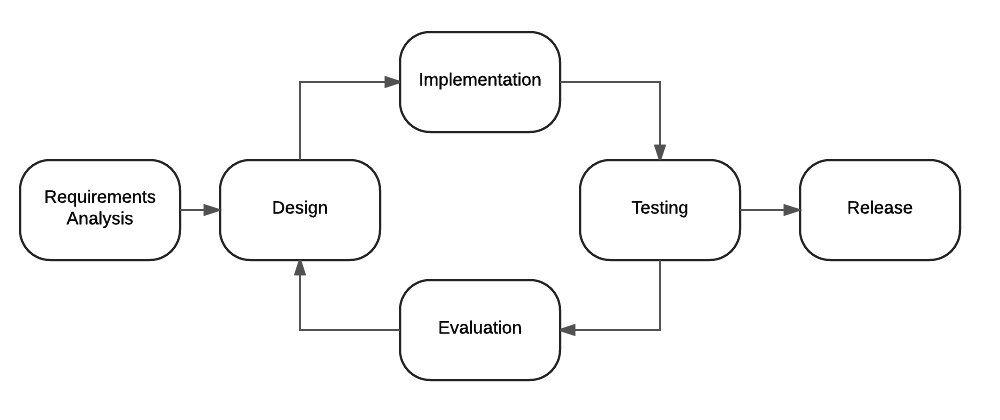
\includegraphics[width=14cm]{iterative-plan}
	\caption{Iterative Approach}
	\label{fig:iterative-plan}
\end{figure}
The project plan highlights the durations for each functionality and different phases of the project. The project plan was later revised in the interim report to make sure everything is going well according to the initial plan and whether there were changes to be made.\par
Meetings with supervisor is also scheduled weekly to report back progress made during the past week, this is also the opportunity to raise any concerns and also ask for feedback for the progression and quality of work. Tasks to be done for the upcoming week will also be discussed here as a collaborative effort.\par
{\Large 1.6 Structure of this report}\par
Following this Introduction chapter, the report will then be followed with 5 more chapters. Chapter 2 will be covering background information and related work. This outlines all the main sources of information of related technologies used during the project. Chapter 3 is Requirements and Analysis which discusses all the work done prior to the implementation period of the project. Chapter 4 covers  all the design and implementation strategies, often there will be more than one of way of implementing a certain functionality, this chapter will also be debating related strategies and weigh up their pros and cons. Next up, chapter 5 will go over all the testing strategies performed and the results. Finally, the final chapter 6 will be the conclusion and evaluation that highlights all notable achievements, also what worked well and what didn't and future improvements to be made to the final product.\par
\newpage
{\huge 2. Background Information}\par
This chapter describes all the background information related to the development of the project and also relevant tools and libraries used. In addition, similar products available in the market have also been mentioned and analysed.\par
{\Large 2.1 Sources of Information}\par
Building a streaming Android application often involves a lot of different technologies and large proportion of time during project was spent on researching about these technologies and their alternatives to find the most suitale product that will fit with the purpose of the project. Details about these technologies will be discussed in the upcoming sections.\par
{\large 2.1.1 Android Developers}\par
Application development in Android is quite complex in comparison to iOS due to the vast variety of products in the market so different screen sizes, solutions, Android versions etc. should be managed well. Furthermore, due to its popularity Android is growing incredibly fast, big codename versions are rolled out every year while small upgrades come out every few months. Android developers\textsuperscript{1} offers a comprehensive guide for Android developers of all levels with frequent updates to help users stay up to date with newer versions of Android. The site also demonstrates best practices for some of the most important aspects such as performance, user input or battery etc.\par
{\large 2.1.2 Android Login and Registration with PHP, MySQL and SQLite\textsuperscript{2}}\par
This guide shows an example of how to add a very basic user authentication functionality with PHP, MySQL and SQLite. The guide is quite user friendly espeically to developers that are new to PHP and MySQL, explanations are provided from beginning to the end including installations of used software. This also demonstrates an overview of how to manage session data using SharedPreferences, in this case it provides a way to manage user log in session. Furthermore, the guide also introduces the use of SQLite database within Android to store personal information such as name, email, etc. This allows the application to access certain information even when device is not connected to the Internet and also reduces delays when requesting for unimportant information, in this case that would be name, email, commentator status etc. In addition, the author also presents very good practices when calling MySQL statements from PHP, more specifically protection against SQL injection. Talking about security, the guide also provides good practice in dealing with user login credentials which is to store the encrypted password and the salt used to encrypt that password instead of the actual password. This way it is harder to actually crack these passwords without knowledge of salting and encryption algorithms used.\par
{\large 2.1.3 Retrofit — Getting Started and Creating an Android Client\textsuperscript{3}}\par
This tutorial aims at providing users a walkthrough on how to use Retrofit - Type-safe HTTP client for Android and Java, from configuring the library to more advanced functionalities such as Pagination etc. This tutorial provides comprehensive steps on making synchronous and asynchronous requests with logging so users can actually see what's being returned from a request call. This tutorial is very straightforward with little to no jargons particularly suitable for new Android developers. Moreover, Android Studio users can conveniently use the library after adding a few dependencies on build gradle. \par
{\large 2.1.4 How to Create an Android Chat App Using Firebase\textsuperscript{4}}\par
This tutorial shows developers how to create a messaging app using Firebase Cloud Messaging (FCM). As Google Cloud Messaging (GCM) is slowly switching over to Firebase, this tutorial is the perfect example of how Firebase is much more versatile than GCM. The tutorial makes the most use of all the new features of FCM including built-in authentications or database even log in and registration UI screens are pre-built. Server side is now optional hence following this tutorial developers can very quickly design their own live chat applications. Furthermore, for Android Studio users the guide also makes use of built-in functionalities that allows developers to connect to Firebase within few clicks.\par
{\large 2.1.5 Android Sliding Menu using Navigation Drawer\textsuperscript{5}}\par
This is a bit of an anomaly in a way that it shows readers how to use Navigation Drawer which is a part of UI design. Unlike other sources of information this tutorial dedicates primarily on UI design and how to interact with different fragments. There are quite many new topics involved in this tutorial that new developers may not be aware of. The tutorial also outlines a number of useful techniques and libraries developers can use to make their applications look more professional.\par
{\large 2.1.6 Stack Overflow\textsuperscript{6}}\par
Stack Overflow is the largest online community where programmers can share knowledge through the form of questions and answers. It is a massive knowledge pool with nearly 1,000,000 questions related to Android development.\par
When developing an Android application, even the most experienced developers make mistakes, these problems can be the most basic as a typo to more advanced performance related problems. The best thing about Stack Overflow is its large community, developers will often find many solutions to a certain problem, advantages and disadvantages are often discussed in details by other developers. This is probably the fastest way for a developer to learn and progress.\par
{\Large 2.2 Similar Products}\par
Below tables outline a range of similar products available on the market at the moment.
\begin{longtable}{| p{2.2cm} | p{9cm} |}
\hline
Name & Mobdro\textsuperscript{7}\\
\hline
Operating System & Android\\
\hline
Description & Mobdro is a tool that constantly looks for free video streams available on the web and makes them accessible on your mobile device.\\
\hline
Advantages & 
\begin{itemize} 
	\item Wide range of videos on diffrent topics.
	\item Sharing recommended videos.
	\item Bookmark favourite channels.
	\item Capture streams.
\end{itemize}\\
\hline
Disadvantages &
\begin{itemize}
	\item Cannot record a stream from the application.
	\item Advertisements on freemium version.
	\item Does not have a live chat room where users can interact.
\end{itemize}\\
\hline
\end{longtable}

\begin{longtable}{| p{2.2cm} | p{9cm} |}
\hline
Name & Ustream\textsuperscript{8}\\
\hline
Operating System & Android\\
\hline
Description & Ustream is a well known streaming application supported by a wide range of devices.\\
\hline
Advantages &
\begin{itemize}
	\item Guaranteed to support a range of devices such as Samsung Note 4, LG Nexus 4 etc.
	\item Watch live videos and discover upcoming events on different topics not just Sports.
	\item Broadcast live video using device's camera.
	\item Ability to follow or bookmark favourite channels.
	\item Interaction with audience via chatting.
\end{itemize}\\
\hline
Disadvantages &
\begin{itemize}
	\item Is not a sport-oriented application.
	\item Lacking capability to broadcast with just audio.
	\item Interaction between users are only viable when streaming live.
	\item Advertisements on freemium version.
\end{itemize}\\
\hline
\end{longtable}

\begin{tabular}{| p{2.2cm} | p{9cm} |}
\hline
Name & UK TVNow\textsuperscript{9}\\
\hline
Operating System & Android\\
\hline
Description & UK TVNow is a tool that provides live TV channels from various countries that covers all major categories like sports, entertainment, movies etc.\\
\hline
Advantages &
\begin{itemize}
	\item Offers live stream TV channels in high quality.
	\item Supposedly works with all Android devices.
\end{itemize}\\
\hline
Disadvantages &
\begin{itemize}
	\item Channel based only so the list of streams will be limited.
	\item Offers no means for interactions between users.
	\item Cannot disable advertisements
	\item Users are not able broadcast own streams.
\end{itemize}\\
\hline
\end{tabular} \par
Overall, \textit{Mobdro} and \textit{Ustream} are formidable competitors with \textit{UK TVNow} lacking behind due to the nature of the application which only supports live TV channels. Based on our aims and goals, \textit{Ustream} has a slight edge over \textit{Mobdro} as the application also supports broadcasting via device's camera. But even \textit{Ustream} lacks certain functionalities like: Broadcasting with just audio or a live chat channel for all users to interact with another (users can only interact via the comment section in a video). This is what our application could offer that other competitors couldn't.\par
{\Large 2.3 Supporting Tools and Libraries}\par
{\large 2.3.1 Retrofit API}\par
Retrofit is a type-safe HTTP client for Android and Java. The library is used extensively in the application as a way to interact with the server side to provide most of the main functionalities like logging in, commenting and such. However, just like most other products, there are competitors to retrofit, most well known one is Volley which is another HTTP library developed by Google.\par
Both libraries have their own advatages and disadvatages over the other, Volley is better in terms of flexibility that it supports more HTTP clients such as legacy Apache, HttpUrlConnection, , Apache-4 or OkHttp while Retrofit only really works with OkHttp. On the other hand, Retrofit offers ease of use as it is a lot easier to configure with slightly boost in terms of performance against Volley. Another reason why Retrofit was preferred over Volley is because Volley has a dependency  to Apache HttpClient on a number of its classes. Apache HttpClient is deprecated on Android since API 23 and Volley has not been migrated to non-deprecated APIs.\par
{\large 2.3.2 Wowza GoCoder SDK}\par
Wowza GoCoder SDK is a developments kit designed specifically for end-to-end mobile live video app development. Wowza GoCoder simplifies app developments and is directly integrated with Wowza Streaming Cloud which is the cloud platform chosen for this application. The GoCoder SDK allows access to advanced features and provides detailed control of video and audio encoder settings including support for video resolution up to 4k Ultra HD. The SDK also includes multiple-camera support , enabling dynamic control of focus, exposure and flashlight.\par
One big advantage of using Wowza GoCoder SDK is its direct integration with Wowza Streaming Cloud. The stream will be published to the cloud via an RTSP push stream which can be easily configured using Wowza GoCoder SDK. This is a big advantage because there are very few ways to record and publish a live stream from Android devices to popular streaming cloud services such as Wowza or Azure Media Services. The first way to do this is using Real-Time Messaging Protocol (RTMP) which is not natively supported by Android, developers will have to implement this protocol from scratch which will take a long time or they can rely on external APIs but most of them are outdated and not well maintained. The other way is to use Real Time Streaming Protocol (RTSP) which is natively supported by Android but again it is not very extensive and not well documented.\par
{\large 2.3.3 JW Player SDK}\par
The JW Player SDK is built on top of Android's native media player frameworks which allows developers to take advantage of the flexibility of the native OS with enhanced features and performance. Apart from the capability for HLS playback, the SDK also supports MPEG-DASH playback with enhanced features such as user-selectable playback quality or 360 Video and VR playback.\par
Although there are a range of media players that can be integrated into the application, including Android native media player or ExoPlayer (\url {http://google.github.io/ExoPlayer/}), JW Player was chosen for a number of reasons. Firstly, its ease of use is definitely a massive advantage over other choices, let's take Android media player for example, configuration is not very straightforward there are multiple things to be taken into account such as SurfaceHolder, SurfaceView etc. Whereas for JW Player this is not the case, it can be as simple as adding a fragment and then pass the URL link to the initialised player. Another reason for choosing JW Player is that it is very well documented with demos that demonstrates good practices using the SDK with a very helpful community. Finally the SDK is also free given its extensive range of features.\par
{\large 2.3.4 Firebase API}\par
The Firebase API helps developers to quickly develop high-quality apps by allowing users access to a number of useful features including: Analytics, Authentication, Cloud Messaging and Realtime Database. Firebase Cloud Messaging (FCM) is the newer version of Google Cloud Messaging (GCM) that inherits GCM's core infrastructure but is simpler and server side development is optional because FCM can be used in conjunction with Firebase realtime database and authentication system.\par
FCM works by calling an instace of Firebase Database and push the message to Firebase server. In order to receive new message sent by other users, the chat activity will be subscribed to the Firebase database hence when new message is sent, other devices will automatically pull this message and display it on the screen.\par
{\large 2.3.5 The Monkey\textsuperscript{18}}\par
The Monkey is a program that runs on emulators or actual Android devices to stress test the application by generating a series of pseudo-random user events including clicks, gestures or even system-level events like turning on/off Bluetooth, Airplane Mode etc. This allows developers to spot errors that usually are hard to trigger.\par
The Monkey came pre-installed along with Android SDK Platform-Tools which are required for Android app development. The Monkey can be launced from the command line and is very flexible such that percentage of different types of events can be controlled or tests can be set to run on only a specific package etc.\par
\newpage
{\huge 3. Requirements and Analysis}\par
In order to achieve a high quality design, there's a need to determine specific feature expectations. This chapter will be discussing the process involved and how the requirements are gathered.\par
{\Large 3.1 Requirements}\par
The basic set of requirements was gathered from the problem statement outlined in the \textit{Introduction} chapter in addtion with the challenges, aims and goals of the project. This was then further expanded by examining similar products available on the market to see what they could and couldn't offer to users. Finally, a few potential users  were surveyed to ensure the requirements meet users' expectations.
\begin{longtable}[t]{| p{1cm} | p{6cm} | p{1.8cm} | p{2cm} | p{1.2cm} |}
\hline
ID & Requirements & Type & Category & Priority \\
\hline
RQ1 & The app shall use the user's username and password for authentication. & Functional & Security & Must\\
\hline
RQ2 & The app shall have 2 different accounts: normal user and commentator. & Functional & Accounts & Must\\
\hline
RQ3 & The app shall allow all users to register new accounts. & Functional & Register & Must\\
\hline
RQ4 & The app shall use user's registered email as login username. & Functional & Register & Must\\
\hline
RQ5 & The app shall allow all accounts to be set a password. & Functional & Register & Must\\
\hline
RQ6 & The app shall allow all users to listen to live audio commentaries & Functional & Streaming & Must\\
\hline
RQ7 & The app shall allow commentators to stream their commentaries. & Functional & Streaming & Must\\
\hline
RQ8 & The app shall allow all users to search for all commentators & Functional & Searching & Must\\
\hline
RQ9 & The app shall allow all users to search for live commentaries based on football team. & Functional & Searching & Must\\
\hline
RQ10 & The app shall allow all users to rate other commentators. & Functional & Profile & Must\\
\hline
RQ11 & The app shall allow all users to interact with each other through a live chat channel & Functional & Interaction & Must\\
\hline
RQ12 & The app shall allow only commentators at specified location to commentate on a specific game. & Functional & Streaming & Must\\
\hline
RQ13 & The app shall allow all users to listen to past commentaries. & Functional & Streaming & Won't\\
\hline
RQ14 & The app shall be written in Java to run on Android. & Non-Functional & Compliance to standards & Must\\
\hline
RQ15 & The app shall log in a client within 5 seconds. & Non-Functional & Performance & Must\\
\hline
RQ16 & The app shall allow a maximum 500 characters comment. & Non-Functional & Profile & Should\\
\hline
RQ17 & The app shall allow all users to view commentators' profiles & Functional & Profile & Should\\
\hline
RQ18 & The app shall allow only users to sort avalaible commentaries by commentators' ratings when searching & Functional & Sorting & Should\\
\hline
\end{longtable}
{\Large 3.2 Use Cases}\par
A use case is a series of actions or events that describes interactions between actors (could be users, other systems etc.) and the system, to achieve an objective. Use cases are very useful for system design because they ensure the sytem's behaviours are consistent. Use cases can also be used in several stages of the development process like testing where use cases can be used to compare theoretical behaviours of the system against real-world behaviours. The full list of use cases will be included in the \textit{Appendix}.\par
{\large 3.2.1 Use Case Diagram}\par
\begin{figure}[H]
    \centering
    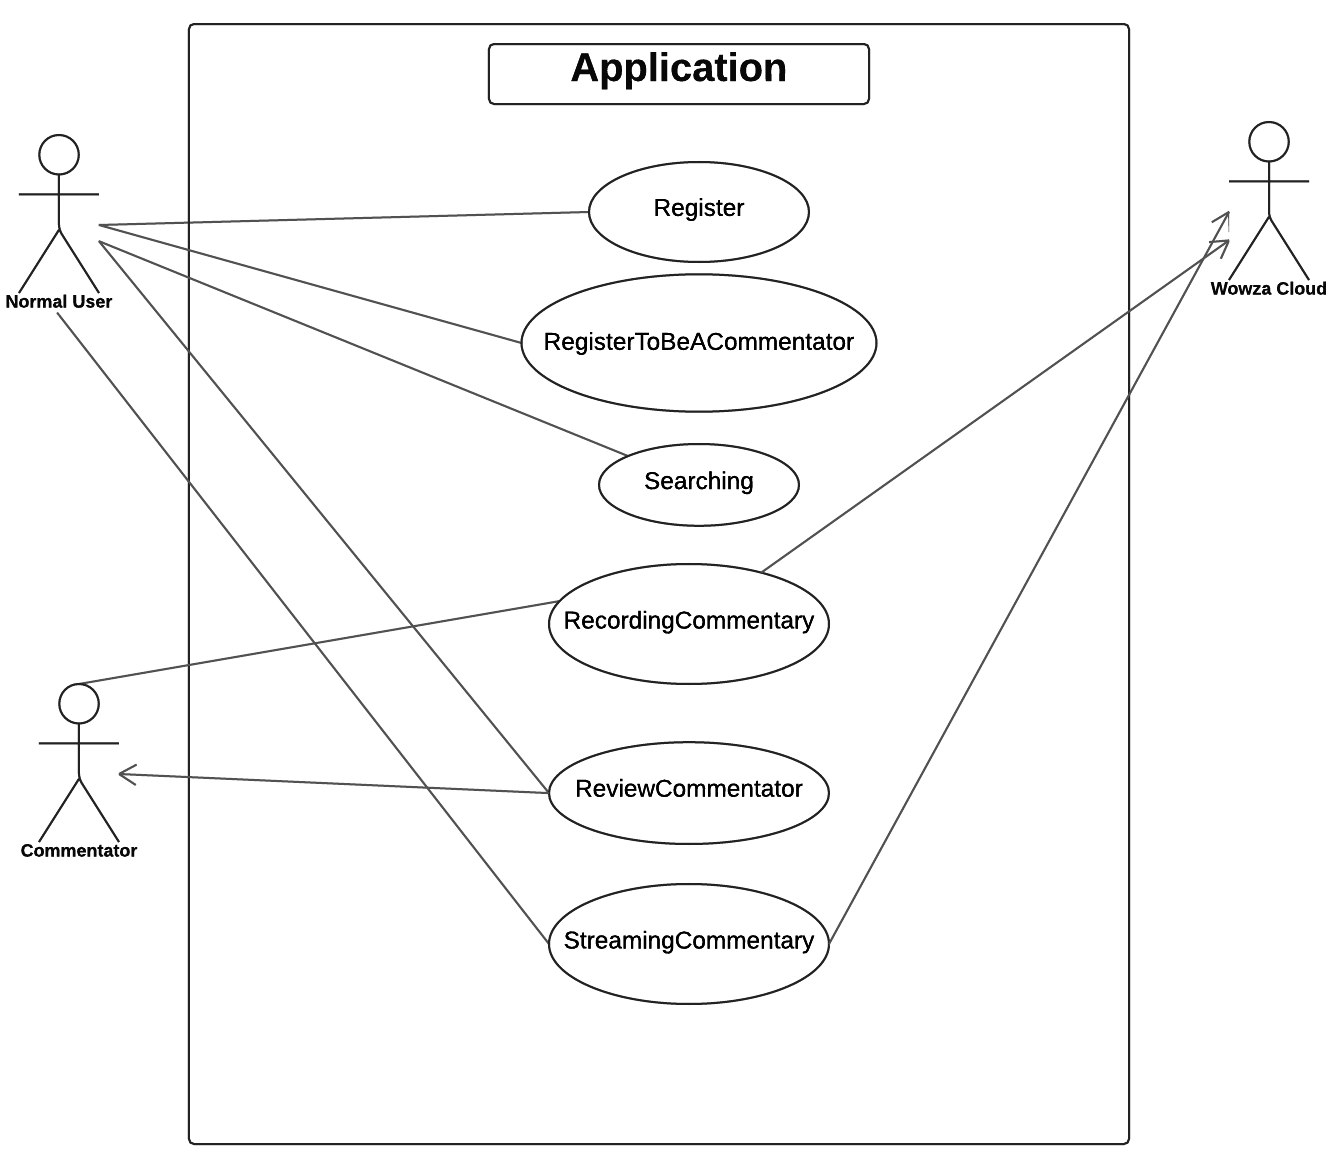
\includegraphics[width=14cm]{use-case-diagram}
    \caption{Application Use Case Diagram}
    \label{fig:use-case-diagram}
\end{figure}
A use case diagram is a graphical representation of use cases that gives an overview of all use cases and actors involved in the system.\par
Figure \ref{fig:use-case-diagram} demonstrates the use case diagram of the application involving three different actors (users or other systems that interact with the subject) that are: Normal user, Commentator and Wowza Cloud. An arrow demonstrates that the actor being pointed to is the secondary actor (indirectly involved) in that particular use case. Likewise, undirected line depicts that the actor is the primary actor (directly involved in the process).\par
{\Large 3.3 Entity-Relationship (ER) Diagram}\par
ER diagrams are graphical representations of entities and their relationship within a system. An entity is an object or concept about which data is stored. A relationship describes how data is shared between two entities.  There are three types of relationships which differs in number of participants involved: one to one, one to many and many to one\textsuperscript{10}. The diagram below will show all the entities involved in the application.\par
\begin{figure}[H]
	\centering
	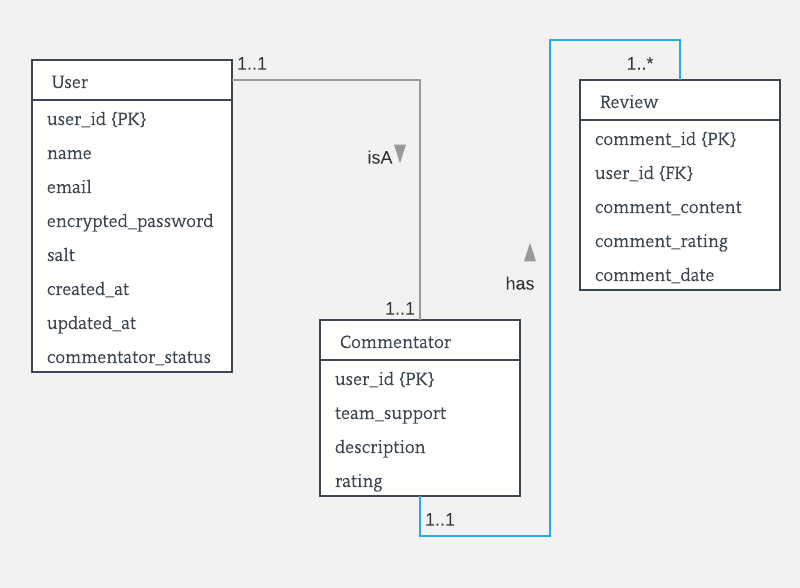
\includegraphics[width=14cm]{er-diagram}
	\caption{Application ER Diagram}
	\label{fig:er-diagram}
\end{figure}
There are three entities involved in a system: \textit{User, Commentator} and \textit{Review}. Typicall, a user can either be a commentator or not and a commentator can have zero or more views.\par
\newpage
{\huge 4. Design and Implementation}\par
This chapter will be describing the overall system architecture and discussing in details certain implementation decisions in comparison to alternatives. There will also be examples of good design practice that have been applied.\par
{\Large 4.1 System Architecture}\par
Similar to other streaming applications, the system is divided into two main components, the back-end webserver and the Android application itself. The back-end webserver handles user-related functionalities that requires interactions with users' data. The Android application component is the front-end that provides graphical user interface (GUI) and links all the functionalities together to provide users a smooth experience.\par
Figure \ref{fig:system-architecture} showcases the overall system. The \textbf{Server Side} is shown on the top of the diagram, it consists of only script files to interact with the database that contains all of users' information. The \textbf{Android Application} component is displayed on the bottom of the diagram that, it shows all of the main activities that are involved with the functionalities displayed in the diagram. The bottom row of each cell demonstrates dependencies and arrows represent the flow of execution of the application.\par
For application part, All classes are quite self-explantory based on their names, not every class is included in the diagram. However, the complete list can be seen in the \textit{Appendix} which also includes the description for each of these activities. Most classes are dependent on server side scripts due to the nature of the application, storing these information in the application database will take up too much space unnecessarily since data are expired quickly so only immutable data such as \textit{user\_id, email} etc. are stored for identity purposes. \par
The complete class listing for server side is also available in the \textit{Appendix}. The main purpose of the server is to provide a mean for application to interact with the database, class \textit{4} to \textit{10} all follow the same model, they encode data returned from database as JSON objects and cut out sensitive information (\textit{password} or \textit{salt} for example) and send that to the applcation. Each of these classes represents a REST call. class \textit{3} is a bit different, it contains all the functions other classes need in order to interact with the database.\par
\begin{figure}[H]
	\centering
	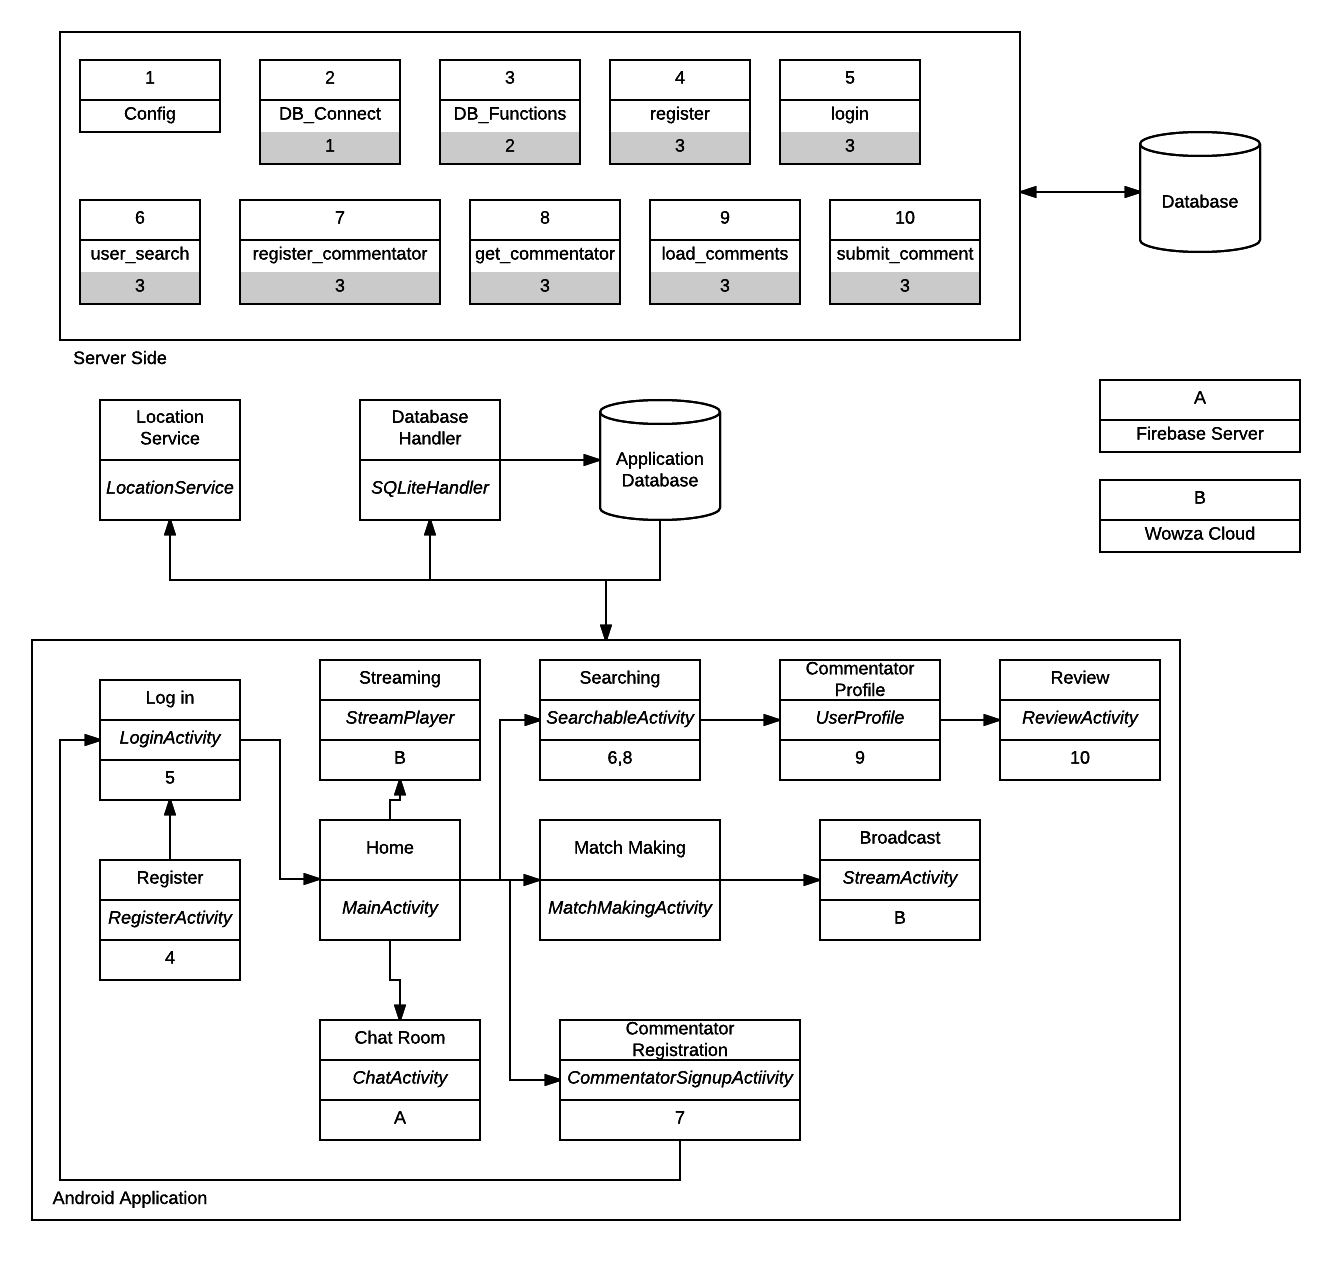
\includegraphics[width=13.5cm]{system-architecture}
	\caption{System Architecture}
	\label{fig:system-architecture}
\end{figure}
Lastly, Firebase Server enables live chat functionality, each time user enters the live chat room, \textit{ChatActivity} will fetch all past comments from this activity and continuallly update it when a new message is sent until the user leaves the chat room.\par
{\Large 4.2 Data Flow Diagram}\par
As the application aims to provide users streaming services, understanding of data flow and different components within the streaming cloud are also quite crucial when designing the system.\par
\begin{figure}[H]
	\centering
	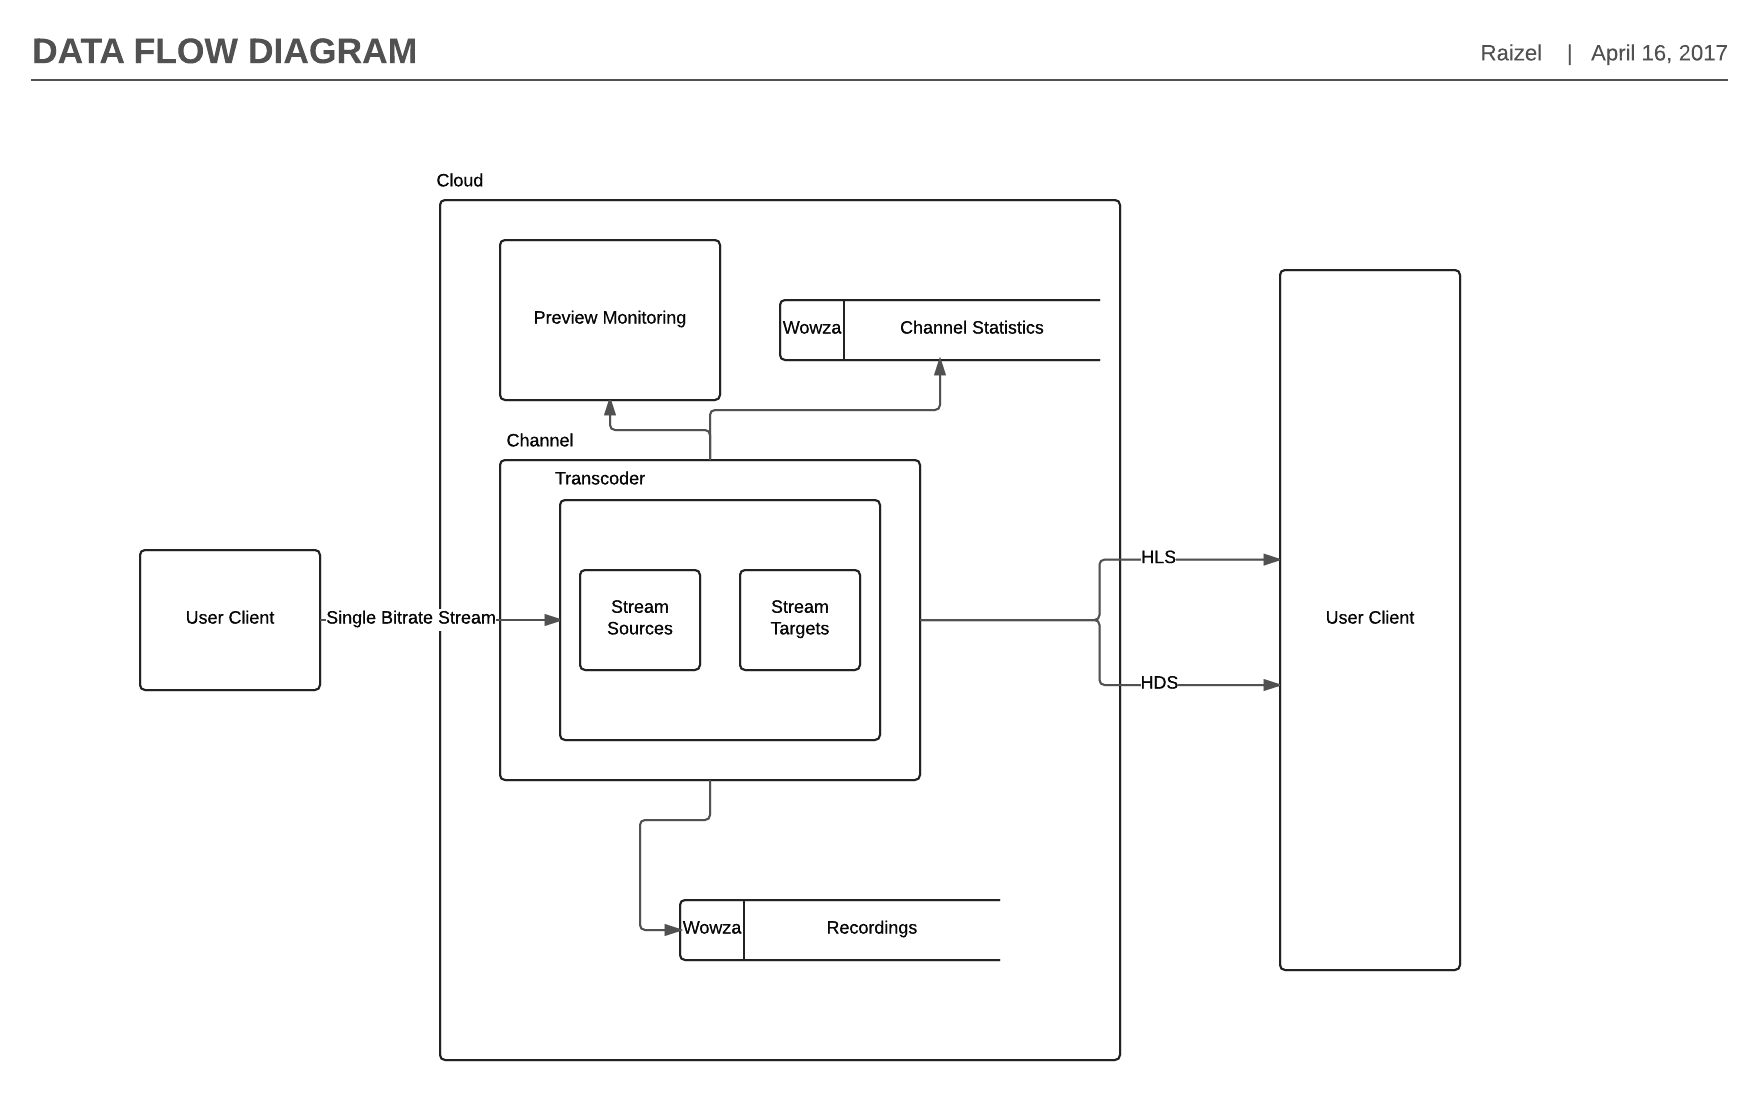
\includegraphics[width=14cm]{data-flow-diagram}
	\caption{Data Flow Diagram}
	\label{fig:data-flow-diagram}
\end{figure}
So the application will send only a single bitrate stream to the channel which can take multiple stream sources at once but can cause congestion. The transcoder is a part of the channel which generates adaptive bitrate passthrough streams and send to specific targets including Facebook Live. This is extended functionality to allow more scalable broadcasts to certain regions or audiences without having geo-blocked channels. Wowza offers two different playback options, Adobe HDS only works with flashplayer which is not supported by Android. Apple HLS is the ideal choice for the system because it is widely supported by a range of different media players available on Android.\par
{\Large 4.3 Application Components}\par
This section will be describing the design of smaller components that make up the Android application.\par
{\large 4.3.1 Broadcasting to Streaming Server}\par
The application relies entirely on Wowza GoCoder SDK to handle the connection to Wowza Streaming Cloud by implementing the \textit{WZStatusCallBack} interface. The workflow is quite simple, it follows a set of procedures to initialise required objects, Below is an overview of the set of functions:
\begin{itemize}
	\item \textbf{initialise()}: This method is self-explanatory, it initialises all required objects. Firstly, it creates a \textit{WowzaGoCoder} (the top level GoCoder API interface) object by giving it a valid Wowza GoCoder SDK key. After that, create an \textit{WZBroadcast} (The broadcaster instance) object along with an \textit{WZBroadcastConfig} (where all credentials to connect to Wowza Streaming Cloud is set, these information are available on user's Wowza Streaming channel) object. Finally an \textit{WZAudioDevice} object that creates an \textit{AudioRecord} instance to record media, which is set to 44.1 kHz sampling rate by default and set to the highest sample rate if the default is not supported, more on this will be available on subsequent section.\\
	\item \textbf{onWZError()}: This method reports any error caused the GoCoder SDK like invalid SDK key.\\
	\item \textbf{onWZStatus()}: This method reports back the status of connection between the device and Wowza Streaming Cloud.\\
\end{itemize} 
\textbf {4.3.1.1 Audio Sampling Rate}\par
Sample rate is the number of samples of audio carried per second measured in Hz or kHz, generally the higher the sample rate the better the quality of audio produced.\textsuperscript{11}. Android's support for audio sample rates varies greatly from device to device and there's also the compromise between size and quality:
\begin{itemize}
	\item 48,000 Hz: Used for DVDs and normally is the maximum sample rate supported by Android devices.\\
	\item 44,100 Hz: The sampling rate of audio CDs which reproduce the maximum frequencies of 20,000 Hz, average humans can't really distinguish frequency above 16,000 Hz and only very small portions can hear above 20,000 Hz. Furthermore, this sample rate is supposed to be the only rate that is guaranteed to work across all devices according to Android documents\textsuperscript{12}. However, even though the sample rate is widely supported, it is not guaranteed to work on every single device i.e. Samsung Note 4 doesn't seem to support it. Another reason for using this sample rate as the default is its size, 10 minutes of streaming at 44100 Hz totalled at around 700 KB or only 7 MB for a full football match, while the output is often 10 times this amount so probably there was some sort of encryption involved in the process.
	\item 22,050 Hz: reasonably popular for low bit rate MP3s,  often used in: AM radio or situations where perceived quality is unimportant but clarity must be maintained.
	\item 11,025 Hz: Very poor sound quality and can be found in WAV files.
	\item 8,000 Hz: Telephone transmission as it is a good trade-off between quality and bandwidth due to limited bandwidth.
\end{itemize}
{\large 4.3.2 Database}\par
{\textbf {4.3.2.1 Structure}}\par
Due to the nature of the application, data is expired quite quickly, so having a confisticated in-app database is unfit in this situation. However, immutable data used to identify the user should still be stored to avoid unnecessary requests to the server.\par
\textit{user}\\
\begin{tabular}{| c | c | c | c | c |}
\hline
uid (PK) & name & email & commentator & created\_at\\
\hline
\end{tabular}\par
These data is used by the application to identify the user, "commentator" column is used to identify the user's commentator status to check if user has rights to broadcast.\par
{\textbf {4.3.2.2 Implementation}}\par
SQLite Database is a library supported by Android, that implements a server-less, zero-configuration SQL engine database. More specifically, SQLite reads and writes directly to disk files hence requires no server and doesn't require installation, while being quite compact at the same time, library can take up as little space as 500 KB with all features enabled. Furthermore, SQLite is cross-platform and so can be copied directly to different platforms\textsuperscript{13}.\par
The application interacts with the database via a helper class named \textit{SQLiteHandler} that extends \textit{SQLiteOpenHelper} an abstract class that manages database creation and version control. This class contains:
\begin{itemize}
	\item \textbf{onCreate()}: The method is called when database is created the first time, \textit{user} table is created in this method.
	\item \textbf{onUpdate()}: typically used for version control, when there's a change to the structure of the table, old \textit{user} table is dropped and it calls \textbf{onCreate()} method to create the new table.
	\item \textbf{addUser()}: Quite self-explanatory, this method is used to store user details in the database, the method is called every time the user logs in.
	\item \textbf{getUserDetails()}: Fetch user details from the database into a hashmap object and return it.
	\item \textbf{deleteUsers()}: this method calls \textbf{getWritableDatabase()} and delete all entries in the table. This method will be called every time user logs out, so at any instance of time, at max only one user is stored in the database, this helps to simplify system while preventing user details from getting stolen.
\end{itemize}
{\large 4.3.3 Location Service}\par
The application uses users' locations to determine whether the user is actually winthin the radius of the stadium when preparing to broadcast. More specifically, users should be within 200 meters (Emirates Stadium is around 17 acres, so this is a reasonable threshold) of the stadium. This is put into place as a measure to prevent users from broadcasting irrelevant contents. Since this is the only purpose of getting users' locations, the application will only check this once because listening to location changes is an intensive process and will waste a lot of battery taking in mind, users will also be broadcasting at the same time. The \textit{LocationService} gets users' whereabouts by implementing \textit{LocationListener} interface that is used for receiving notifications from \textit{LocationManager} when location has changed.\par
On Android, there are two location providers: GPS and Network, each has its own good and bad points.\par
\begin{itemize}
	\item GPS: more accurate but only works outdoors and doesn't respond very fast while consuming more battery.
	\item Network: Determines locations using cellular and wifi signals so it's not as accurate GPS but responds faster, works both indoors and outdoors and also doesn't consume as much battery.
\end{itemize}
The application makes use of both providers, since both speed and accuracy are wanted but not essential. The \textit{getLastBestLocation()} get both locations and compare their times, the newer one is returned.\par
{\large 4.3.4 Connecting to Server Side}\par
The application uses Retrofit to manage transactions between device and the server side which is used thoughout the application, typically functionalities that required interactions with the server side database. Each Retrofit instace is created by caling the \textit{ServiceGenerator} class, the \textit{Datanase} interface is created to contain all the model POST requests (parameters they take, lniks to scripts they call etc.). Retrofit allows both asynchronous and synchronous requests, but since synchronous calls are executed on the main thread therefore UI blocks during request execution reduces application's reponsiveness so in the application all requests are asynchronous. Whether asynchronous and synchronous, they both follow a certain procedure, for our application, a \textit{Database} instance is created by calling \textit{ServiceGenerator} to create a Retrofit instance and call \textit{create(Database.class)} on that instance. After that, the application simply calls the required method from the interface and call \textit{enqueue} to make a request on background thread. In order to get the response, the application simple calls \textit{response.body()} on \textit{onResponse()} method if the request is successful or handle the error on \textit{onFailure()} in case the request was unsuccessful.\par
{\large 4.3.5 Live Chat}\par
The application implements a group live chat as a way for users to interact and socialise with each other. The application uses of the Firebase Cloud Messaging, which is a newer version of Google Cloud Messaging that doesn't require a server side client. Since Firebase API is integrated to Android Studio, new developers will need to spend at most 10 minutes to set up if they got a Firebase account\textsuperscript{4}. So the application takes advantage of Firebase Realtime Database that is pre-configured before hand. The workflow is quite simple:\par
\begin{itemize}
	\item \textit{displayMessages()}: The method populates the view by using \textit{FirebaseListAdapter} class that takes multiple parameters including the layout , the \textit{ChatMessage} class that represents a message object containing: user's name, message content and sent date and lastly a reference to the Firebase Database by calling \textit{FirebaseDatabase.getInstance().getReference()} which gets the root node where all chat messages are stored. Finally, the application will set this adapter on the list view.
	\item Sending message to the database uses the same method \textit{FirebaseDatabase.getInstance().getReference().push().setValue(new ChatMessage())}, where \textit{ChatMessage} is the class made to represent a message object, in this case it takes 2 parameters: name and message content.\\
\end{itemize}
{\large 4.3.6 Searching}\par
The application gives users ability to be able to search for commentators and view their profile. Adding searching functionality on Android\textsuperscript{16} is quite straightforward, adding the \textit{SearchView} to the \textit{App Bar} (The horizontal bar on top of screen) is the first step, next would be adding a \textit{Searchable Configuration} that defines how \textit{SearchView} will behave. Finally, a \textit{SearchableActivity} is created to handle the search query and display results. A more detailed look on the \textit{SearchableActivity}:
\begin{itemize}
	\item \textit{onNewIntent()}: This method is called whenever user performs a search while keeping the activity at the top of the activity stack without launching a new instance, with new \textit{Intent}\textsuperscript{17}. The method sets the new \textit{Intent} for the activity.
	\item \textit{handleIntent()}: Retrieve general action to be performed from the \textit{Intent}, if it's searching then pass the query to \textit{doMySearch()} method.
	\item \textit{doMySearch()}: This method sends a POST request to \textit{user\_search.php} on server to get a list of commentators with relevevant name then populate the view using an \textit{ArrayAdapter}.\\
	\item \textit{getCommentatorProfile()}: This method triggers when users press on any name being displayed, that sends a POST request to \textit{get\_commentator.php} to get relevevant information like rating, description etc. This could be also be performed when transitioned to profile activity instead but that would make the application seems sluggish having sending few POST requests (waiting for a response from server is the main issue here).
\end{itemize}
{\Large 4.4 Server Components}\par
This section will be discussing in details certain aspects of the server side of the system.\par
{\large 4.4.1 Server Database}\par
{\textbf 4.4.1.1 Structure}\par
Database normalisation has been performed to reduce data redundancy and improve data integrity to minimise potential errors occurs when inserting, updating or deleting data.\par
\begin{itemize}
	\item \textbf{1st Normal Form}: Database contains only atomic values and there are no repeating groups\textsuperscript{14}.
	\item \textbf{2nd Normal Form}: To satisfy this, database must be in first normal form and all non-key attributes are dependent on the primary key.
	\item \textbf{3rd Normal Form}: Database is in second normal form and there are no transistive functional dependency i.e. an attribute is dependent on another non-primary key attribute which in turns is dependent on the primary key.
\end{itemize}
\textit{users}
\begin{tabular}{| c | c | c | c | c | c | c |}
\hline
user\_id (PK) & name & email & commentator\_status & encrypted\_password & salt & created\_at\\
\hline
\end{tabular}
\textit{commentators}\\
\begin{tabular}{| c | c | c | c |}
\hline
user\_id (PK) & team\_support & description & rating\\
\hline
\end{tabular}\\
\textit{comments}
\begin{tabular}{| c | c | c | c | c |}
\hline
comment\_id (PK) & user\_id (FK) & comment\_content & comment\_rating & comment\_date\\
\hline
\end{tabular}\par
\textbf {4.4.1.2 Implementation}\par
All interactions with the database use prepared statements\textsuperscript{15} which are very useful against SQL injections. The prepared works as follows:
\begin{itemize}
	\item \textit{prepare()}: Create an SQL statement template without specified values which is sent to the database for syntax checks and initialises resources for later use.
	\item \textit{execute()}: The client binds parameter values using \textit{bind\_param()} and calls \textit{execute()} to send it to the database (since values are sent seperately from query, it cannot interfere with the query which prevents SQL injections) which will create a statement from the template with bound values and execute it.
\end{itemize}
There are multiple benefits for using prepared statements besides the fact that they are useful against SQL injections. Firstly, these statements can be executed repeatedly with different values by changing the bound variable. Another benefit is that it cuts out parsing and validation which makes it runs faster.\par
{\large 4.4.2 Storing Passwords}\par
Security has always been a big issue in application development, storing passwords in plain text is definitely one of worst practices. The system implemented a number of different techniques to prevent passwords from getting stolen in case anyone has access to the database. The process works as follows:
\begin{itemize}
	\item 1: Use PHP \textit{sha1()} hashing function on a random number and take the first 10 characters of that random hash (A hash function is a function that is used to map data of arbitrary size to data of fixed size, pretty much a one way process as it is almost impossible to reverse the hashes back to the original keys). This will be the \textbf{salt} value, a common practice in cryptography to improve complexity. \textit{Note: SHA\-1 is pretty outdated and not recommended for storing passwords, however it is designed to be very fast and efficient which is useful for testing purposes, future developers can quite easily swap it out and use something like SHA\-256 or SHA\-512 instead.}
	\item 2: the \textbf{salt} value will then be concatenated to the password which is then hashed again. The \textbf{salt} will then be concatenated to the outcome once more and the whole thing will be encrypted using \textit{base64\_encode()} function.
\end{itemize}
{\large 4.4.3 POST requests}\par
POST requests are the only way for the application to interact with server side, so there needs to be a consistent way of sending and receiving information and also making sure these data conform to the standard. The system does this by separating the two main components: \textit{DB\_Functions.php} that handles all the SQL statements and a set of scripts that receive what the database return and reformat these data so the application can actually parse it.\par
\begin{figure}[H]
	\centering
	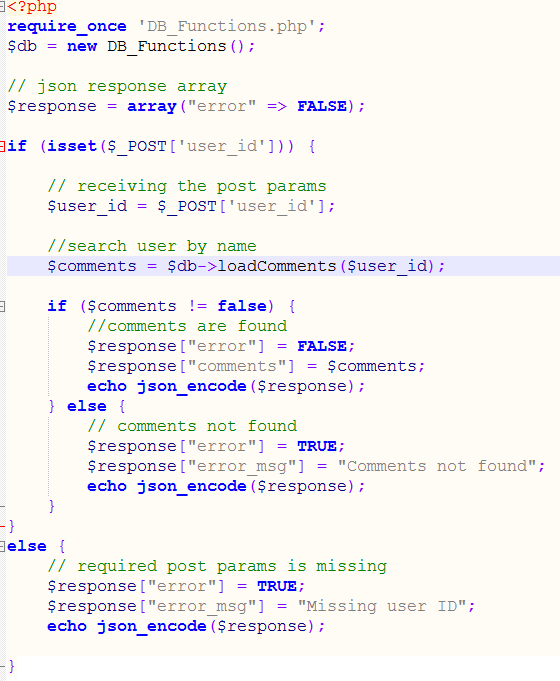
\includegraphics[height=10cm]{load-comments}
	\caption{load-comments.php}
	\label{fig:load-comments}
\end{figure}
Figure \ref{fig:load-comments} shows an example from the load\-comments.php script. It works by checking whether the post request contain \textit{user\_id} field, if not it will set the \textit{error} field to true and return the error message as a json, the application is set to first check the \textit{error} value when receiving a feedback from the server and act accordingly. In other case, if \textit{user\_id} is set, then it will call the function \textit{loadComments()} from \textit{DB\_Functions()} class to send the SQL statement to the database and if it returns false that means no comments has been made about that commentator (it could also mean that the \textit{user\_id} is incorrect, however this function only triggers when an user views a commentator's profile so unlikely to happen) and returns all comments if found any. Like the previous response, it will set \textit{error} value accordingly to the results and return it as a json. All other functionalities like log in or registration follow the same layout structure and principles.\par
\newpage
{\huge Chapter 5: Testing}\par
This chapter will be talking about different types of testing the system underwent and their results.\par
{\Large 5.1 Stress Testing}\par
The Monkey has been mentioned in \textit{section 2.3.5} and is the tool used for stress testing the application. The Monkey was repeated four times on different activities as transitions between activities are also a part of stream of events. Each run consists of 2000 pseudo-random events which adds up 8000 events in total, the results are available in the \textit{Appendix}. The full log will be recorded in a text file which will then be studied carefully for any error occurred duing the run (The Monkey can be set to ignore certain errors and continue running until the count it reached).\par
Out of the four runs, two errors occurred, an interesting one found was a \textit{NullPointerException} on \textit{RegisterActivity}. This happened as a result of multiple requests sent to the server at once which rendered it unresponsive and when the application finally receive a  the application tries to parse the feedback from the server which was supposed to be a JSON object like the normal workflow. However, the server couldn't cope with this many requests at once (the server is hosted on \textit{000webhost} on a free account so performance is relatively bad), at one instance the server returned nothing hence the reason the error occurred, followed by many \textit{SocketTimeoutException} messages which means the request failed and that would follow a different workflow. In reality, this is highly unlikely to happen since the application will display a \textit{ProgressDialog} when waiting for a response from the server which means users won't be able to resubmit the query multiple times. As for the server side, in situations where request can reach the server, application will definitely receive a JSON response, so it was rather interesting to see the server returned nothing at all (even if request couldn't reach the server, application may not receive a JSON but some other response which will result in another error \textit{JSONException} that normally won't disrupt the workflow of application since it's handled).\par
{\Large 5.2 Functional Testing}\par
Test cases were devised from the list of MoSCoW requirements to ensure all the implemented functionalities are working flawlessly. In addition to that, some test cases also look at activity transitions to analyse application's behaviours. Overall, coverage was 100\% for all implemented requirements (RQ9 and RQ18 have not been implemented due to budget problems, Wowza Streaming Cloud only allows paid users to have access to REST API which can be used to dynamically control the cloud from other devices i.e. create channels, get all running channels etc.)\par
The full summary can be in the \textit{Appendix} section, one particularly interesting case was TC8 where a comment recently submitted by a user is not shown under the the commentator's profile when user is directed back to the commentator's proffile. This doesn't however indicate the comment hasn't been added because user will only be directed back to commentator's profile page if the comment has been added successfully. The problem lies in the way how the application transits between the two activities. When the application has confirmed that the comment has been added successfully, it calls \textit{finish()} which in subsequent triggers \textit{onDestroy()} method, now the application redirects users back to the activity before it that is the commentator's profile page. This is the expected behaviour, but the \textit{UserProfile} activity is also expected to be restarted. The fix is rather simple, so now instead of calling \textit{finish()} the application will simply call \textit{startActivity} instead to update the comments.\par
{\Large 5.3 Device Testing}\par
The application has been tested on a number of physical devices of different sizes and Android versions:\par
\noindent \textbf{Device}: Samsung Note 4\hfill \textbf{Device}: OnePlus One\\
\noindent \textbf{Android Version}: 6.0.1\hfill \textbf{Android Version}: 5.1.1\par
\textbf{Device}: Motorola Moto G\\
\textbf{Android Version}: 5.1\par
Testing against these devices kinda gives an idea how well the application copes with different sreen sizes and Android versions. As a result, the app performs normally on all three devices, except there was a problem with recording on the Note 4. Wowza GoCoder SDK doesn't seem to have a suitable profile set for Note 4, even when using \textit{AudioRecord}\textsuperscript{12} class manually without the intervention of GoCoder SDK. The application cycled through a list of standard sample rates from 8,000 Hz up to 96,000 Hz but still unable to find the correct profile, interesting thing is even camera view doesn't seem to be working. This doesn't seem to be related to the hardware side of things because native apps pre-installed on the device using camera and mic still work. There were a few suggestions leaning towards the new 6.0 Android version being more secured \url{http://stackoverflow.com/questions/27878458/android-audiorecord-troubles} and extra permissions needed to be supplied. However, this method still doesn't work, for the time being only other 2 devices are confirmed to be working with broadcasting functionality.\par
\begin{longtable}{| l | l |}
\hline
Sample Rate	&  Sample Size (10 minutes)\\
\hline
8000 MONO &	4.68MB\\
\hline
16000 MONO &	9.24MB\\
\hline
22050 MONO & 13.06MB\\
\hline
32000 MONO &	17.60MB\\
\hline
44100 MONO &	25.40MB\\
\hline
48000 MONO &	27.20MB\\
\hline
8000 STEREO &	9.20MB\\
\hline
16000 STEREO & 18.60MB\\
\hline
22050 STEREO & 24.80MB\\
\hline
32000 STEREO & 37.40MB\\
\hline
44100 STEREO & 50.60MB\\
\hline
48000 STEREO & 55.60MB\\
\hline
\end{longtable}
The table above shows the sample rate and channel configuration of the recording device and its corresponding size that has been performed as a part of an experiment to find the suitable configurations for broadcasting. The experiment was performed on the \textbf{Motorola Moto G}, the sample size represents raw audio data so this isn't necessarily how much data will be used in audio broadcasting. Also methodology for recording on STEREO was quite wrong, since data should be seperated and read pairwise (so [1],[2] to left channel, [3][4] to right channel etc.) so effectively they should be the same size for a given sample rate. Overall, 48000 Hz and 44100 Hz offer the most clear sound and the difference between them are unnoticeable, so in the end the application used 44100 Hz MONO as the default configuration (STEREO is not supported by some devices while MONO is guaranteed to work).\par
{\Large 5.4 Summary}\par
Overall, a wide range of tests have been performed both during and after development period which provides the confidence that the application has met its requirements. Over time, as functionalities grow, more and more tests can be added to the test suite that can keep all functionalities in check and make sure that newly implemented functionalities don't break the old code.\par
\newpage
{\huge Chapter 6: Conclusions and Evaluation}\par
{\Large 6.1 Summary of Achievements}\par
The project has managed to achieve its aims and goals set in section 1.4, more specifically:
\begin{itemize}
	\item To allow users to follow football games from others' points of view through live commentaries: All registered users users are able to listen to live stream freely without any limitation.
	\item To allow users to share their thoughts and insights about football games through live commentaries: As long as users have registered to become commentators, they are allow to broadcast when statationed within 200 metres radius of the stadium. Due to budget limitation, end users cannot directly control Wowza Streaming Cloud because a paid account is required to use the REST API, so currently channel address is hardcoded and requires account owner to start the channel manually.
	\item To allow users to express their views on quality of commentaries from different commentators: This is expressed under the form of rating and reviewing commentators. All users have the freedom to cast a vote and share their opinions about other commentators which would appear under the commentators' profiles.
	\item To offer practices to users who are interested in doing audio commentaries: No qualifications or experience are required for an user to become a commentator, it's a simple process that can take literally 2 minutes and user is ready to broadcast.
	\item To allow users to interact with each other in a friendly manner: An FCM based live chat channel is available 24/7 for users to interact with other users with no additional requirements imposed.
\end{itemize}
{\Large 6.2 Evaluation}\par
In terms of completeness of the project judging from requirements list on section 3.1, the project managed to to complete 83.3\% of these requirements with the exceptions RQ9 and RQ18 due to budget limitation so automation of streaming channels couldn't be achieved. The last requirement that hasn't been achieved is RQ13, a "Won't have" requirement which had been agreed to be included in future releases instead of the initial release.\par
Over the course of development period, a number of good design and implementation practice has been followed. Let's take how passwords are stored in section 4.4.2 for example, a combination of different techniques is used: passwords are hashed and encrypted multiple times reduces the chance of passwords getting stolen. Another example could be the way the server sends queries to the database as described in section 4.4.1.2, the system follows good practice of using prepared statements to guard against SQL injections. It is also quite noticeable that the end of development period produced more cohesive and well-structured code in comparison to the start of development period. This is due to the rising in familiarity with the language, systems and technologies being used. \par
{\Large 6.3 Future Developments}\par
There are quite a few things that can be improved massively in future developments:
\begin{itemize}
	\item Backend server is currently hosted on a simple web hosting server that doesn't handle multiple simultaneous connections very well so an upgrade to a better account or even a dedicated server.
	\item Automation of broadcasting can also be implemented when there's access to a paid Wowza Streaming Cloud account that would immensely enhance the usability of the application.
	\item More improvements on the system on general such as limiting amount of reviews a user can submit about a commentator by setting a threshold for a certain period of time to avoid spamming.
	\item An audio meter that shows the intensity of of speech from the commentator. 
\end{itemize}
{\Large 6.4 Conclusions}\par
This has been an enjoyable experience, having the chance to learn many new things, interact with new technologies and expand my knowledge by tackling a complete new field of work. Firstly, this project has given me an opportunity to build on many things that I've learnt so far, for instance: Android development and actually gain more experience by building an actual application from scratch. Secondly, using third party SDKs (GoCoder SDK and JW Player SDK) extensively and integrate it into the final product. Furthermore, I have experienced PHP, a new type of programming language that I've never used before, this introduced me to a number of new ideas and style of coding. Finally, apart from technical skills, this has also helped to improve my time management and organisational skills by taking responsibilities for a project of this scale on my own with minimal help. Overall, even though there are few things that haven't been managed well and improvements to be made I'm still pretty pleased with the progress made during this period.\par
\newpage
{\Large \textbf{Appendix A}}\par
{\huge Use Cases}\par
\begin{longtable}{ | l |}
\hline
\multicolumn{1}{|c|} {Use Case: Register}\\
\hline
ID: 1\\
\hline
Brief Description:\\ 
User can register an account.\\
\hline
Primary Actors:\\
Users\\
\hline
Secondary Actors:\\
None\\
\hline
Pre-conditions:\\
1. User must have installed the app.\\
\hline
Main flow:\\
1. User selects Register.\\
2. The app displays a form contains blank fields of relevant information.\\
3. User fills out the form and submit.\\
4. Once submitted, the app displays a page to notify user a confirmation email has been sent.\\
\hline
Postconditions:\\
1. A new account is created in the database\\
\hline
Alternative Flows:\\
InvalidInfo\\
RegisteredEmail\\
\hline
\end{longtable}
\begin{longtable}[l]{| l |}
\hline
Alternative Flow: Register: InvalidInfo\\
\hline
ID: 1.1\\
\hline
Brief Description: \\
User inputted invalid info or something unexpected on a field.\\
\hline
Primary Actors:\\
Users\\
\hline
Secondary Actors:\\
None\\
\hline
Pre-conditions:\\
1. User submitted registration forms\\
\hline
Main flow:\\
1. The alternative flow starts after step 4 of the main flow.\\
2. The app displays the error at the bottom of the form.\\
\hline
Postconditions:\\
None\\
\hline
Alternative Flows:\\
None\\
\hline
\end{longtable}
\begin{longtable}[l]{| l |}
\hline
Alternative Flow: Register: RegisteredEmail\\
\hline
ID: 1.2\\
\hline
Brief Description: \\
User registers with an already registered email.\\
\hline
Primary Actors:\\
Users\\
\hline
Secondary Actors:\\
None\\
\hline
Pre-conditions:\\
1. User submitted registration forms.\\
\hline
Main flow:\\
1. The alternative flow starts after step 4 of the main flow.\\
2. The app displays the error at the bottom of the form.\\
\hline
Postconditions:\\
None\\
\hline
Alternative Flows:\\
None\\
\hline
\end{longtable}
\begin{longtable}[l]{| l |}
\hline
\multicolumn{1}{|c|} {Use Case: Searching}\\
\hline
ID: 2\\
\hline
Brief Description: \\
User can search for commentators by name.\\
\hline
Primary Actors:\\
Users\\
\hline
Secondary Actors:\\
None\\
\hline
Pre-conditions:\\
1. User must be logged in.\\
\hline
Main flow:\\
1. User input commentator’s name on search field and search.\\
2. The app displays relevant results.\\
\hline
Postconditions:\\
None\\
\hline
Alternative Flows:\\
SearchingError\\
\hline
\end{longtable}
\begin{longtable}[l]{|l|}
\hline
Alternative Flow: Searching: SearchingError\\
\hline
ID: 2.1\\
\hline
Brief Description: \\
User encounters unexpected error when searching.\\
\hline
Primary Actors:\\
Users\\
\hline
Secondary Actors:\\
None\\
\hline
Pre-conditions:\\
1. User submitted search query.\\
\hline
Main flow:\\
1. The alternative flow starts after step 1 of the main flow.\\
2. The app displays an error message at the bottom of screen.\\
\hline
Postconditions:\\
None\\
\hline
Alternative Flows:\\
None\\
\hline
\end{longtable}
\begin{longtable}[l]{|l|}
\hline
\multicolumn{1}{|c|}{Use Case: RegisterToBeCommentator}\\
\hline
ID: 3\\
\hline
Brief Description: \\
User can register to be a commentator.\\
\hline
Primary Actors:\\
Users\\
\hline
Secondary Actors:\\
None\\
\hline
Pre-conditions:\\
1. User must be logged in.\\
\hline
Main flow:\\
1. User goes to settings option.\\
2. The app displays commentator status.\\
3. User selects register button.\\
4. The app displays a form.\\
5. User fills out the form and submit.\\
6. The app logs user out on successful submission.\\
\hline
Postconditions:\\
User is registered to be a commentator.\\
\hline
Alternative Flows:\\
InvalidInfoCommentator\\
\hline
\end{longtable}
\begin{longtable}[l]{|l|}
\hline
Alternative flow: RegisterToBeCommentator: InvalidInfoCommentator\\
\hline
ID: 3.1\\
\hline
Brief Description: \\
User inputted invalid info or something unexpected on a field.\\
\hline
Primary Actors:\\
Users\\
\hline
Secondary Actors:\\
None\\
\hline
Pre-conditions:\\
1. User submitted registration form to become a commentator.\\
\hline
Main flow:\\
1. The alternative flow starts after step 5 of the main flow.\\
2. The app displays the error message on the bottom for a short while.\\
\hline
Postconditions:\\
None\\
\hline
Alternative Flows:\\
None\\
\hline
\end{longtable}
\begin{longtable}[l]{|l|}
\hline
\multicolumn{1}{|c|}{Use Case: RecordingCommentary}\\
\hline
ID: 4\\
\hline
Brief Description: \\
Commentator can record commentary for other users to listen to.\\
\hline
Primary Actors:\\
Commentator\\
\hline
Secondary Actors:\\
Wowza Cloud\\
\hline
Pre-conditions:\\
1. Commentator must be logged in.\\
2. Commentator must be at the specified location for the recording match.\\
\hline
Main flow:\\
1. Commentator selects Stream option.\\
2. User clicks on Stream button.\\
3. The app redirects user to match making page.\\
4. User fills in necessary details.\\
5. Player selects submit button\\
6. The app redirects user to a camera view.\\
7. User selects broadcast button.\\
8. The app shall broadcast the stream to the cloud.\\
\hline
Postconditions:\\
The channel is live.\\
\hline
Alternative Flows:\\
UnknownLocation\\
NotAllowed\\
GPSNotOn\\
BroadcastError\\
\hline
\end{longtable}
\begin{longtable}[l]{|l|}
\hline
Alternative Flow: RecordingCommentary: UnknownLocation\\
\hline
ID: 4.1\\
\hline
Brief Description: \\
Commentator is not allowed to record commentary at an unknown location.\\
\hline
Primary Actors:\\
Commentator\\
\hline
Secondary Actors:\\
None\\
\hline
Pre-conditions:\\
1. Commentator starts recording at an invalid GPS location\\
\hline
Main flow:\\
1. The alternative flow starts after step 5 of the main flow.\\
2. The app displays a message to notify commentator when outside allowed range.\\
\hline
Postconditions:\\
None\\
\hline
Alternative Flows:\\
None\\
\hline
\end{longtable}
\begin{longtable}[l]{|l|}
\hline
Alternative Flow: RecordingCommentary: NotAllowed\\
\hline
ID: 4.2\\
\hline
Brief Description: \\
User is not allowed to broadcast if not registered to be commentator.\\
\hline
Primary Actors:\\
User\\
\hline
Secondary Actors:\\
None\\
\hline
Pre-conditions:\\
1. User started broadcasting while not registered to be a commentator.\\
\hline
Main flow:\\
1. The alternative flow starts after step 2 of the main flow.\\
2. The app displays a message to notify user of invalid action.\\
\hline
Postconditions:\\
None\\
\hline
Alternative Flows:\\
None\\
\hline
\end{longtable}
\begin{longtable}[l]{|l|}
\hline
Alternative Flow: RecordingCommentary: GPSNotOn\\
\hline
ID: 4.3\\
\hline
Brief Description: \\
User is not allowed to broadcast without known location.\\
\hline
Primary Actors:\\
User\\
\hline
Secondary Actors:\\
None\\
\hline
Pre-conditions:\\
1. User started broadcasting when user location is unknown.\\
\hline
Main flow:\\
1. The alternative flow starts after step 5 of the main flow.\\
2. The app displays a pop up window that allows user to go to settings and turn on GPS.\\
\hline
Postconditions:\\
None\\
\hline
Alternative Flows:\\
None\\
\hline
\end{longtable}
\begin{longtable}[l]{|l|}
\hline
Alternative Flow: RecordingCommentary: BroadcastError\\
\hline
ID: 4.4\\
\hline
Brief Description: \\
User encounters unexpected error when broadcasting.\\
\hline
Primary Actors:\\
User\\
\hline
Secondary Actors:\\
None\\
\hline
Pre-conditions:\\
1. User got past match making activity.\\
\hline
Main flow:\\
1. The alternative flow starts after step 7 of the main flow.\\
2. The app displays a message to notify user of the error.\\
\hline
Postconditions:\\
None\\
\hline
Alternative Flows:\\
None\\
\hline
\end{longtable}
\begin{longtable}[l]{|l|}
\hline
\multicolumn{1}{|c|}{Use Case: StreamingCommentary}\\
\hline
ID: 5\\
\hline
Brief Description: \\
User should be able to listen to live audio commentary.\\
\hline
Primary Actors:\\
User\\
\hline
Secondary Actors:\\
Wowza Cloud\\
\hline
Pre-conditions:\\
1. User must be logged in.\\
\hline
Main flow:\\
1. On Home fragment, user selects actions bar on top right next to search option.\\
2. User selects Stream option.\\
3. The app displays a player view.\\
4. User selects play.\\
5. The app plays the live stream.\\
\hline
Postconditions:\\
None\\
\hline
Alternative Flows:\\
UnableToConnect\\
\hline
\end{longtable}
\begin{longtable}[l]{|l|}
\hline
Alternative Flow: StreamingCommentary: UnableToConnect\\
\hline
ID: 5.1\\
\hline
Brief Description: \\
User encounters unexpected error when listening to stream.\\
\hline
Primary Actors:\\
User\\
\hline
Secondary Actors:\\
None\\
\hline
Pre-conditions:\\
1. User must be logged in.\\
\hline
Main flow:\\
1. The alternative flow starts after step 4 of the main flow.\\
2. The player shall display the error message.\\
\hline
Postconditions:\\
None\\
\hline
Alternative Flows:\\
None\\
\hline
\end{longtable}
\begin{longtable}[l]{|l|}
\hline
\multicolumn{1}{|c|}{Use Case: ReviewCommentator}\\
\hline
ID: 6\\
\hline
Brief Description: \\
User can submit a review about a commentator.\\
\hline
Primary Actors:\\
User\\
\hline
Secondary Actors:\\
Commentator\\
\hline
Pre-conditions:\\
1. User must be logged in.\\
\hline
Main flow:\\
1. User searches for commentators.\\
2. The app displays relevant results.\\
3. User selects a commentator that came up in the search.\\
4. The app displays commentator’s relevant information and other users’ comments.\\
5. User selects write review option.\\
6. The app displays a form.\\
7. User fills in comment and rating.\\
8. User selects submit review.\\
9. The app redisplays commentator’s profile.\\
\hline
Postconditions:\\
A comment and rating is added to the commentator’s profile.\\
\hline
Alternative Flows:\\
UnableToLoadCommentatorProfile\\
UnableToSubmitReview\\
\hline
\end{longtable}
\begin{longtable}[l]{|l|}
\hline
Alternative Flow: ReviewCommentator: UnableToLoadCommentatorProfile\\
\hline
ID: 6.1\\
\hline
Brief Description: \\
User encounters unexpected error when viewing commentator’s profile.\\
\hline
Primary Actors:\\
User\\
\hline
Secondary Actors:\\
Commentator\\
\hline
Pre-conditions:\\
1. User must be logged in.\\
\hline
Main flow:\\
1. The alternative flow starts after step 3 of the main flow.\\
2. The app shall display an error message.\\
\hline
Postconditions:\\
None\\
\hline
Alternative Flows:\\
None\\
\hline
\end{longtable}
\begin{longtable}[l]{|l|}
\hline
Alternative Flow: ReviewCommentator: UnableToSubmitReview\\
\hline
ID: 6.2\\
\hline
Brief Description: \\
User encounters unexpected error when reviewing a commentator.\\
\hline
Primary Actors:\\
User\\
\hline
Secondary Actors:\\
Commentator\\
\hline
Pre-conditions:\\
1. User must be logged in.\\
\hline
Main flow:\\
1. The alternative flow starts after step 8 of the main flow.\\
2. The app shall display an error message.\\
\hline
Postconditions:\\
None\\
\hline
Alternative Flows:\\
None\\
\hline
\end{longtable}
{\Large \textbf{Appendix B}}\par 
{\huge System Overview / Class Listing}\par
{\large 1. Applcation}\par
\begin{longtable}[l]{|l|p{10cm}|}
\hline
\textbf{Class Name} & \textbf{Description}\\
\hline
ChatActivity & Live chat room that displays chat messages and allows users to send chat messages.\\
\hline
ChatMessage & Chat message object model.\\
\hline
CommentatorSignUpActivity & Displays the application form for users signing up to be a commentator.\\
\hline
Database & Retrofit interface that contains all model REST calls to the server.\\
\hline
LocationService & Service that listens to users' locations using GPS and Network.\\
\hline
LoginActivity & Login page.\\
\hline
MainActivity & Main page that links all the fragments together.\\
\hline
MatchMakingActivity & Prior form commentators need to fill out before broadcasting, this activity checks for commentators' locations in relation to chosen team.\\
\hline
RegisterActivity & Displays registration form and registers new users.\\
\hline
ReviewActivity & Shows when users want to make a comment about a commentator containing user's rating and comment.\\
\hline
SearchableActivity & Manages search queries and displays results to users.\\
\hline
ServiceGenerator & Retrofit object class.\\
\hline
SessionManager & Manages user's login session.\\
\hline
SQLiteHandler & Manages all application's database operations.\\
\hline
StreamActivity & Broadcasting activity that records the live stream and broadcasts it to Wowza Streaming Cloud.\\
\hline
StreamPlayer & Displays player view for users to listen to live stream.\\
\hline
UserProfile & Displays a commentator's profile.\\
\hline
\end{longtable}
{\large 2. Server}\par
\begin{longtable}[l]{|l|p{10cm}|}
\hline
\textbf{Name} & \textbf{Description}\\
\hline
Config & Contains configurations for server's database.\\
\hline
DB\_Connect & Connects to the database usng information from Config.php.\\
\hline
DB\_Functions & Contains all methods for database interactions.\\
\hline
get\_commentator & gets a commentator's profile based on \textit{user\_id} and returns as a JSON object.\\
\hline
load\_comments & gets a lst of comments made about a commentator and returns as a JSON object.\\
\hline
login & Check user's email and password against the database and returns results as a JSON object.\\
\hline
register & Register an user and returns results as a JSON object.\\
\hline
register\_commentator & Update commentator's status of an user and returns results as a JSON object.\\
\hline
submit\_comment & submit a comment and rating about a commentator and returns a JSON object.\\
\hline
user\_search & returns a list of commentators based on name and returns as a JSON object.\\
\hline
\end{longtable}
{\Large \textbf{Appendix C}}\par
{\huge Testing Results}\par
{\large 1. Monkey Stress Testing Results}\par
Only runs that generated an error are mentioned.\par
\begin{longtable}[l]{|p{1.2cm}|p{1cm}|p{2cm}|p{5cm}|p{5cm}|}
\hline
Activity & Event (/2000) & Exception & Cause & Fix\\
\hline
Main-Activity & 1209 & ActivityNot-Found-Exception: Unable to find explicit activity class & Due to PrivacyPolicyActivity has not been declared on \textit{AndroidManifest.xml} & Removed the class and unlink it from \textit{MainActivity} as it was originally meant to display privacy policy but it not currently required.\\
\hline
Register-Activity & 1805 & NullPointer-Exception & Attempted to read a null object as a string, this is due to the server not able to handle multiple requests in a short period of time and returned unxpected results & Normally, in practice, users wouldn't be able to submit a query to the server multiple times due to being blocked by a \textit{ProgressDialog} unless server is under high load with multiple attempting at once.\\
\hline
\end{longtable}
{\large 2. Functional Testing}\par
Only test cases with unexpected outcome have been included.\par
\begin{longtable}[l]{|p{1.2cm}|p{4cm}|p{4cm}|p{5cm}|}
\hline
TestID & Test Description & Actual Outcome & Fix\\
\hline
TC8 & User submits a comment and should be redirected back to commentator's profile with the newly submitted comment being displayed. & User is redirected back to the commentator's profile page but new comment is not showed & intead of calling. \textit{finish()}, the application now calls \textit{startActivity()} instead to start a new instace of the actiivty and reload the list of comments.\\
\hline
TC9 & Testing activity transitions on pressing \textbf{back} button on Android after submitting a comment. Expecting \textit{UserProfile\textrightarrow SearchableActivity}. & The actual outcome is \textit{UserProfile\textrightarrow ReviewActivi-ty\textrightarrow UserProfile\textrightarrow Searchab-leActivity} as activity is not destroyed on \textit{startActivity()} & From \textit{UserProfile} upon calling \textit{startActivity()} to \textit{ReviewActivity}, application also now calls \textit{finish()} to destroy activity. Also repeat the same procedure for \textit{ReviewActivity}.\\
\hline
TC11 & Commentators shouldn't be able to rate and comment on their own profiles. & Commentators can actually rate and comment on their own profiles due no limitations placed. & Bug has been fixed by checking logged in user's \textit{user\_id} against the commentator's \textit{user\_id}.\\
\hline
TC29 & Commentator without GPS turned on should be prompted with a pop up to turn on GPS while creating a match. & The pop up doesn't show up. & The method has been moved from \textit{LocationService} over to \textit{MatchMakingActivity} since the alert dialog doesn't seem to be allowed to display.\\
\hline
TC32 & Searching functionality returns the correct search results & Activity returns correct results but not in a timely manner due to activity starting before results are returned so application will display \textit{No results} and actual results come in 2-3 seconds later depending on server's response time. & Added a \textit{ProgressDialog} so that actual results are displayed after application has received a response from the server.\\
\hline
\end{longtable}
{\Large \textbf{Appendix D}}\par
{\huge System Manual}\par
{\large 1. Application}\par
1. The source code for the application is located at: \url{https://github.com/Raizelb/Audio-Commentary.git}\\par
2. Application source code is placed under the \textit{AudioCommentary} folder.\par
3. To start working on the application, import the project into \textit{Android Studio} by choosing \textit{File\textrightarrow New\textrightarrow Import Project}.\par
4. All libraries are imported using \textit{Gradle} so doesn't require manual installation except Wowza GoCoder SDK, more on this can be found here: \url{https://www.wowza.com/docs/how-to-install-gocoder-sdk-for-android#import} and to download the library users will need to apply for a trial for Wowza GoCoder SDK manually.\par
{\large 2. Server Side}\par
1. Server scripts are located under the same Github repository under folder named \textit{Web Scripts}.\par
2. User will need to set up an SQL database, structure for tables are located under \textit{Web Scripts\\database}.\par
3. Next, Config.php will need to be modifed to the suitable database user is using.\par
{\Large \textbf{Appendix E}}\par
{\huge User Manual}\par
{\large 1. Register}\par
\clearpage
\begin{figure}[H]
	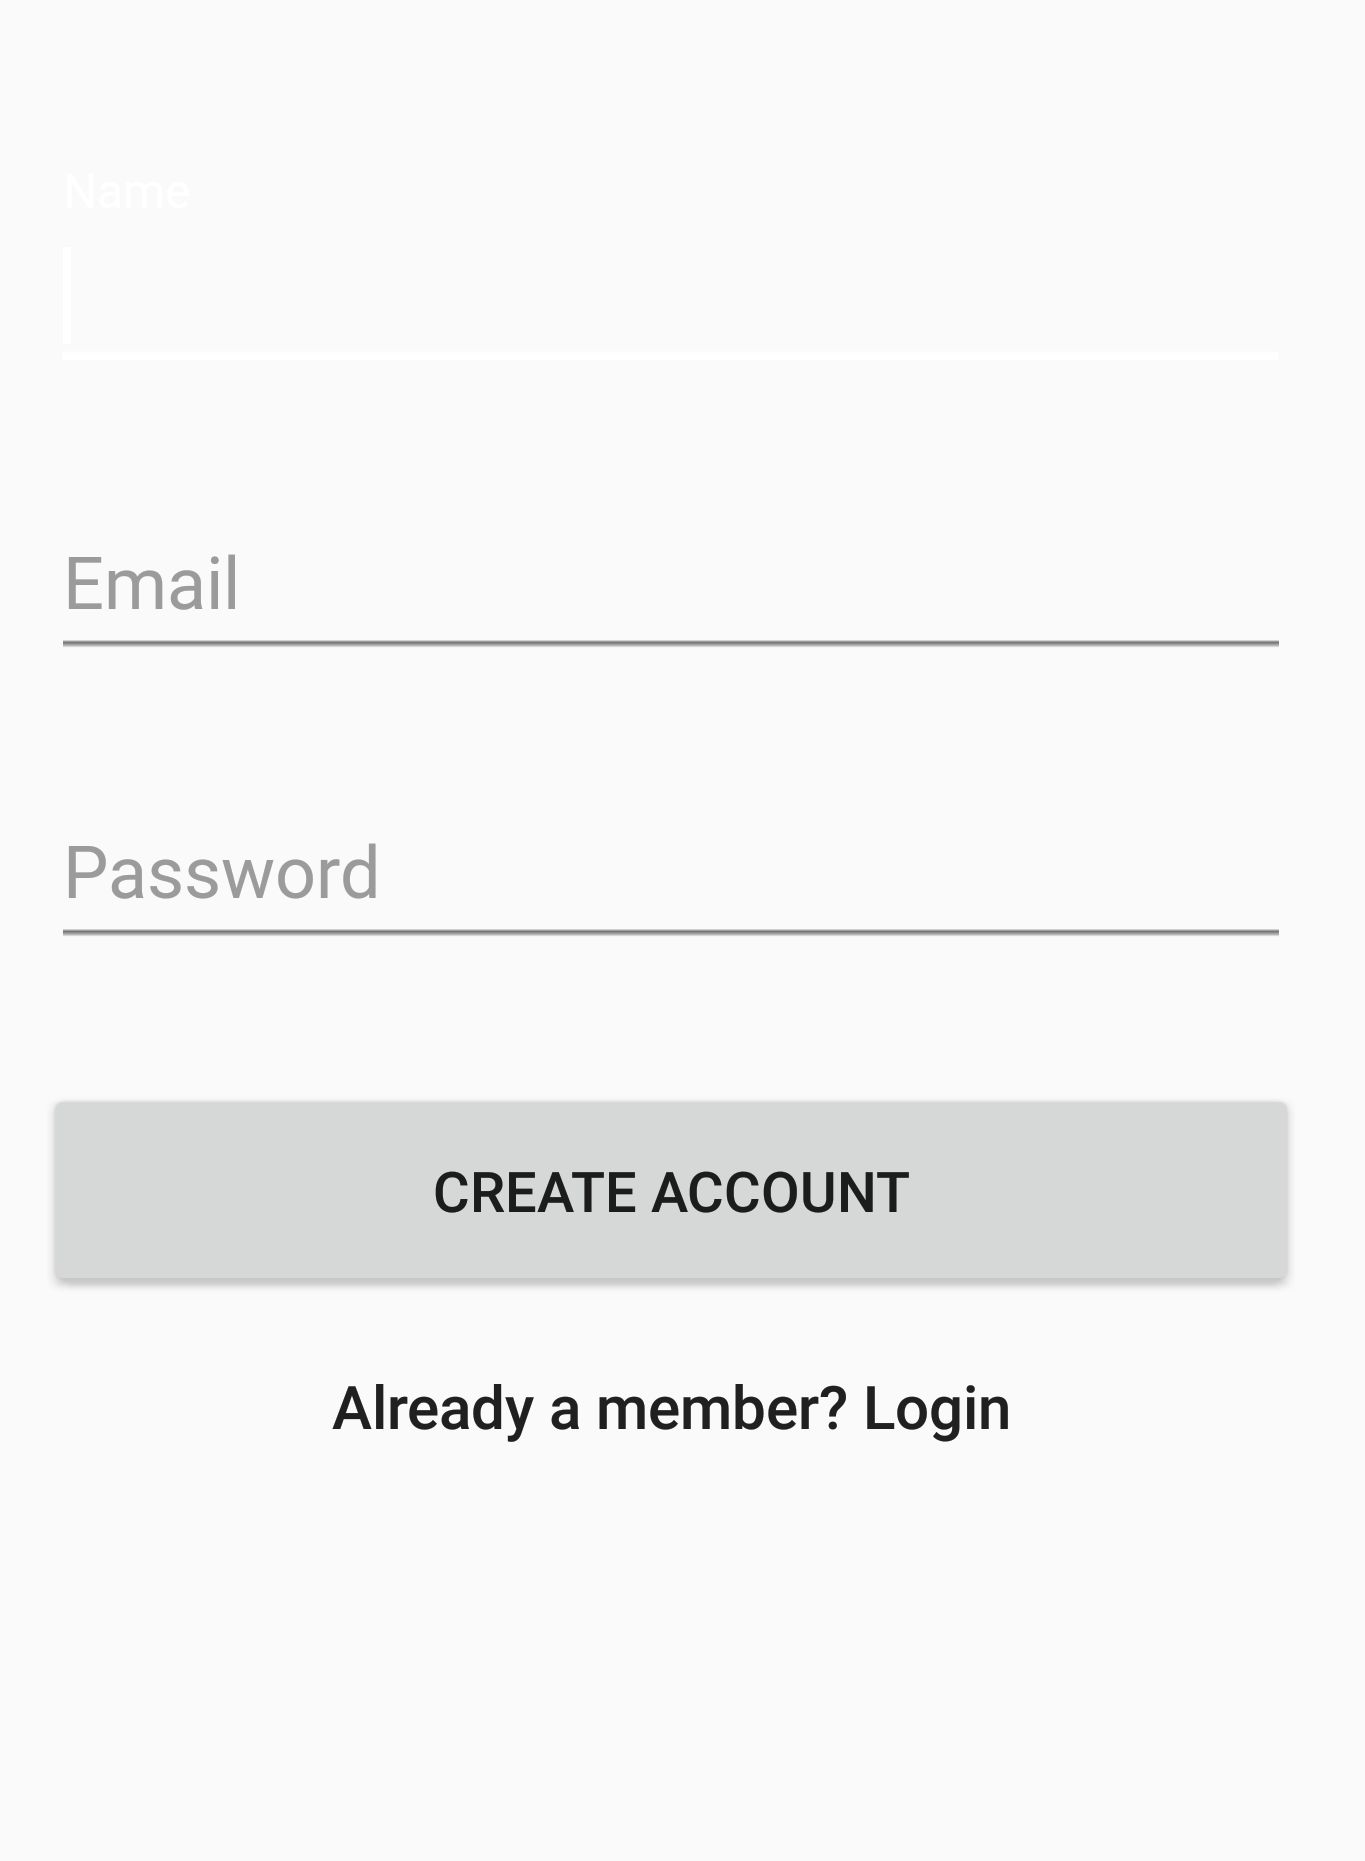
\includegraphics[width=0.40\textwidth]{register}
	\hfill
	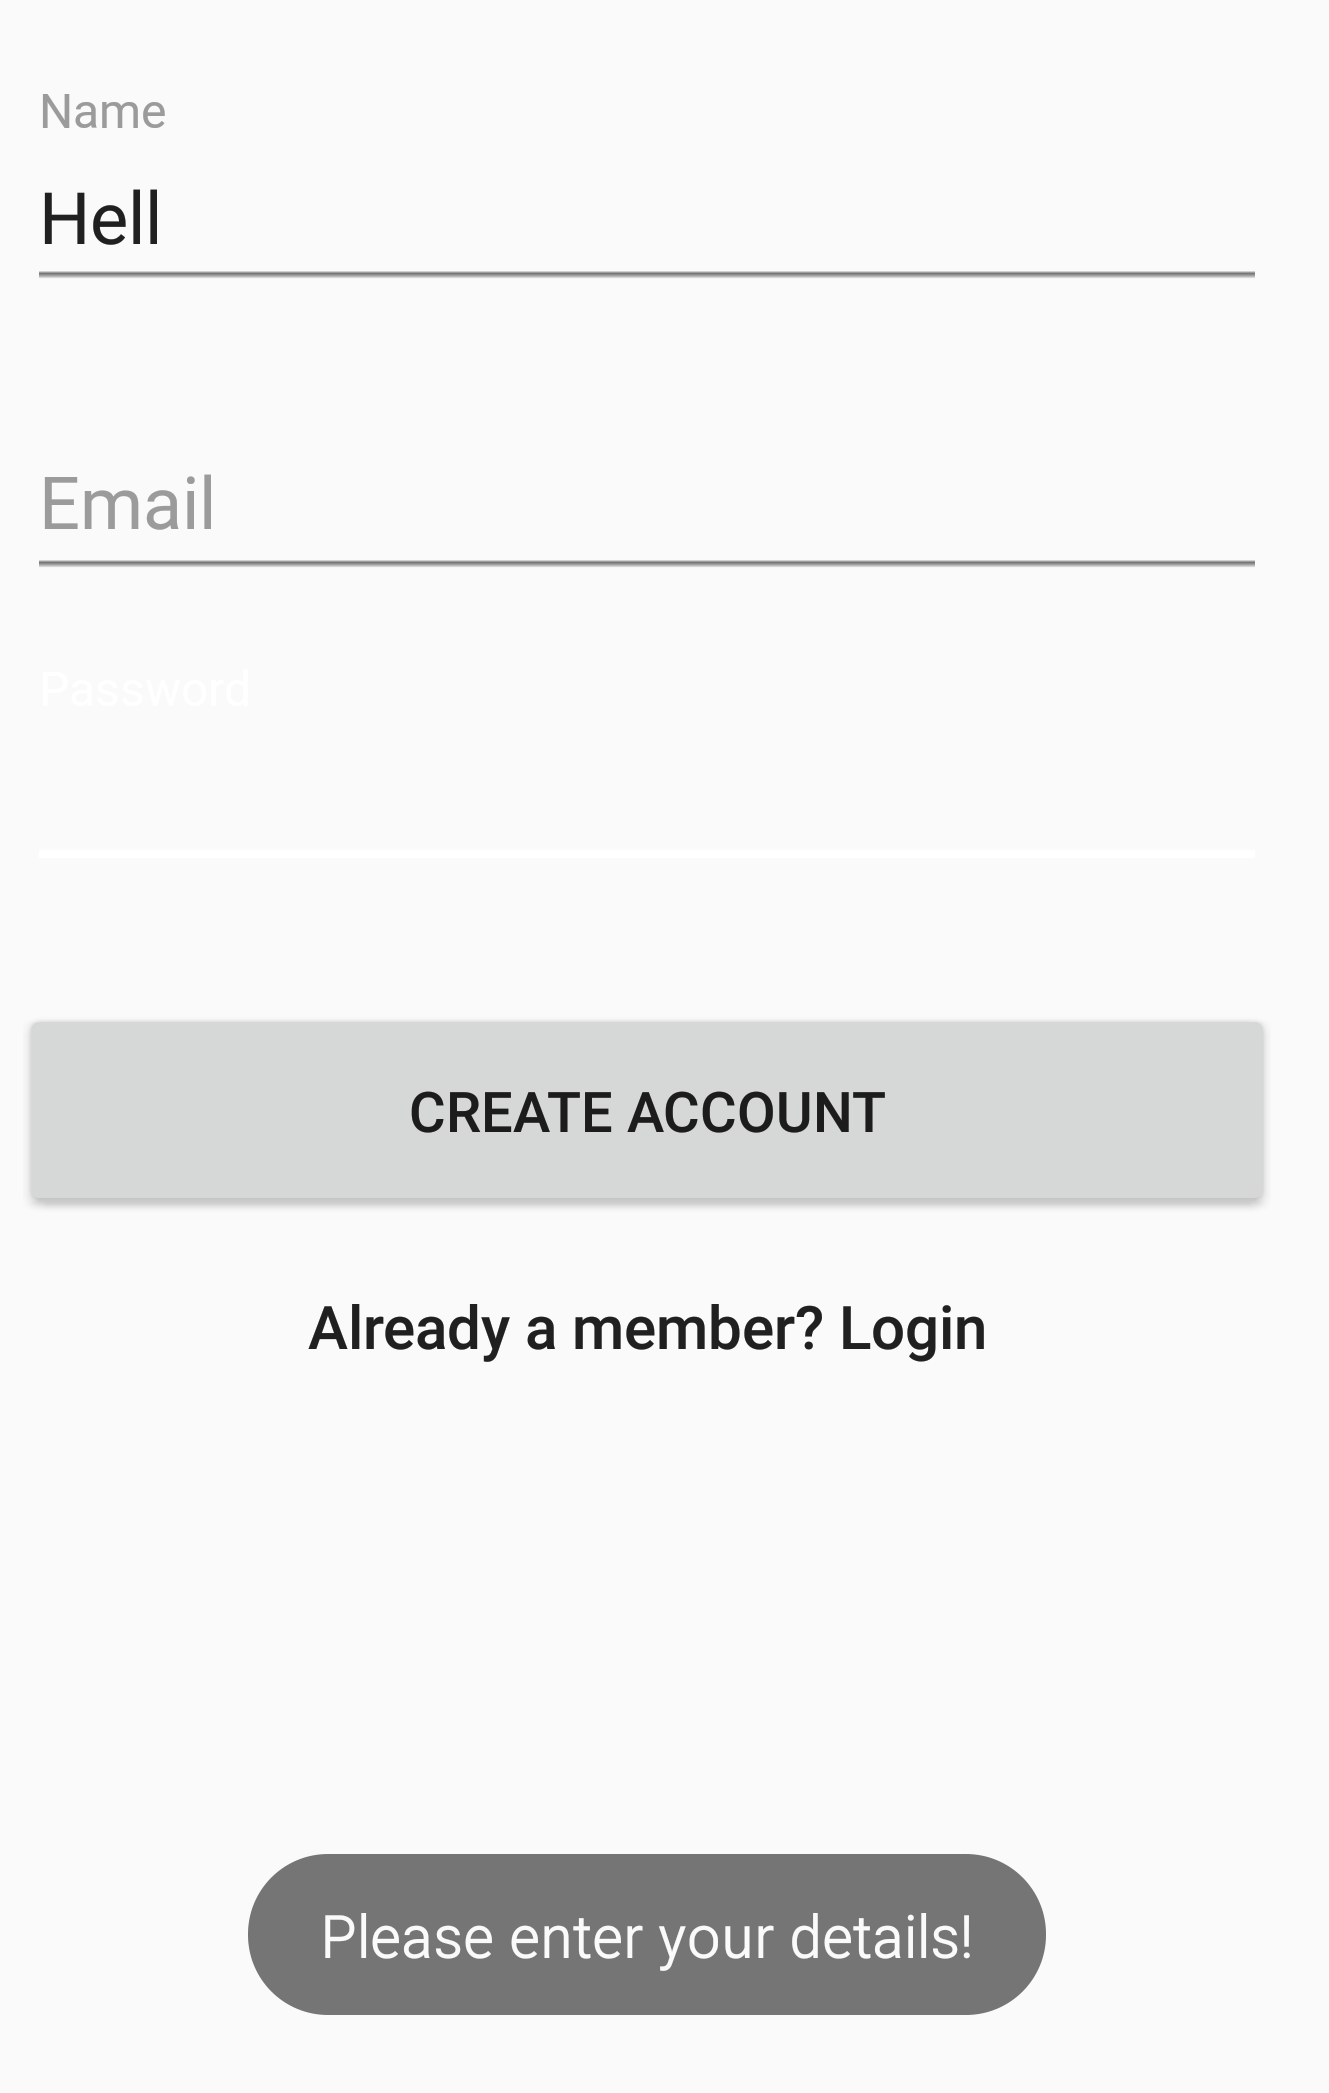
\includegraphics[width=0.40\textwidth]{register2}
	\caption{Register}
	\label{fig:register}
\end{figure}
So to register, users need to fill out all 3 rows: Name, Email and Password. If an email has already been registered or that not all fields have been filled a small message will show up like second image.\par
If user has already registered, clicking on \textbf{Already a member? Login} will redirect user to Login page as shown in figure \ref{fig:login}.\par
{\large 2. Login}\par
If user registered with the same email, the application will show a different message instead in the same style.\par
\begin{figure}[H]
	\centering
	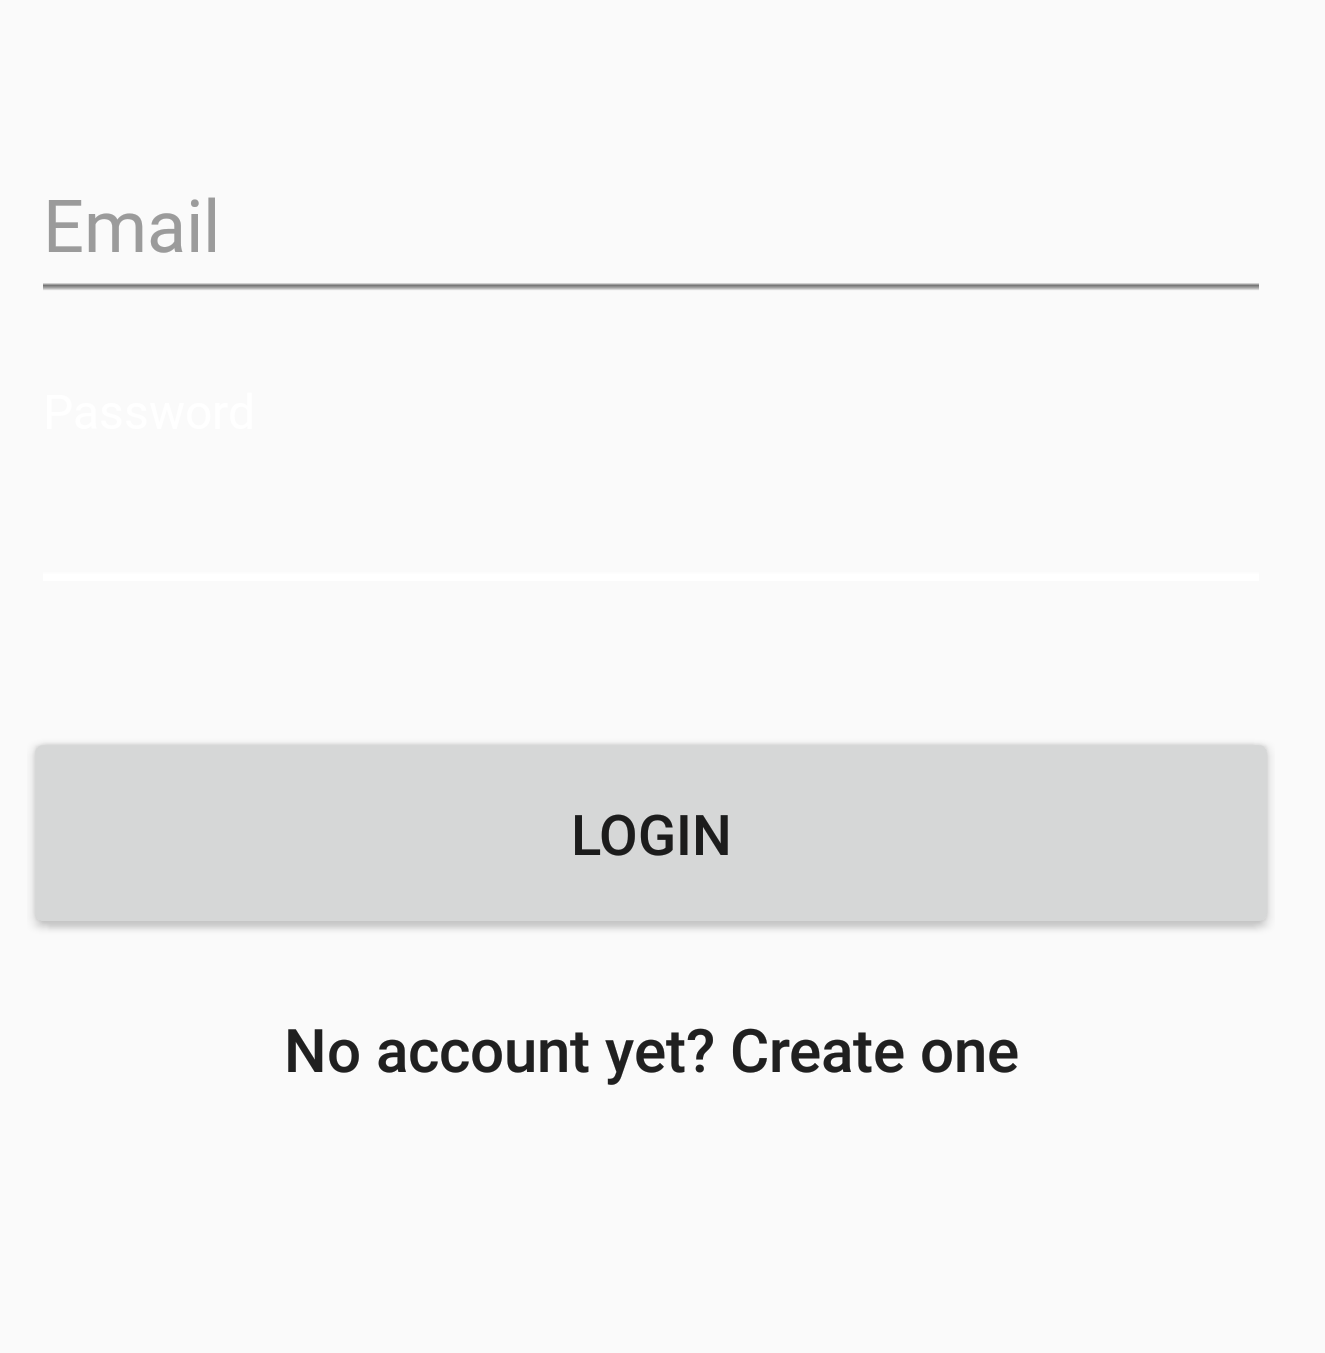
\includegraphics[width=0.40\textwidth]{login}
	\caption{Login}
	\label{fig:login}
\end{figure}
Login page, clicking on \textbf{No account yet? Create one} will redirect the user to register page.\par
{\large 3. Main Page}\par
\begin{figure}[H]
	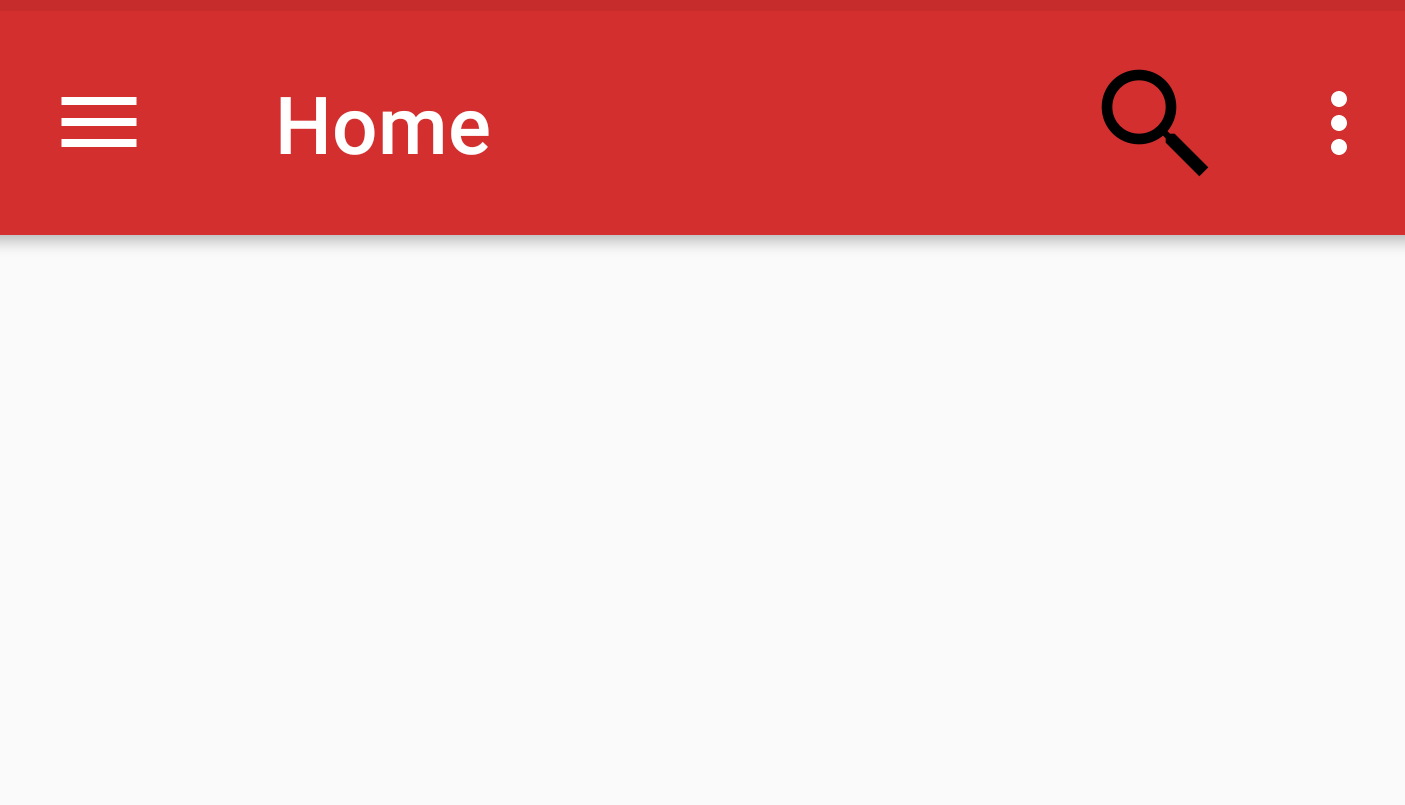
\includegraphics[width=0.40\textwidth]{main}
	\hfill
	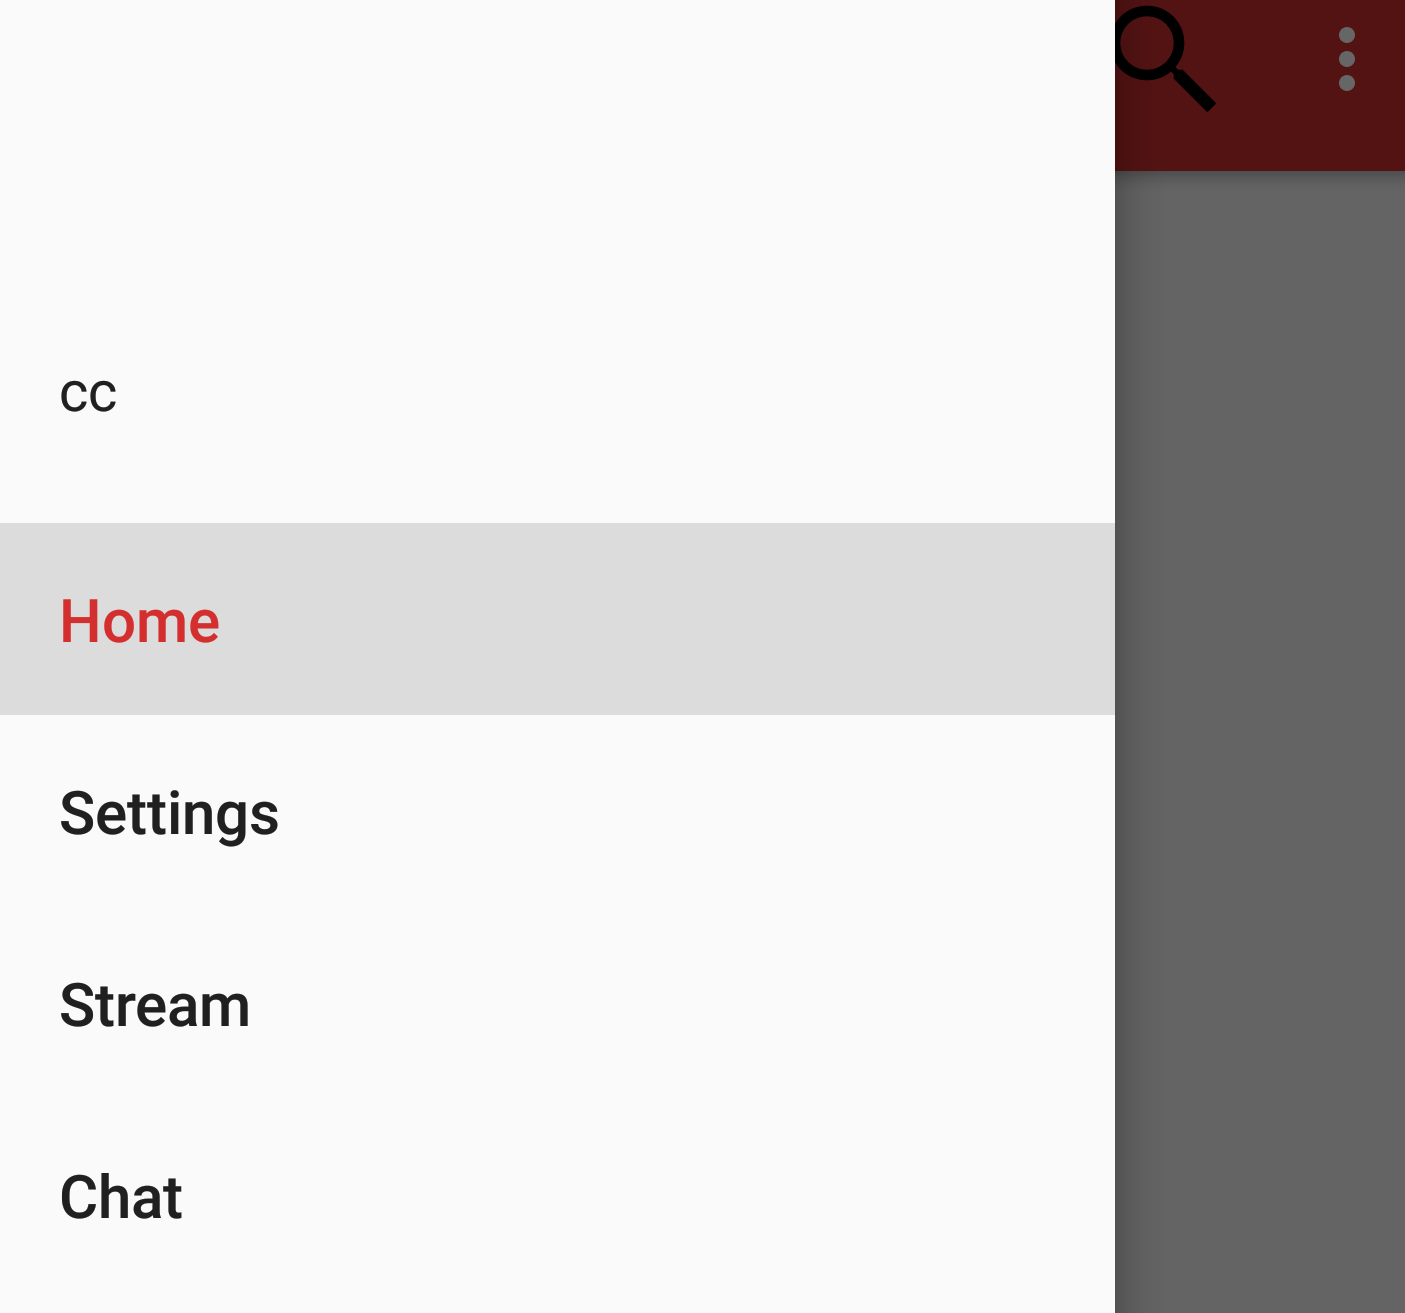
\includegraphics[width=0.40\textwidth]{main2}
	\caption{Main}
	\label{fig:main}
\end{figure}
Above image shows the first thing user will see after logging in, click on magnifying glass symbol to search for commentators by name. Next, the three dots shows two options: \textit{Log out} and \textit{Stream}, click on \textit{Stream} to listen to ongoing live stream.\par
Swiping left or clicking on the symbol next to \textbf{Home} will show the above window, user's name is shown on the top, go to \textbf{Settings} to register to be a commentator, \textbf{Stream} to begin broadcasting and \textbf{Chat} to enter the live chat room.\par
{\large 4. Stream Player}\par
\begin{figure}[H]
	\centering
	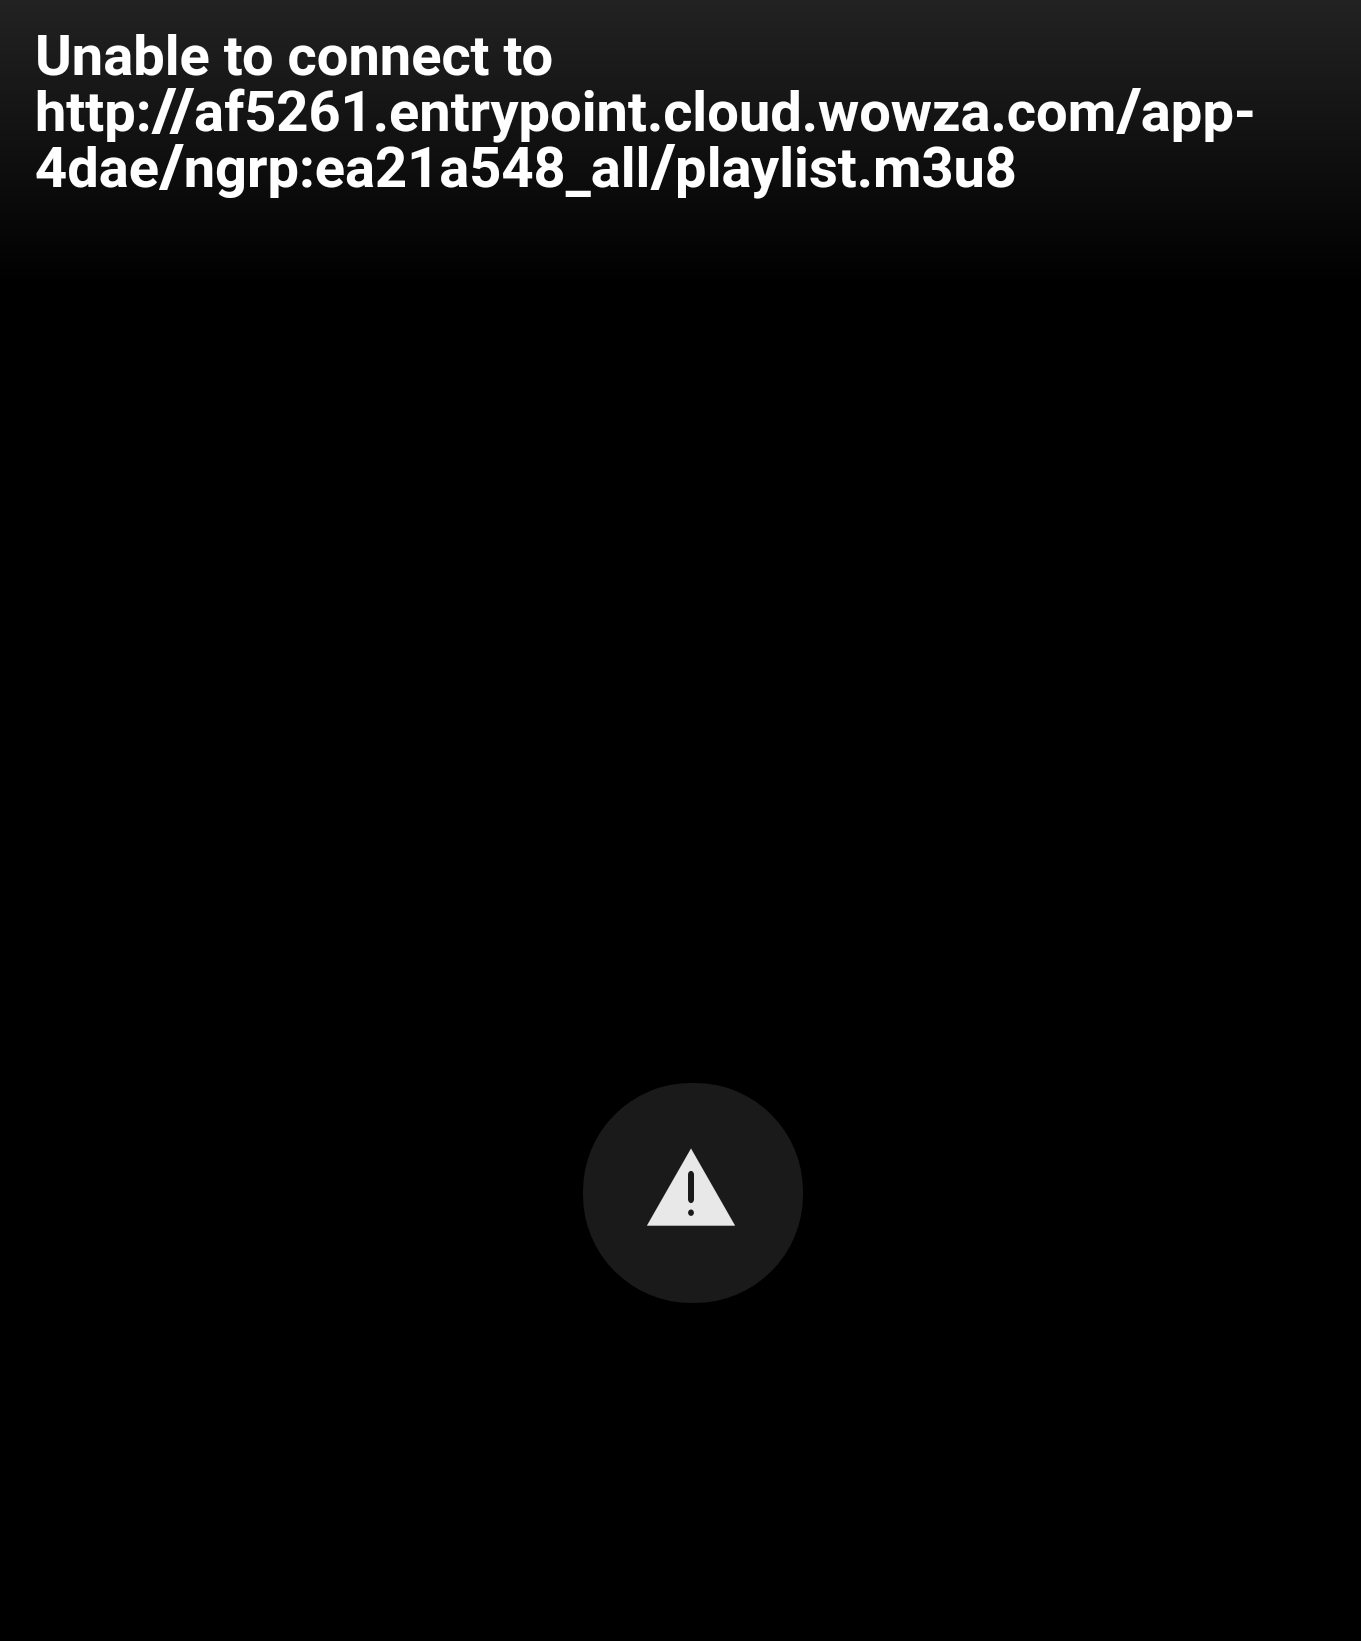
\includegraphics[width=0.40\textwidth]{player}
	\caption{Stream Player}
	\label{fig:player}
\end{figure}
This is the stream player view, normally if there's no current stream going on, the player will display the error message as above.\par
{\large 5. Settings}\par
\begin{figure}[H]
	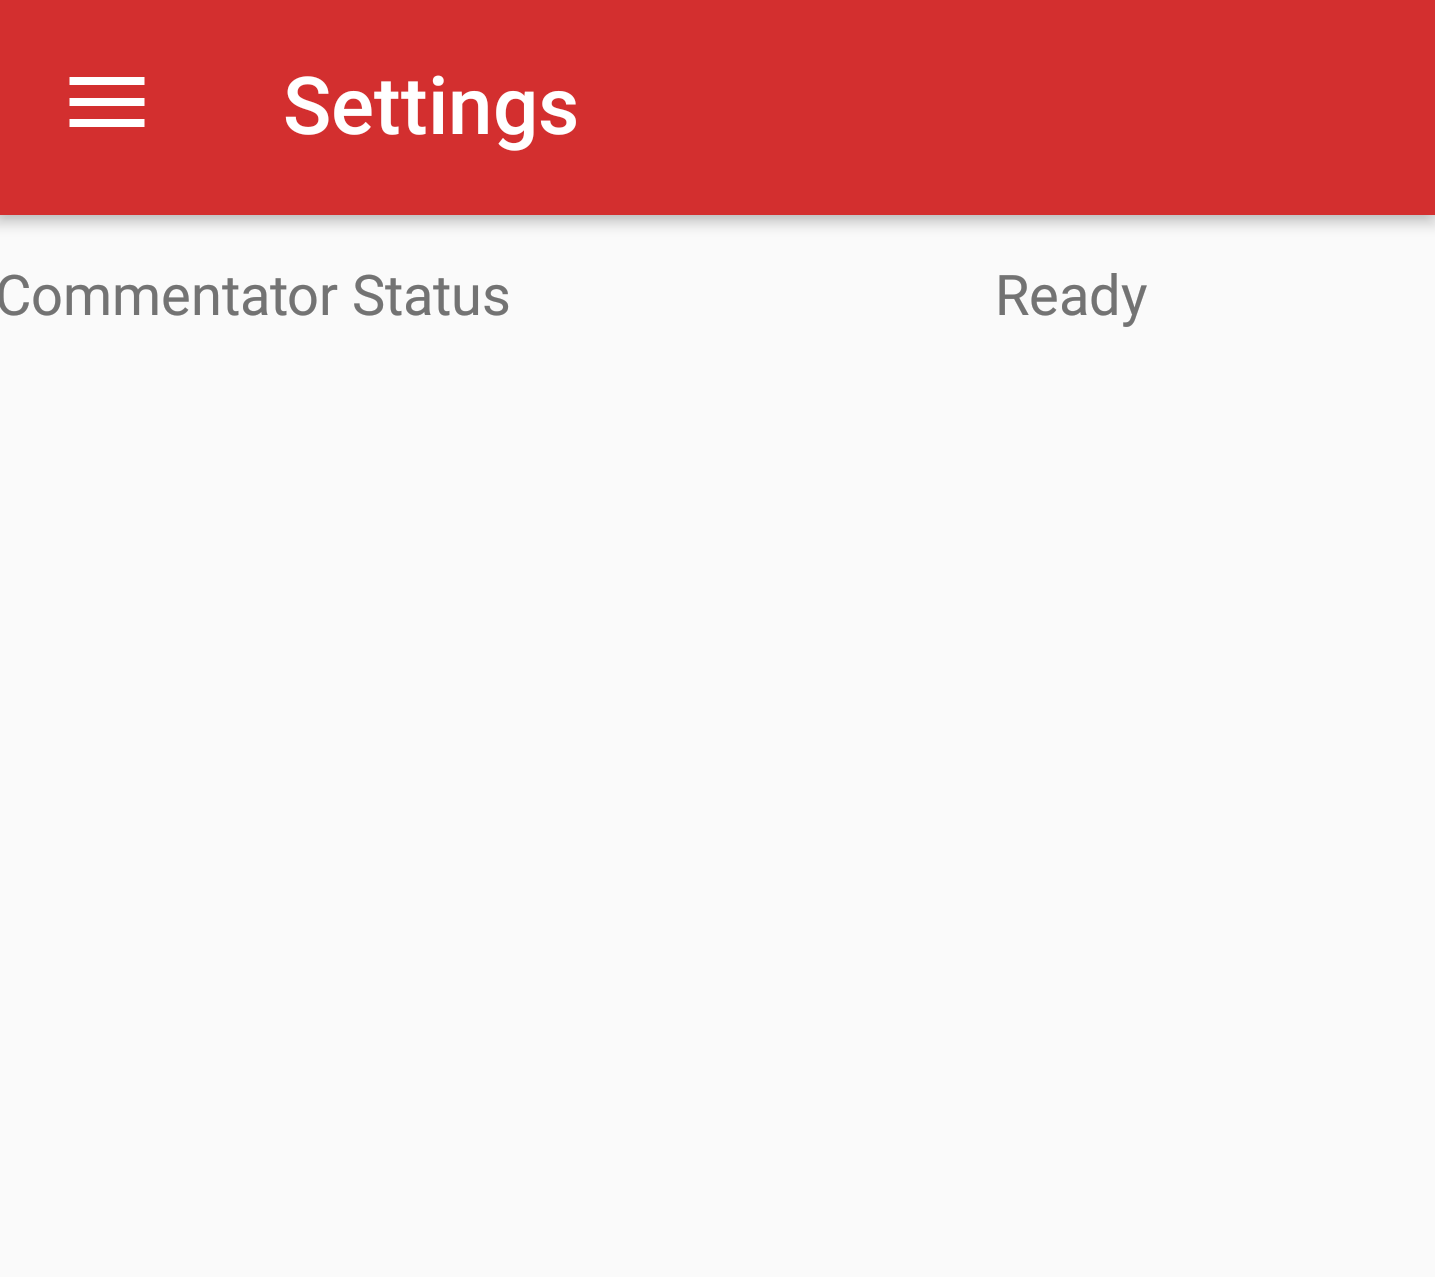
\includegraphics[width=0.40\textwidth]{settings}
	\hfill
	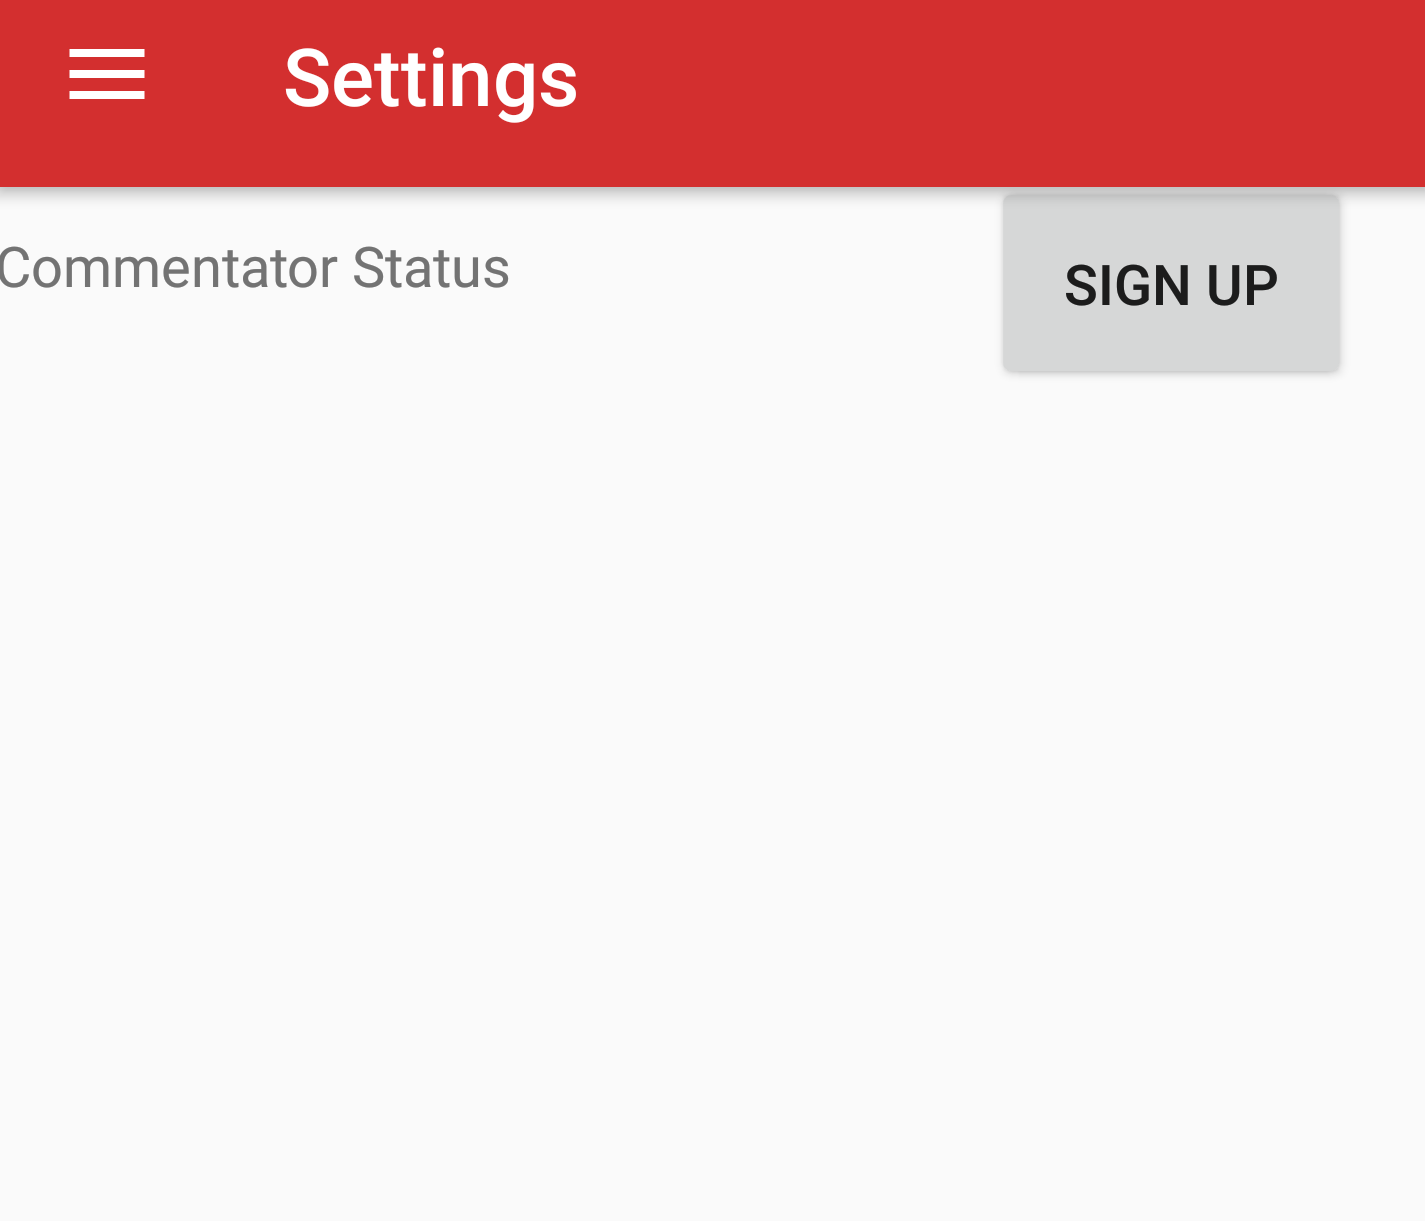
\includegraphics[width=0.40\textwidth]{settings2}
	\caption{Settings}
	\label{fig:settings}
\end{figure}
The above images demonstrate the difference a commentator and a normal user will see, upon clicking on \textbf{SIGN UP} button, the application will redirect user to figure \ref{fig:signup}
\begin{figure}[H]
	\centering
	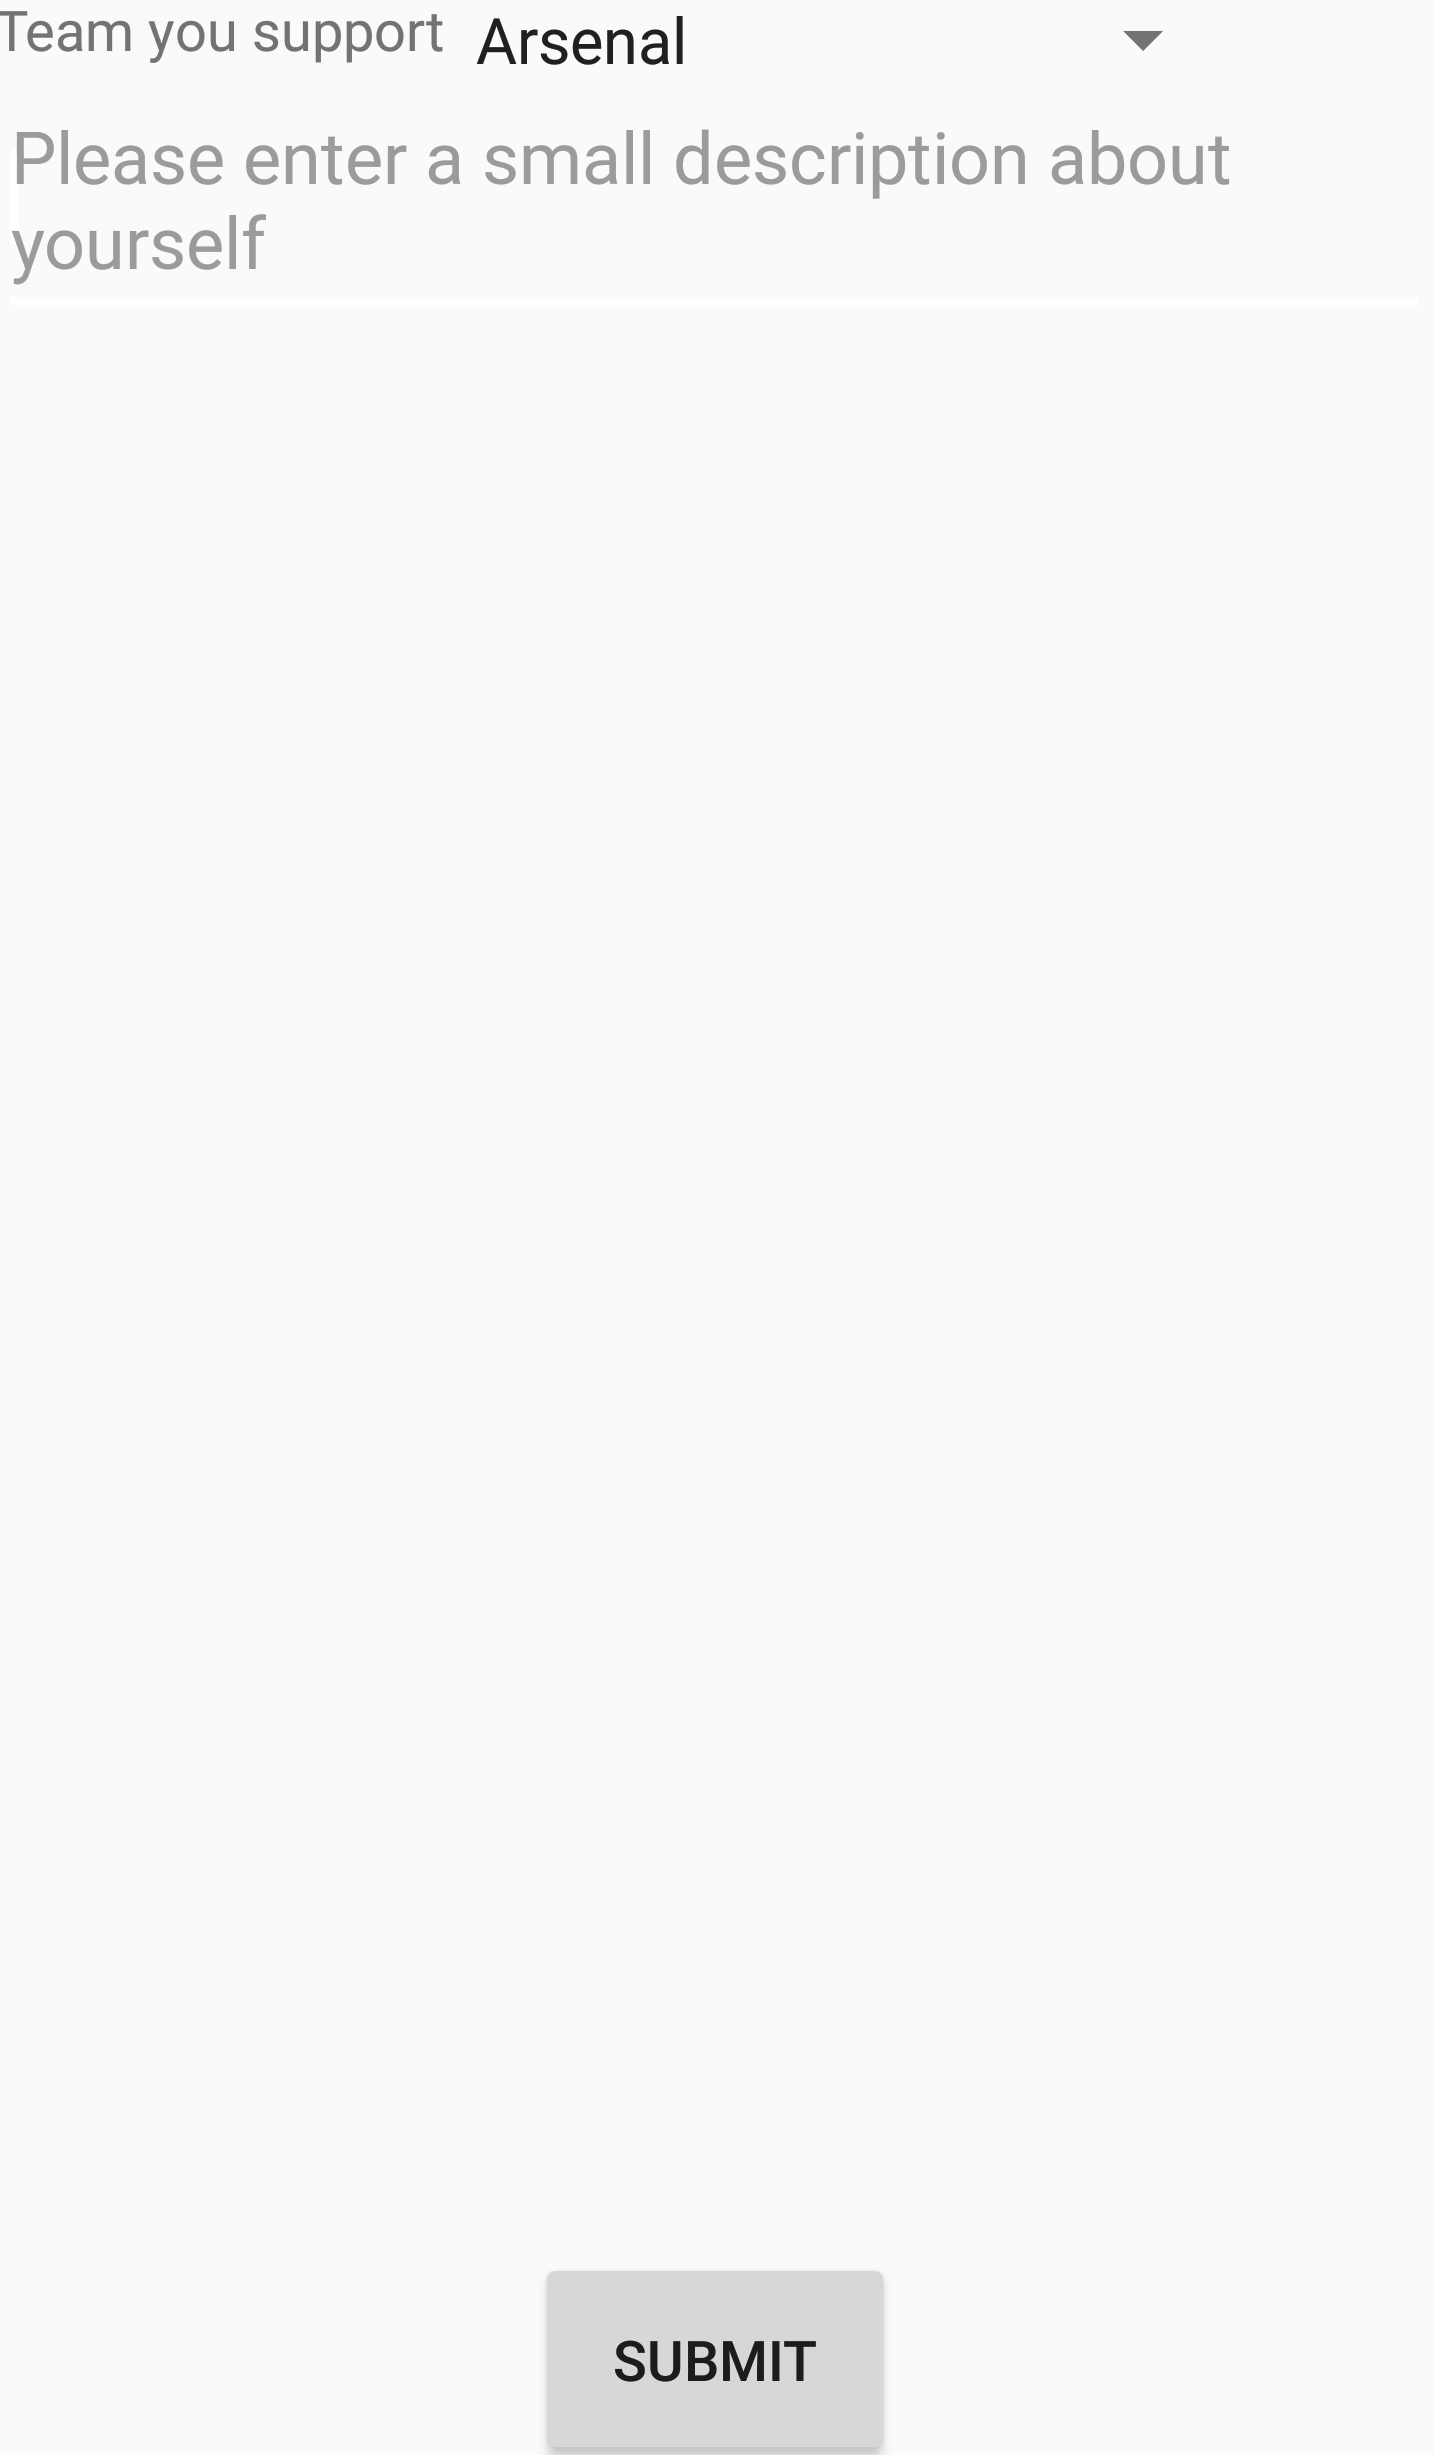
\includegraphics[width=0.40\textwidth]{signup}
	\caption{Commentator Sign Up Form}
	\label{fig:signup}
\end{figure}
Once the form has been submitted, application will redirect user back to log in page.\par
{\large 6. Streaming}\par
\begin{figure}[H]
	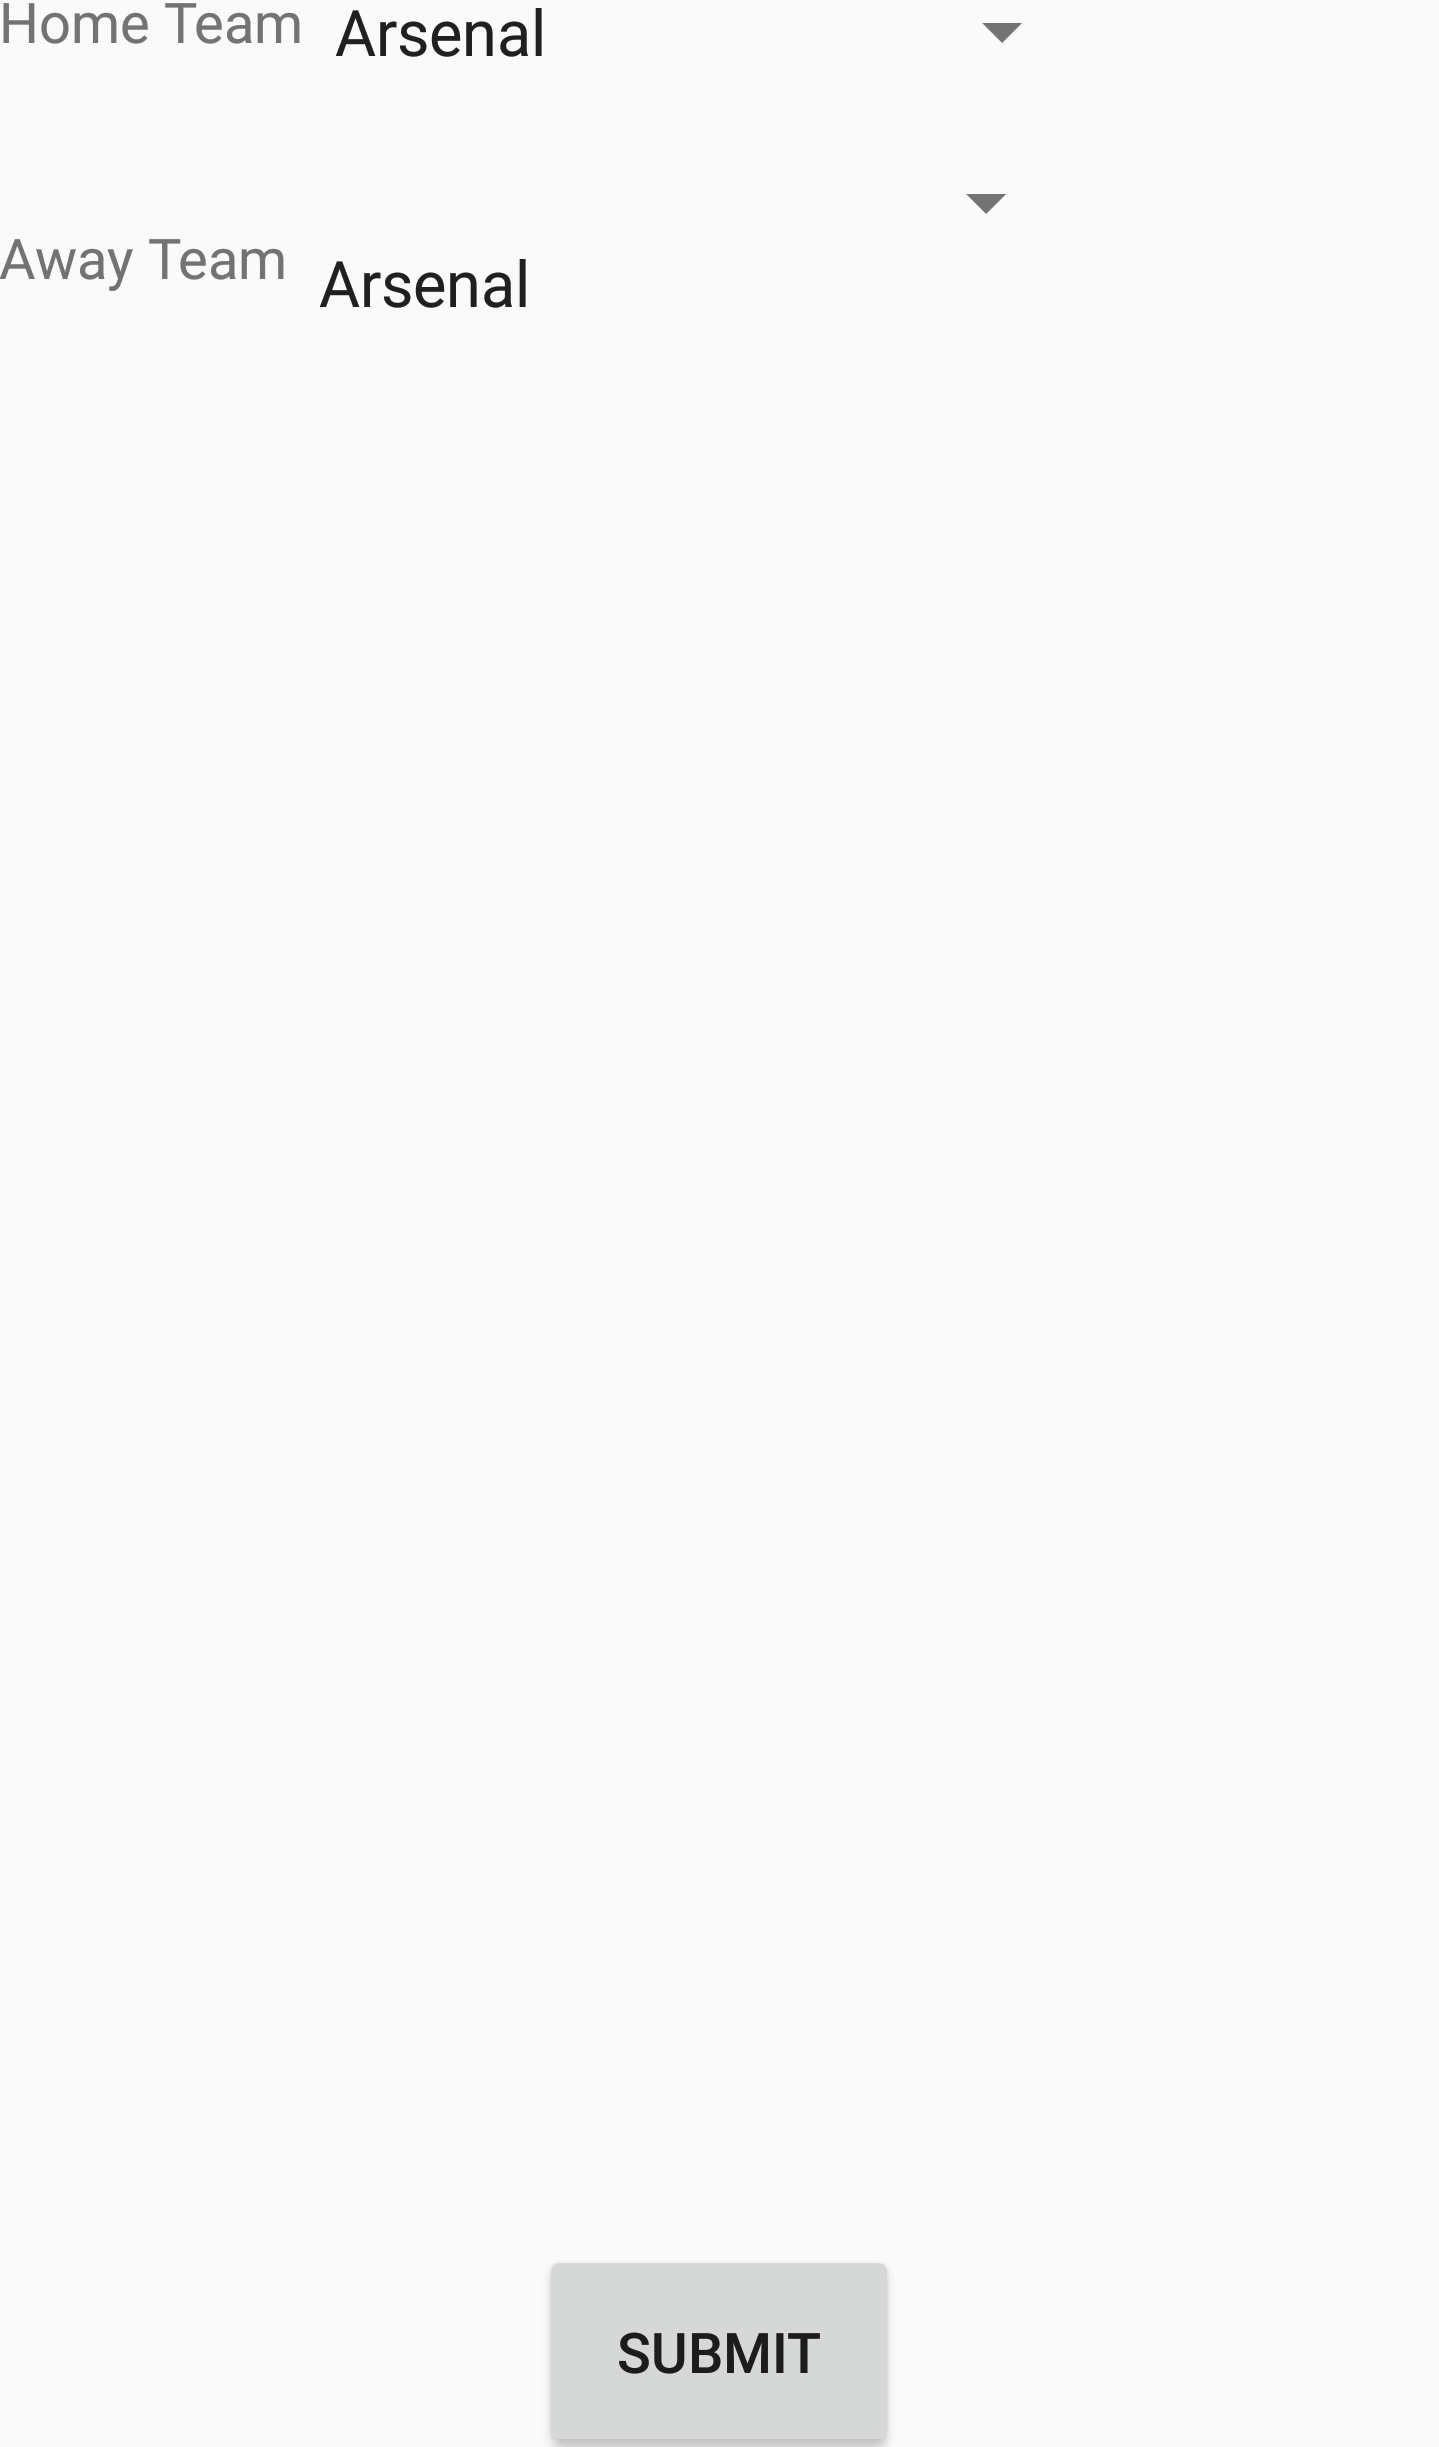
\includegraphics[width=0.40\textwidth]{matchmaking}
	\hfill
	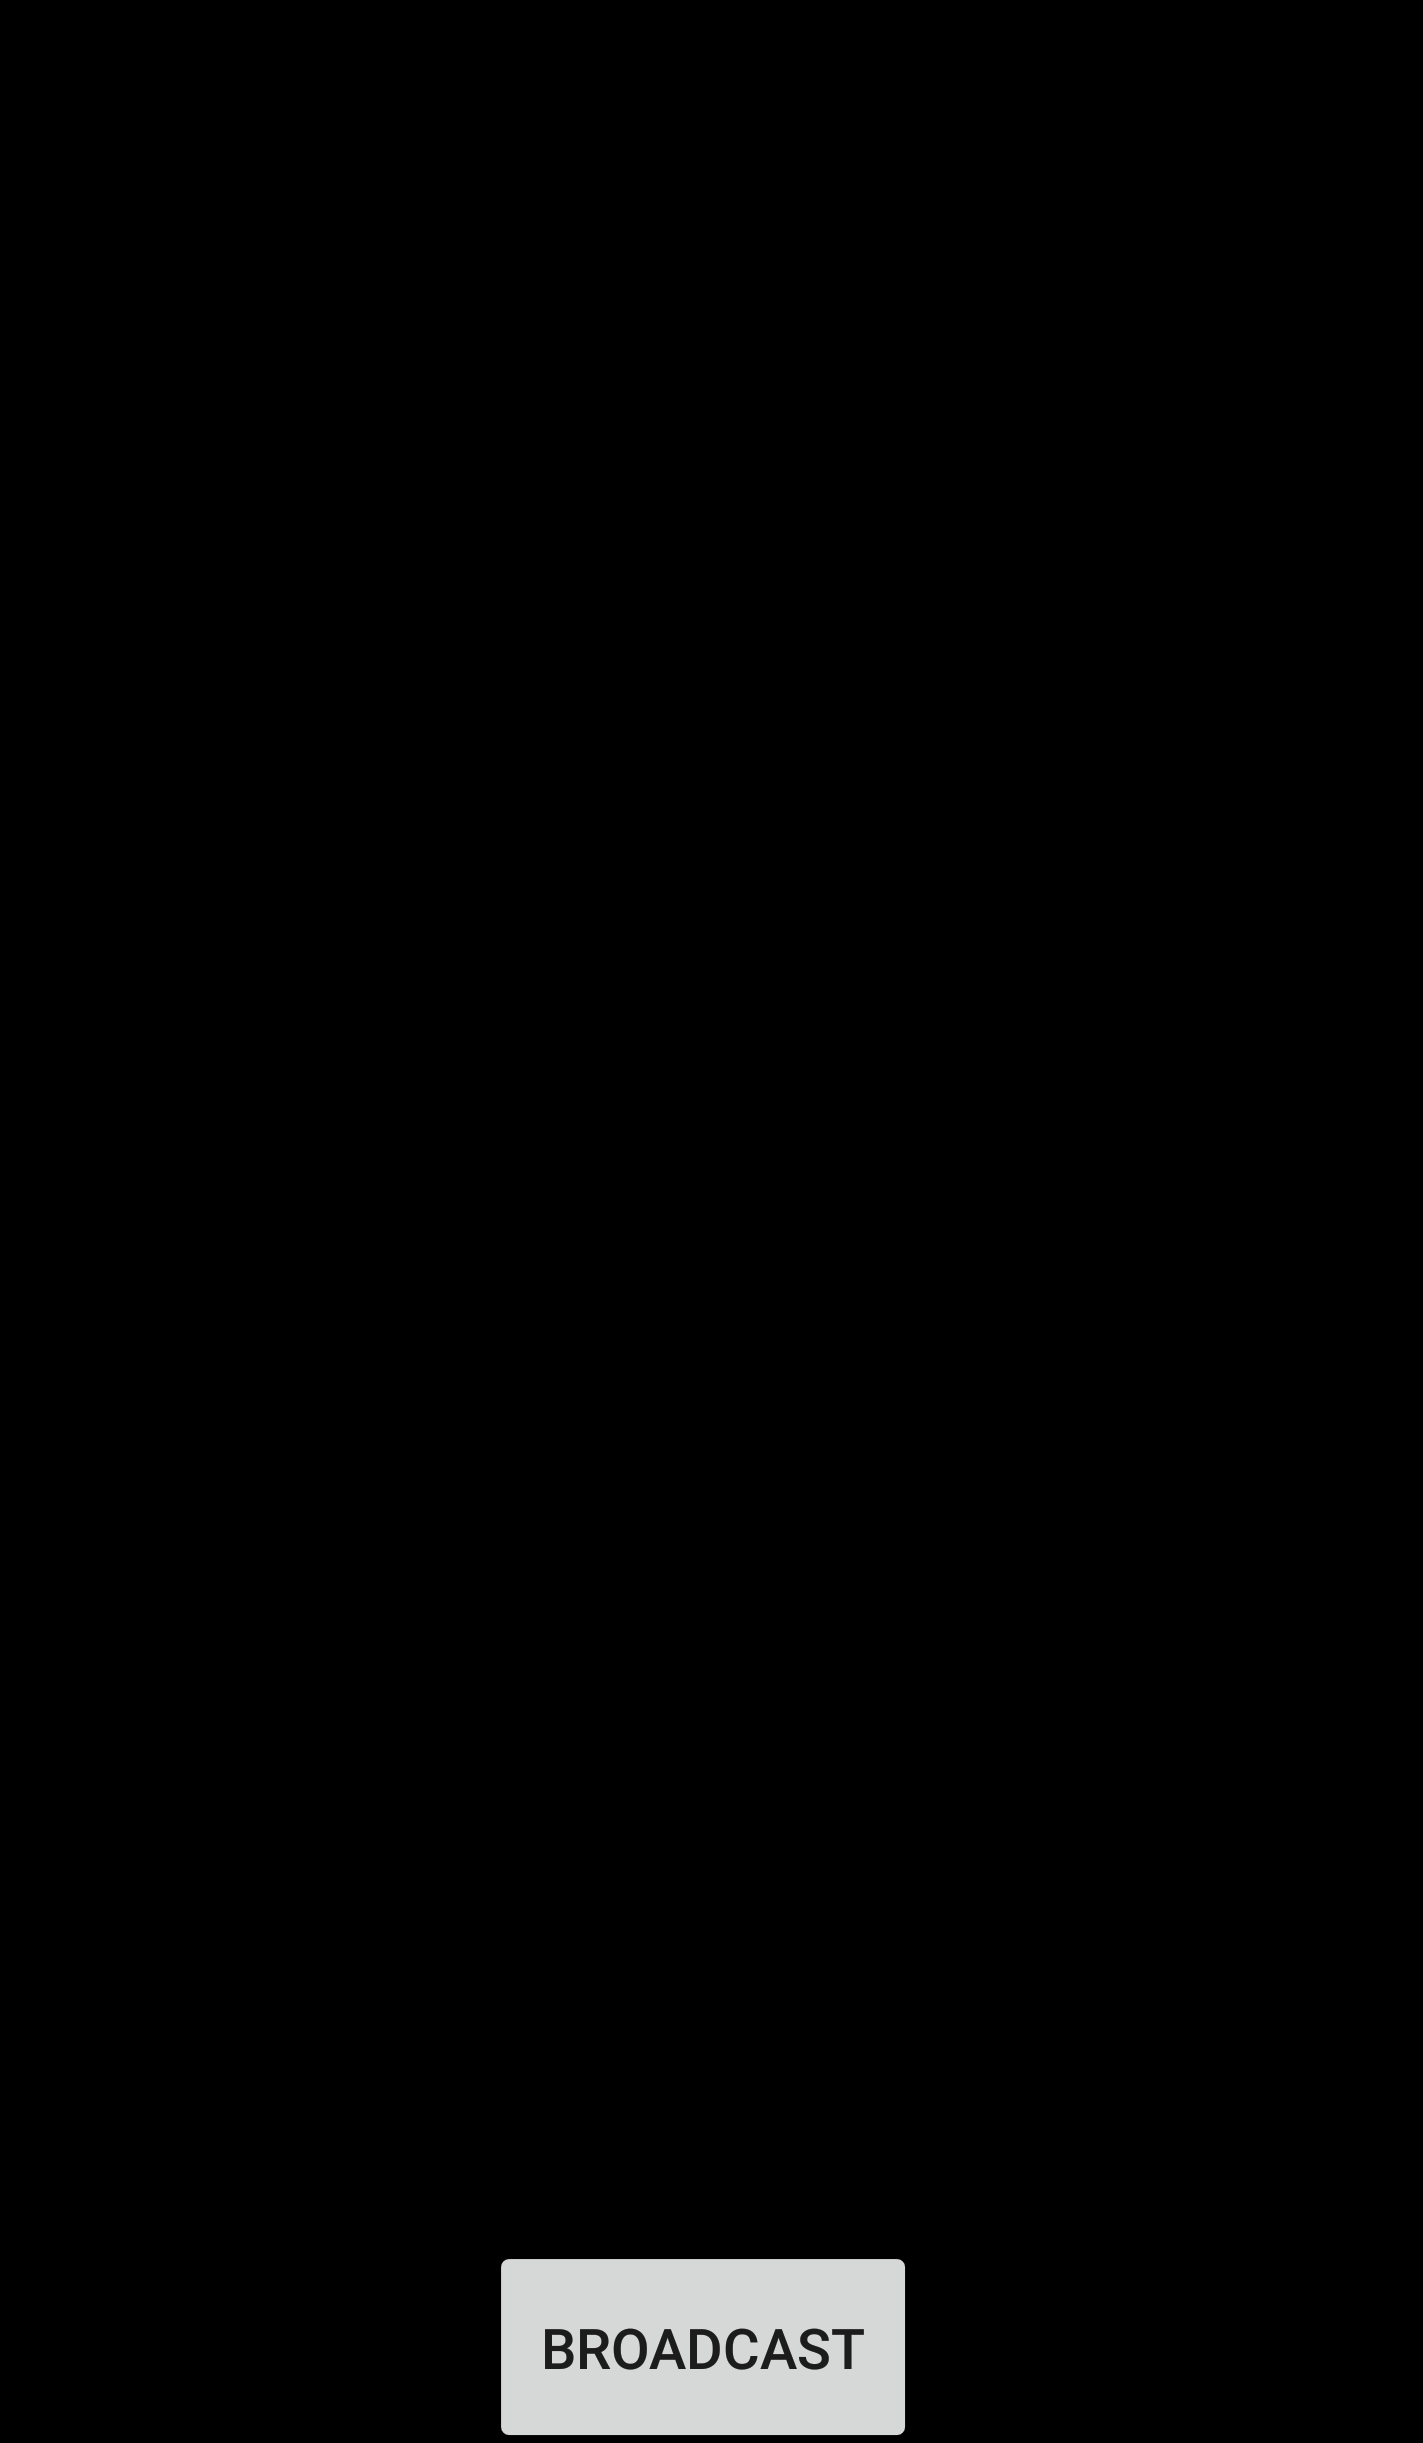
\includegraphics[width=0.40\textwidth]{broadcast}
	\caption{Broadcasting}
	\label{fig:broadcast}
\end{figure}
To broadcast, commentator will first have to fill out the form, in this activity there are few limitations: \textit{Home Team} and \textit{Away Team} can't be the same, GPS must be turned on and commentator has to be within 200 metres of \textit{Home Team}'s stadium. After that, commentator will be redirected to the next activity as shown in figure \ref{fig:broadcast} (The image is taken on Note 4 device, normally it will show a camera view instead). Presssing \textbf{BROADCAST} button will connect the to Wowza Streaming Cloud, the application will display at the bottom of page if it encountered any connection error.\par
{\large 7. Chat}\par
\begin{figure}[H]
	\centering
	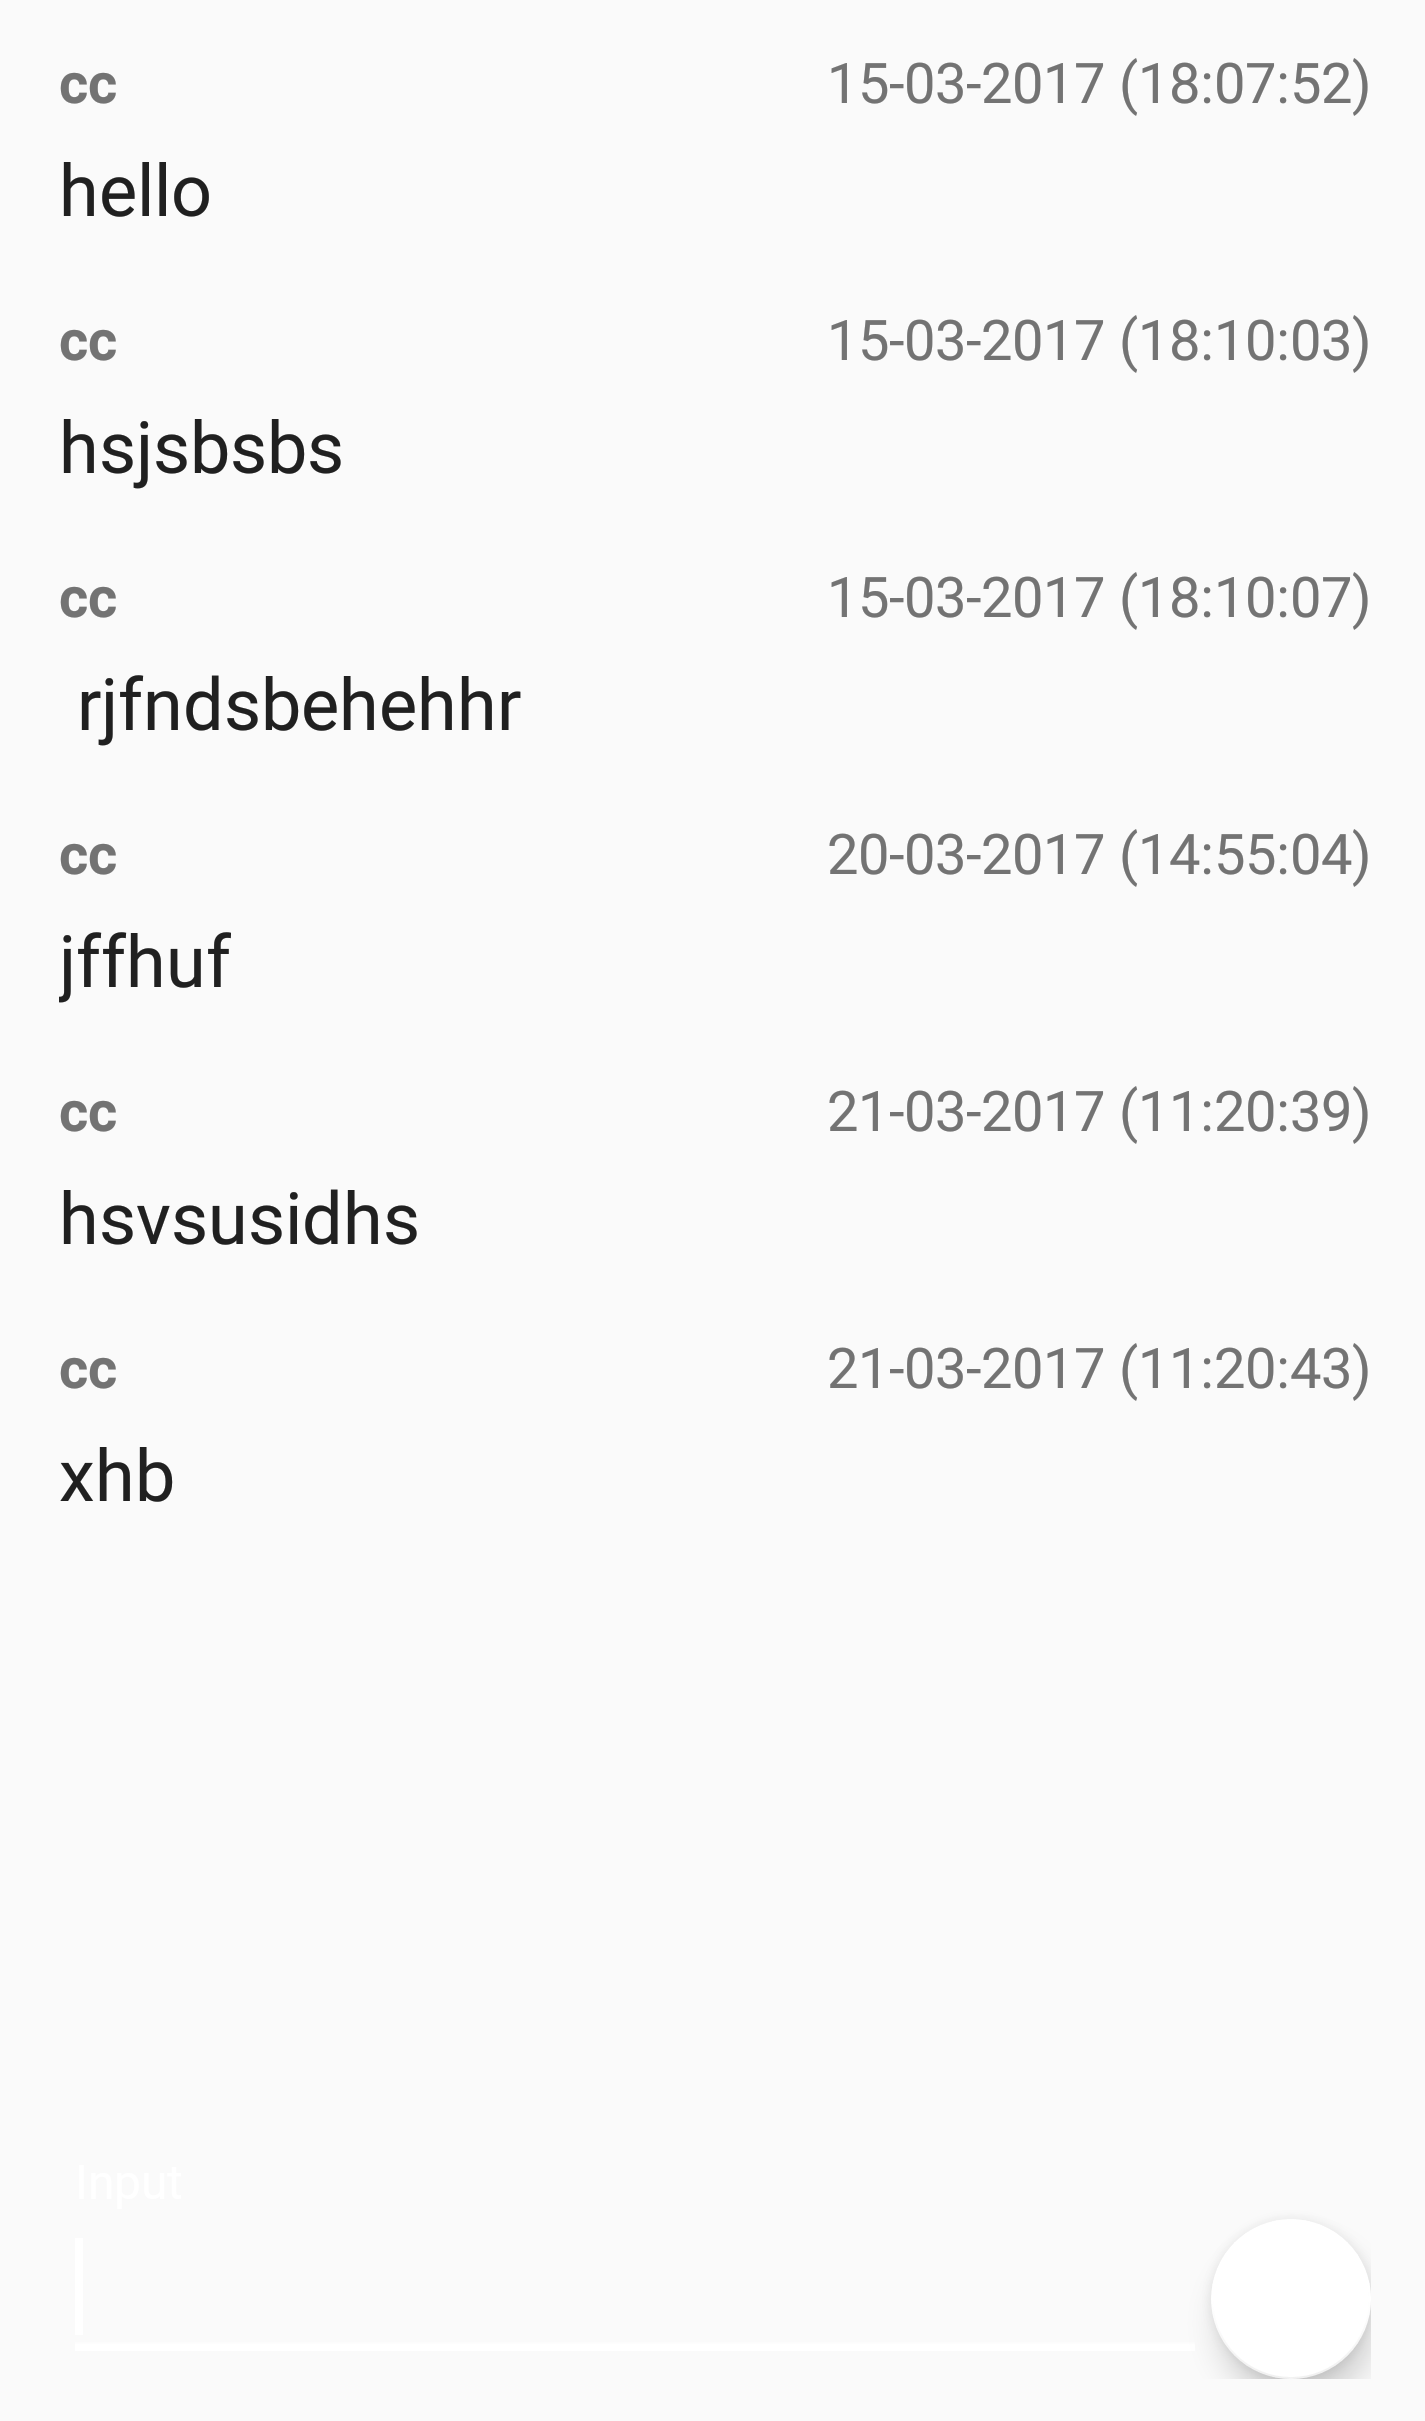
\includegraphics[width=0.40\textwidth]{chat}
	\caption{Live Chat Room}
	\label{fig:chat}
\end{figure}
The chat room model is pretty simple, it shows only name of the sender, message content and time the message was sent. The big white circle is used to send message.\par
{\Large \textbf{Appendix F}}\par
{\huge Project Plan and Interim Report}\par
{\large 1. Project Plan}\par
\end{flushleft}
\newpage
\begin{center}
{\Huge Live Audio Commentary\\[5cm]}

{\Large Sam Mai

BSc Computer Science

Submission Date: 16\textsuperscript{th} November 2016

Supervisor: Harry Strange}
\end{center}
\newpage
\begin{flushleft}
{\Large \underline{Aims:}}\par
To develop a socialising Android application where football fans can interact with each other. The application will allow users to listen to live audio commentaries hosted by other users more specifically commentators. Users can share their own thoughts and insights by registering to become a commentator and record their own commentaries.\par
{\Large \underline{Objectives:}}
\begin{itemize}
	\item To allow users to follow football games from others’ points of view through live commentaries.
	\item To allow users to share their thoughts and insights about football games through live commentaries.
	\item To allow users to express their views on quality of commentaries from different commentators.
	\item To offer practices to users who are interested in doing audio commentaries.
	\item To allow users to interact with each other in a friendly manner.
\end{itemize}
{\Large \underline{Deliverables:}}
\begin{itemize}
	\item A design specification for the Android application.
	\item A fully documented and functional Android application.
	\item A strategy for testing and evaluating the Android application.
\end{itemize}
{\Large \underline{Work Plan:}}
\begin{itemize}
	\item 28/10/16 – 14/11/16: Literature Search and Review
	\begin{itemize}
		\item Defining Aims and Objectives 
		\item Cloud Platform Research 
	\end{itemize}
	\item 01/11/16 – 14/11/16: Project Plan
	\item 01/11/16 – 22/11/16: Analysis and Modelling
	\begin{itemize}
		\item MoSCoW Requirements 
		\item Use Cases 
		\item System Diagrams
	\end{itemize}
	\item 22/11/16 – 12/12/16: System Design and Prototypes
	\begin{itemize}
		\item UI design 
		\item Initial Prototype 
		\item System Architecture
	\end{itemize} 
	\item 12/12/16 – 07/02/17: System Implementation
	\begin{itemize}
		\item Configuring Cloud Service
		\item Coding
	\end{itemize}
	\item 10/01/17 – 25/01/17: Interim Report
	\item 07/02/17 – 07/03/17: Testing and Evaluation
	\begin{itemize}
		\item Code Refactoring
		\item Functional Testing
	\end{itemize}
	\item 07/03/17 – 11/04/17: Final Report
\end{itemize}
{\large 2. Interim Report}
\end{flushleft}
\newpage
\begin{center}
{\Huge Live Audio Commentary\\[5cm]}

{\Large Sam Mai

BSc Computer Science

Submission Date: 16\textsuperscript{th} November 2016

Supervisor: Harry Strange}
\end{center}
\newpage
\begin{flushleft}
{\large \textbf{Progress made to date}}\par
I have completed 50\% of all the must requirements during the last term.\par
I have finalised the UI of the application and implementing the UI as I’m developing other features of the app. Currently the app has the login, register, main and search page. This equates to roughly 50\% of the whole UI of the application.\par
User authentication system is finished, users should now be able register and login at this stage. Database is hosted on 000webhost.com, where the application would make a REST call to the scripts on the website to interact with the database.\par
Search functionality is partially completed; users can search for commentators by name. In theory, users should also be able to search for commentaries in the same way.\par
I have also implemented the GPS functionality to check for users’ current locations.\par
{\large \textbf{Remaining work to be done before the final report deadline}}\par
Recently switched up the streaming cloud service from Azure Media Services to Wowza, streaming functionality should be completed soon enough in 1-2 weeks’ time.\par
Commentators’ profile is another requirement needs to be fulfilled. This is a relatively small task and should be finished in the upcoming week or at the latest in 2 weeks’ time.\par
Sorting of search results based on commentators’ ratings is another requirement needs implemented.\par
Also live chat is another requirement left to be done and will probably be the last thing on schedule to be finished.\par
{\Large \textbf{Appendix G}}\par
{\huge Code Listing}\\
{\large \textit{SearchableActivity.class}}
\end{flushleft}
\begin{landscape}
\begin{lstlisting}[language=Java, basicstyle=\tiny]
public class SearchableActivity extends ListActivity {

    private ProgressDialog pDialog;
    private final String API_BASE_URL = "http://audiocommentary.000webhostapp.com";

    @Override
    public void onCreate(Bundle savedInstanceState) {
        super.onCreate(savedInstanceState);
        setContentView(R.layout.container_list);

        // Progress dialog
        pDialog = new ProgressDialog(this);
        pDialog.setCancelable(false);

        handleIntent(getIntent());
    }

    @Override
    protected void onNewIntent(Intent intent) {
        setIntent(intent);
        handleIntent(intent);
    }

    private void handleIntent(Intent intent) {
        if (Intent.ACTION_SEARCH.equals(intent.getAction())) {
            String query = intent.getStringExtra(SearchManager.QUERY);
            doMySearch(query);
        }
    }

    private void doMySearch(String query) {
        pDialog.setMessage("Searching...");
        showDialog();

        final Database databaseService = ServiceGenerator.getClient(API_BASE_URL).create(Database.class);
        Call<ResponseBody> response = databaseService.user_search(query);
        response.enqueue(new Callback<ResponseBody>() {
            @Override
            public void onResponse(Call<ResponseBody> call, Response<ResponseBody> response) {
                hideDialog();

                try {
                    if(response.isSuccessful()) {
                        String result = response.body().string();
                        result = result.substring(result.indexOf('{'));
                        JSONObject jObj = new JSONObject(result);
                        boolean error = jObj.getBoolean("error");
                        // Check for error node in json
                        if (!error) {
                            final JSONArray names = jObj.getJSONArray("users");
                            String values[] = new String[names.length()];
                            for(int i = 0; i < names.length(); i++) {
                                values[i] = names.getJSONObject(i).getString("name");
                                Log.d("VS",values[i]);
                            }
                            ArrayAdapter<String> arrayAdapter = new ArrayAdapter<String>(
                                    getApplicationContext(),
                                    R.layout.container_list_item_view,
                                    R.id.list_item,
                                    values
                            );
                            ListView lv = (ListView) findViewById(android.R.id.list);
                            lv.setAdapter(arrayAdapter);
                            lv.setEnabled(true);
                            lv.setOnItemClickListener(new AdapterView.OnItemClickListener() {
                                @Override
                                public void onItemClick(AdapterView<?> parent, View view, int position, long id) {
                                    try {
                                        JSONObject mInfo = names.getJSONObject(position);
                                        Log.d("SearchableActivity",mInfo.toString());
                                        final String name = mInfo.getString("name");
                                        getCommentatorProfile(name, mInfo.getString("user_id"),databaseService);
                                    } catch(Exception e) {
                                        e.printStackTrace();
                                    }
                                }
                            });


                        } else {
                            // Wrong request or users not found
                            String errorMsg = jObj.getString("error_msg");
                            Toast.makeText(getApplicationContext(),
                                    errorMsg, Toast.LENGTH_LONG).show();

                            //TextView lv = (TextView) findViewById(android.R.id.empty);

                        }
                    }
                    else {
                        // Error in request. Get the error message
                        String errorMsg = response.message();
                        Toast.makeText(getApplicationContext(),
                                errorMsg, Toast.LENGTH_LONG).show();
                    }

                } catch (Exception e) {
                    e.printStackTrace();
                }
            }

            @Override
            public void onFailure(Call<ResponseBody> call, Throwable t) {
                hideDialog();
            }
        });
    }

    private void getCommentatorProfile(final String name, final String userID, Database databaseService) {
        pDialog.setMessage("Loading...");
        showDialog();

        Call<ResponseBody> response = databaseService.get_commentator(userID);
        response.enqueue(new Callback<ResponseBody>() {
            @Override
            public void onResponse(Call<ResponseBody> call, Response<ResponseBody> response) {
                hideDialog();

                try {
                    if(response.isSuccessful()) {
                        JSONObject jObj = new JSONObject(response.body().string());
                        boolean error = jObj.getBoolean("error");
                        if(!error) {
                            JSONObject commentator = jObj.getJSONObject("commentator");

                            Intent intent = new Intent(getApplicationContext(),UserProfile.class);
                            intent.putExtra("name", name);
                            intent.putExtra("team_support", commentator.getString("team_support"));
                            intent.putExtra("description", commentator.getString("description"));
                            intent.putExtra("user_id",userID);
                            intent.putExtra("rating",commentator.getString("rating"));
                            startActivity(intent);
                        } else {
                            String errorMsg = jObj.getString("error_msg");
                            Toast.makeText(getApplicationContext(),
                                    errorMsg, Toast.LENGTH_LONG).show();
                        }
                    } else {
                        // Error in request. Get the error message
                        String errorMsg = response.message();
                        Toast.makeText(getApplicationContext(),
                                errorMsg, Toast.LENGTH_LONG).show();
                    }
                } catch (Exception e) {
                    e.printStackTrace();
                }
            }

            @Override
            public void onFailure(Call<ResponseBody> call, Throwable t) {

            }
        });
    }


    @Override
    public boolean onCreateOptionsMenu(Menu menu) {
        getMenuInflater().inflate(R.menu.main, menu);
        return true;
    }

    private void showDialog() {
        if (!pDialog.isShowing())
            pDialog.show();
    }

    private void hideDialog() {
        if (pDialog.isShowing())
            pDialog.dismiss();
    }
}
\end{lstlisting}
{\large \textit{Database.class}}
\begin{lstlisting}[language=Java,basicstyle=\tiny]
public interface Database {

    @FormUrlEncoded
    @POST("/WebScripts/login.php")
    Call<ResponseBody> login(
            @Field("email") String inputEmail,
            @Field("password") String inputPassword
    );

    @FormUrlEncoded
    @POST("/WebScripts/register.php")
    Call<ResponseBody> register(
            @Field("email") String inputEmail,
            @Field("password") String inputPassword,
            @Field("name") String... name
    );

    @FormUrlEncoded
    @POST("/WebScripts/user_search.php")
    Call<ResponseBody> user_search(
            @Field("name") String inputName
    );

    @FormUrlEncoded
    @POST("/WebScripts/register_commentator.php")
    Call<ResponseBody> register_commentator(
            @Field("user_id") String inputUserID,
            @Field("team") String inputTeam,
            @Field("description") String inputDescription
    );

    @FormUrlEncoded
    @POST("/WebScripts/load_comments.php")
    Call<ResponseBody> load_comments(
            @Field("user_id") String userID
    );

    @FormUrlEncoded
    @POST("/WebScripts/submit_comment.php")
    Call<ResponseBody> submit_comment(
            @Field("user_id") String userID,
            @Field("comment_content") String commentContent,
            @Field("comment_rating") String commentRating
    );

    @FormUrlEncoded
    @POST("/WebScripts/get_commentator.php")
    Call<ResponseBody> get_commentator(
            @Field("user_id") String userID
    );
}
\end{lstlisting}
{\large \textit{ServiceGenerator.class}}
\begin{lstlisting}[language=Java,basicstyle=\tiny]
public class ServiceGenerator {
    //public static final String API_BASE_URL = "https://wamsbayclus001rest-hs.cloudapp.net/api/";

    private static HttpLoggingInterceptor httpLoggingInterceptor = new HttpLoggingInterceptor();


    private static OkHttpClient.Builder httpClient = new OkHttpClient.Builder();

    public static Retrofit getClient(String API_BASE_URL) {
        // set desired logging level
        httpLoggingInterceptor.setLevel(HttpLoggingInterceptor.Level.BODY);

        //add logging as last interceptor
        httpClient.addInterceptor(httpLoggingInterceptor);

        Retrofit retrofit = new Retrofit.Builder()
                .client(httpClient.build())
                .addConverterFactory(ScalarsConverterFactory.create())
                .addConverterFactory(GsonConverterFactory.create())
                .baseUrl(API_BASE_URL)
                .build();
        return retrofit;
    }
}
\end{lstlisting}
{\large \textit{StreamActivity.class}}
\begin{lstlisting}[language=Java,basicstyle=\tiny]
public class StreamActivity extends Activity implements WZStatusCallback, View.OnClickListener{

    private final String TAG = this.getClass().getSimpleName();

    // The top level GoCoder API interface
    private WowzaGoCoder goCoder;

    // The GoCoder SDK camera view
    private WZCameraView goCoderCameraView;

    // The GoCoder SDK broadcaster
    WZBroadcast goCoderBroadcaster;

    // The broadcast configuration settings
    WZBroadcastConfig broadcastConfig;

    protected WZAudioDevice wzAudioDevice = null;

    @Override
    protected void onCreate(Bundle savedInstanceState) {
        super.onCreate(savedInstanceState);
        setContentView(R.layout.activity_stream);
        // Get the camera view
        goCoderCameraView = (WZCameraView) findViewById(R.id.camera_preview);
        final Button broadcastButton = (Button) findViewById(R.id.broadcast_button);
        broadcastButton.setOnClickListener(this);
        initialise();

    }

    @Override
    protected void onResume() {
        super.onResume();

        if (goCoderCameraView != null) {
            if (goCoderCameraView.isPreviewPaused())
                goCoderCameraView.onResume();
            else
                goCoderCameraView.startPreview();
        }
    }

    @Override
    public void onClick(View view) {
        // Ensure the minimum set of configuration settings have been specified necessary to
        // initiate a broadcast streaming session
        WZStreamingError configValidationError = broadcastConfig.validateForBroadcast();

        if (configValidationError != null) {
            Log.d("Wowza config",configValidationError.getErrorDescription());
        } else if (goCoderBroadcaster.getStatus().isRunning()) {
            // Stop the broadcast that is currently running
            goCoderBroadcaster.endBroadcast();
        }
         else {
        // Start streaming
            goCoderBroadcaster.startBroadcast(broadcastConfig);
        }
    }

    @Override
    public void onWZStatus(final WZStatus goCoderStatus) {
        // A successful status transition has been reported by the GoCoder SDK
        final StringBuffer statusMessage = new StringBuffer("Broadcast status: ");

        switch (goCoderStatus.getState()) {
            case WZState.STARTING:
                statusMessage.append("Broadcast initialization");
                break;

            case WZState.READY:
                statusMessage.append("Ready to begin streaming");
                break;

            case WZState.RUNNING:
                statusMessage.append("Streaming is active");
                break;

            case WZState.STOPPING:
                statusMessage.append("Broadcast shutting down");
                break;

            case WZState.IDLE:
                statusMessage.append("The broadcast is stopped");
                break;

            default:
                return;
        }

        // Display the status message using the U/I thread
        new Handler(Looper.getMainLooper()).post(new Runnable() {
            @Override
            public void run() {
                Toast.makeText(StreamActivity.this, statusMessage, Toast.LENGTH_LONG).show();
            }
        });
    }

    @Override
    public void onWZError(final WZStatus goCoderStatus) {
        // If an error is reported by the GoCoder SDK, display a message
        // containing the error details using the U/I thread
        new Handler(Looper.getMainLooper()).post(new Runnable() {
            @Override
            public void run() {
                Toast.makeText(StreamActivity.this,
                        "Streaming error: " + goCoderStatus.getLastError().getErrorDescription(),
                        Toast.LENGTH_LONG).show();
            }
        });
    }

    private void initialise() {
        goCoder = WowzaGoCoder.init(getApplicationContext(),"GOSK-8B43-0103-D04D-2E8A-BC61");

        if (goCoder == null) {
            // If initialization failed, retrieve the last error and display it
            WZError goCoderInitError = WowzaGoCoder.getLastError();
            Log.d("Wowza GoCoder", goCoderInitError.getErrorDescription());
        } else {
            // Create a broadcaster instance
            goCoderBroadcaster = new WZBroadcast();

            // Initialize the audio input device interface
            wzAudioDevice = new WZAudioDevice();

            // Create a configuration instance for the broadcaster
            broadcastConfig = new WZBroadcastConfig();

            WZMediaConfig wzMediaConfig = new WZMediaConfig();
            Log.d(TAG,Integer.toString(broadcastConfig.getAudioSampleRate()));
            Log.d(TAG,Integer.toString(broadcastConfig.getAudioChannels()));
            Log.d(TAG,Integer.toString(broadcastConfig.getAudioBitRate()));
            //set sample rate
            if (Arrays.binarySearch(wzMediaConfig.SUPPORTED_AUDIO_SAMPLE_RATES,wzMediaConfig.DEFAULT_AUDIO_SAMPLE_RATE) < 0) {
                broadcastConfig.setAudioSampleRate(wzMediaConfig.SUPPORTED_AUDIO_SAMPLE_RATES[wzMediaConfig.SUPPORTED_AUDIO_SAMPLE_RATES.length - 1]);
                Log.d(TAG,Integer.toString(broadcastConfig.getAudioSampleRate()));
            }


            broadcastConfig.setLogLevel(WZLog.LOG_LEVEL_DEBUG);
            broadcastConfig.setAudioBroadcaster(wzAudioDevice);
            broadcastConfig.setVideoEnabled(false);
            broadcastConfig.setAudioEnabled(true);

            // Set the address for the Wowza Streaming Engine server or Wowza Cloud
            //broadcastConfig.setHostAddress("84da02.entrypoint.cloud.wowza.com/app-c7c9");
            broadcastConfig.setHostAddress("52.214.37.172");
            //broadcastConfig.setHostAddress("192.168.1.10");
            broadcastConfig.setPortNumber(1935);
            broadcastConfig.setApplicationName("app-c7c9");
            // Set the name of the stream
            broadcastConfig.setStreamName("3169b70d");
        }
    }
}
\end{lstlisting}
{\large \textit{LoginActivity.class}}
\begin{lstlisting}[language=Java,basicstyle=\tiny]
public class LoginActivity extends Activity {

    private final String API_BASE_URL = "http://audiocommentary.000webhostapp.com";

    //private int dataBaseVersion = 1;
    private TextInputEditText inputEmail, inputPassword;
    private static final String TAG = LoginActivity.class.getSimpleName();
    private Button btnLogin, btnRegister;
    private ProgressDialog pDialog;
    private SessionManager session;
    private SQLiteHandler db;

    @Override
    public void onCreate(Bundle savedInstanceState) {
        super.onCreate(savedInstanceState);
        setContentView(R.layout.activity_login);

        inputEmail = (TextInputEditText) findViewById(R.id.login_email);
        inputPassword = (TextInputEditText) findViewById(R.id.login_password);
        btnLogin = (Button) findViewById(R.id.btn_login);
        btnRegister = (Button) findViewById(R.id.link_signup);

        // Progress dialog
        pDialog = new ProgressDialog(this);
        pDialog.setCancelable(false);

        // SQLite database handler
        db = new SQLiteHandler(getApplicationContext());
        //db.onUpgrade(db.getWritableDatabase(),1,1);

        // Session manager
        session = new SessionManager(getApplicationContext());

        // Check if user is already logged in or not
        if (session.isLoggedIn()) {
            // User is already logged in. Take him to main activity
            Intent intent = new Intent(LoginActivity.this, MainActivity.class);
            startActivity(intent);
            finish();
        }

        btnLogin.setOnClickListener(new View.OnClickListener() {
            @Override
            public void onClick(View v) {
                String email = inputEmail.getText().toString().trim();
                String password = inputPassword.getText().toString().trim();

                // Check for empty data in the form
                if (!email.isEmpty() && !password.isEmpty()) {
                    // login user
                    checkLogin(email, password);
                } else {
                    // Prompt user to enter credentials
                    Toast.makeText(getApplicationContext(),
                            "Please enter the credentials!", Toast.LENGTH_LONG)
                            .show();
                }
            }
        });

        btnRegister.setOnClickListener(new TextView.OnClickListener() {
            @Override
            public void onClick(View v) {
                startActivity(new Intent(getApplicationContext(),RegisterActivity.class));
                finish();
            }
        });
    }

    /**
     * function to verify login details in mysql db
     * */
    private void checkLogin(final String email, final String password) {
        pDialog.setMessage("Logging in ...");
        showDialog();

        Database databaseService = ServiceGenerator.getClient(API_BASE_URL).create(Database.class);
        Call<ResponseBody> response = databaseService.login(email,password);
        response.enqueue(new Callback<ResponseBody>() {
            @Override
            public void onResponse(Call<ResponseBody> call, Response<ResponseBody> response) {
                hideDialog();

                try {
                    if(response.isSuccessful()) {
                        JSONObject jObj = new JSONObject(response.body().string());
                        boolean error = jObj.getBoolean("error");
                        // Check for error node in json
                        if (!error) {

                            // user successfully logged in
                            // Create login session
                            session.setLogin(true);

                            // Now store the user in SQLite
                            String uid = jObj.getString("uid");

                            JSONObject user = jObj.getJSONObject("user");
                            String name = user.getString("name");
                            String email = user.getString("email");
                            int commentator = user.getInt("commentator");
                            String created_at = user
                                    .getString("created_at");

                            // Inserting row in users table
                            db.addUser(name, email, commentator, uid, created_at);

                            // Launch main activity
                            Intent intent = new Intent(LoginActivity.this,
                                    MainActivity.class);
                            startActivity(intent);
                            finish();
                        } else {
                            // Error in login. Get the error message
                            String errorMsg = jObj.getString("error_msg");
                            Toast.makeText(getApplicationContext(),
                                    errorMsg, Toast.LENGTH_LONG).show();
                        }
                    }
                    else {
                        String errorMsg = response.message();
                        Toast.makeText(getApplicationContext(),
                                errorMsg, Toast.LENGTH_LONG).show();
                    }
                } catch (JSONException e) {
                    // JSON error
                    e.printStackTrace();
                    Toast.makeText(getApplicationContext(), "Json error: " + e.getMessage(), Toast.LENGTH_LONG).show();
                } catch (IOException e) {
                    e.printStackTrace();
                    Toast.makeText(getApplicationContext(), "IOException: " + e.getMessage(), Toast.LENGTH_LONG).show();
                }
            }

            @Override
            public void onFailure(Call<ResponseBody> call, Throwable t) {
                Log.e(TAG, "Login Error: " + t.getMessage());
                Toast.makeText(getApplicationContext(),
                        t.getMessage(), Toast.LENGTH_LONG).show();
                hideDialog();
            }
        });

    }

    private void showDialog() {
        if (!pDialog.isShowing())
            pDialog.show();
    }

    private void hideDialog() {
        if (pDialog.isShowing())
            pDialog.dismiss();
    }
}
\end{lstlisting}
{\large \textit{MatchMakingActivity.class}}
\begin{lstlisting}[language=Java,basicstyle=\tiny]
public class MatchMakingActivity extends Activity {

    private Spinner homeTeam, awayTeam;
    //private Location currentLocation;
    private Location stadium;
    private String firstTeam, secondTeam;
    private LocationService locationService;
    private Button submit;
    private final int mThreshold = 200;
    private Context mContext;
    private ProgressDialog pDialog;

    @Override
    protected void onCreate(Bundle savedInstanceState) {
        super.onCreate(savedInstanceState);
        setContentView(R.layout.activity_match_making);

        homeTeam = (Spinner) findViewById(R.id.spinner_home_team);
        awayTeam = (Spinner) findViewById(R.id.spinner_away_team);

        mContext = this;

        // Progress dialog
        pDialog = new ProgressDialog(this);
        pDialog.setCancelable(false);

        ArrayAdapter adapter = ArrayAdapter.createFromResource(this, R.array.premier_league, android.R.layout.simple_spinner_item);
        // Set the layout to use for each dropdown item
        adapter.setDropDownViewResource(android.R.layout.simple_spinner_dropdown_item);

        homeTeam.setAdapter(adapter);
        awayTeam.setAdapter(adapter);

        homeTeam.setOnItemSelectedListener(new AdapterView.OnItemSelectedListener() {
            @Override
            public void onItemSelected(AdapterView<?> parent, View view, int position, long id) {
                firstTeam = parent.getItemAtPosition(position).toString();
                Log.d("MatchMakingActivity",firstTeam);
                try {
                    Geocoder geocoder = new Geocoder(getApplicationContext());
                    List<Address> addresses;
                    //addresses = geocoder.getFromLocationName("King's Park Dr, Bournemouth BH7 7AF", 1);
                    String[] stadiums = getResources().getStringArray(R.array.premier_league_stadiums);
                    addresses = geocoder.getFromLocationName(stadiums[position], 1);
                    if (addresses.size() > 0) {
                        double latitude = addresses.get(0).getLatitude();
                        double longitude = addresses.get(0).getLongitude();
                        Log.d("MatchMakingActivity",latitude + " " + longitude);
                        stadium = new Location("stadium");
                        stadium.setLatitude(latitude);
                        stadium.setLongitude(longitude);
                    }
                } catch(Exception e) {
                    e.printStackTrace();
                }
            }

            @Override
            public void onNothingSelected(AdapterView<?> parent) {

            }
        });
        awayTeam.setOnItemSelectedListener(new AdapterView.OnItemSelectedListener() {
            @Override
            public void onItemSelected(AdapterView<?> parent, View view, int position, long id) {
                secondTeam = parent.getItemAtPosition(position).toString();
                Log.d("MatchMakingActivity",secondTeam);
            }

            @Override
            public void onNothingSelected(AdapterView<?> parent) {

            }
        });

        submit = (Button) findViewById(R.id.match_making_btn);
        submit.setOnClickListener(new View.OnClickListener() {
            @Override
            public void onClick(View v) {
                locationService = LocationService.getLocationManager(MatchMakingActivity.this);
                if(!locationService.isGPSEnabled()) {
                    showSettingsAlert(mContext);
                }
                else {
                    locationService = LocationService.getLocationManager(MatchMakingActivity.this);
                    if(locationService.getCurrentLocation() == null) {
                        if(!pDialog.isShowing()) {
                            pDialog.setMessage("Getting Location...");
                            pDialog.show();
                        }
                        //Log.d("MatchMakingActivity",locationService.getCurrentLocation() + "");
                    }
                    hideDialog();
                    Log.d("MatchMakingActivity", "" + locationService.getCurrentLocation());
                    Log.d("MatchMakingActivity", stadium.distanceTo(locationService.getCurrentLocation()) + "");
                    double mDistance = stadium.distanceTo(locationService.getCurrentLocation());
                    if(firstTeam != secondTeam) {
                        if (mDistance <= mThreshold) {
                            startActivity(new Intent(getApplicationContext(), StreamActivity.class));
                        } else {
                            Toast.makeText(getApplicationContext(), "Distance from stadium: " + mDistance, Toast.LENGTH_LONG).show();
                        }
                    }
                    else {
                        Toast.makeText(getApplicationContext(),"Please choose a different Away Team",Toast.LENGTH_LONG).show();
                    }
                }
            }
        });
    }

    private void hideDialog() {
        if(pDialog.isShowing()) {
            pDialog.dismiss();
        }
    }

    /**
     * Function to show settings alert dialog On pressing Settings button will
     * lauch Settings Options
     * */
    public void showSettingsAlert(final Context mContext) {
        AlertDialog.Builder alertDialog = new AlertDialog.Builder(mContext);

        // Setting Dialog Title
        alertDialog.setTitle("GPS is settings");

        // Setting Dialog Message
        alertDialog
                .setMessage("GPS is not enabled. Do you want to go to settings menu?");

        // On pressing Settings button
        alertDialog.setPositiveButton("Settings",
                new DialogInterface.OnClickListener() {
                    public void onClick(DialogInterface dialog, int which) {
                        Intent intent = new Intent(
                                Settings.ACTION_LOCATION_SOURCE_SETTINGS);
                        mContext.startActivity(intent);
                    }
                });

        // on pressing cancel button
        alertDialog.setNegativeButton("Cancel",
                new DialogInterface.OnClickListener() {
                    public void onClick(DialogInterface dialog, int which) {
                        dialog.cancel();
                    }
                });

        // Showing Alert Message
        alertDialog.show();
    }
}
\end{lstlisting}
{\large \textit{DB\_Functions.php}}
\begin{lstlisting}[language=php,basicstyle=\tiny,showstringspaces=false]
<?php
 
class DB_Functions {
 
    private $conn;
 
    // constructor
    function __construct() {
        require_once 'DB_Connect.php';
        // connecting to database
        $db = new Db_Connect();
        $this->conn = $db->connect();
    }
 
    // destructor
    function __destruct() {
         
    }
	
	/**
	 * Check uniqid is already existed or not
	 */
	public function isUniqidExisted($uuid) {
		$stmt = $this->conn->prepare("SELECT user_id from users WHERE user_id = ?");
		
		$stmt->bind_param("s",$uuid);
		
		$stmt->execute();
		
		$stmt->store_result();
		
		if($stmt->num_rows > 0) {
			//uniqid existed
			$stmt->close();
			return true;
		} else {
			$stmt->close();
			return false;
		}
	}
 
    /**
     * Storing new user
     * returns user details
     */
    public function storeUser($name, $email, $password) {
		do {
			$uuid = uniqid('', true);
		}
        while($this->isUniqidExisted($uuid) == true);
        $hash = $this->hashSSHA($password);
        $encrypted_password = $hash["encrypted"]; // encrypted password
        $salt = $hash["salt"]; // salt
 
        $stmt = $this->conn->prepare("INSERT INTO users(user_id, name, email, encrypted_password, salt, created_at) VALUES(?, ?, ?, ?, ?, NOW())");
        $stmt->bind_param("sssss", $uuid, $name, $email, $encrypted_password, $salt);
        $result = $stmt->execute();
        $stmt->close();
 
        // check for successful store
        if ($result) {
            $stmt = $this->conn->prepare("SELECT * FROM users WHERE email = ?");
            $stmt->bind_param("s", $email);
            $stmt->execute();
            $user = $stmt->get_result()->fetch_assoc();
            $stmt->close();
 
            return $user;
        } else {
            return false;
        }
    }
	
	/**
	 * Get commentator's profile
	 */
	public function getCommentator($user_id) {
		$stmt = $this->conn->prepare("SELECT * FROM commentators WHERE user_id = ?");
		$stmt->bind_param("s", $user_id);
		
		if($stmt->execute()) {
			$commentator = $stmt->get_result()->fetch_assoc();
			$stmt->close();
			
			return $commentator;
		} else {
			return false;
		}
	}
	
	/**
	 * Store comments
	 */
	public function storeComments($user_id, $comment_content, $comment_rating) {
		date_default_timezone_set("Europe/London");
		$comment_date = date('Y/m/d h:i:s a',time());
		$stmt = $this->conn->prepare("INSERT INTO comments(user_id, comment_content, comment_rating, comment_date) VALUES(?, ?, ?, ?)");
		$stmt->bind_param("ssss", $user_id, $comment_content, $comment_rating, $comment_date);
		$result = $stmt->execute();
		$stmt->close();
		
		// check for successful store
		if ($result) {
			$stmt = $this->conn->prepare("SELECT * FROM comments WHERE user_id = ? AND comment_date = ?");
			$stmt->bind_param("ss", $user_id, $comment_date);
			$stmt->execute();
			$comment = $stmt->get_result()->fetch_assoc();
			$stmt->close();
			
			//echo json_encode($comment);
			if($this->updateRating($user_id)) {
				return $comment;
			}
			else {
				return false;
			}
		} else {
			return false;
		}
	}
	
	/**
	 * Update commentator's rating
	 */
	public function updateRating($user_id) {
		$stmt = $this->conn->prepare("UPDATE commentators 
									INNER JOIN comments ON commentators.user_id = ? 
									SET commentators.rating = (SELECT AVG(comment_rating) 
									FROM comments WHERE comments.user_id = ?)");
		$stmt->bind_param("ss", $user_id, $user_id);
		$result = $stmt->execute();
		$stmt->close();
		if($result) {
			return true;
		} else {
			return false;
		}
		
	}
 
    /**
     * Get user by email and password
     */
    public function getUserByEmailAndPassword($email, $password) {
 
        $stmt = $this->conn->prepare("SELECT * FROM users WHERE email = ?");
 
        $stmt->bind_param("s", $email);
 
        if ($stmt->execute()) {
            $user = $stmt->get_result()->fetch_assoc();
            $stmt->close();
 
            // verifying user password
            $salt = $user['salt'];
            $encrypted_password = $user['encrypted_password'];
            $hash = $this->checkhashSSHA($salt, $password);
            // check for password equality
            if ($encrypted_password == $hash) {
                // user authentication details are correct
                return $user;
            }
        } else {
            return NULL;
        }
    }
	/**
	 * Search for users by name
	 */
	public function searchUserByName($name) {
		$param = "%".$name."%";
		$stmt = $this->conn->prepare("SELECT * FROM users WHERE name LIKE ? AND commentator_status = 1");
		$stmt->bind_param("s",$param);
		
		if ($stmt->execute()) {
			$user = $stmt->get_result()->fetch_all(MYSQLI_ASSOC);
			//echo json_encode($user);

            $stmt->close();
			
			return $user;
		}
		else {
			return NULL;
		}
		
	}
	
	/**
	 * Register commentator
	 */
	public function registerCommentator($team, $description, $user_id) {
		$stmt = $this->conn->prepare("INSERT INTO commentators(team_support, description, user_id, rating) VALUES (?,?,?,0)");
 
        $stmt->bind_param("sss", $team,$description,$user_id);
		$result = $stmt->execute();
		$stmt->close();
		
		
		if($result && $this->updateUser($user_id)) {
			$stmt = $this->conn->prepare("SELECT * FROM commentators WHERE user_id = ?");
            $stmt->bind_param("s", $user_id);
            $stmt->execute();
            $commentator = $stmt->get_result()->fetch_assoc();
            $stmt->close();
			
			return $commentator;
		}
		else {
			return false;
		}
	}
	
	/**
	 * Update Users
	 */
	public function updateUser($user_id) {
		$stmt = $this->conn->prepare("UPDATE users SET commentator_status = 1 WHERE user_id = ?");
		$stmt->bind_param("s", $user_id);
		$result = $stmt->execute();
		$stmt->close();
		
		//echo json_encode($result);
		if($result) {
			return true;
		}else {
			return false;
		}
	}
	
	/**
	 * Load comments
	 */
	public function loadComments($id) {
		$stmt = $this->conn->prepare("SELECT * FROM comments where user_id = ?");
		
		$stmt->bind_param("s", $id);
		
		if ($stmt->execute()) {
			$comments = $stmt->get_result()->fetch_all(MYSQLI_ASSOC);
			//echo json_encode($user);

            $stmt->close();
			
			return $comments;
		}
		else {
			return false;
		}
	}
 
    /**
     * Check user is existed or not
     */
    public function isUserExisted($email) {
        $stmt = $this->conn->prepare("SELECT email from users WHERE email = ?");
 
        $stmt->bind_param("s", $email);
 
        $stmt->execute();
 
        $stmt->store_result();
 
        if ($stmt->num_rows > 0) {
            // user existed 
            $stmt->close();
            return true;
        } else {
            // user not existed
            $stmt->close();
            return false;
        }
    }
 
    /**
     * Encrypting password
     * @param password
     * returns salt and encrypted password
     */
    public function hashSSHA($password) {
 
        $salt = sha1(rand());
        $salt = substr($salt, 0, 10);
        $encrypted = base64_encode(sha1($password . $salt, true) . $salt);
        $hash = array("salt" => $salt, "encrypted" => $encrypted);
        return $hash;
    }
 
    /**
     * Decrypting password
     * @param salt, password
     * returns hash string
     */
    public function checkhashSSHA($salt, $password) {
 
        $hash = base64_encode(sha1($password . $salt, true) . $salt);
 
        return $hash;
    }
?>
\end{lstlisting}
{\large \textit{get\_commentator.php}}
\begin{lstlisting}[language=PHP,basicstyle=\tiny,showstringspaces=false]
<?php
require_once 'DB_Functions.php';
$db = new DB_Functions();
 
// json response array
$response = array("error" => FALSE);
 
if (isset($_POST['user_id'])) {
 
    // receiving the post params
    $user_id = $_POST['user_id'];
 
    // get the user by email and password
    $commentator = $db->getCommentator($user_id);
 
    if ($commentator != false) {
        // user is found
        $response["error"] = FALSE;
        $response["commentator"] = $commentator;
        echo json_encode($response);
    } else {
        // user is not found with the credentials
        $response["error"] = TRUE;
        $response["error_msg"] = "Wrong userID";
        echo json_encode($response);
    }
} else {
    // required post params is missing
    $response["error"] = TRUE;
    $response["error_msg"] = "Required parameter userID is missing!";
    echo json_encode($response);
}
?>
\end{lstlisting}
\end{landscape}
\begin{flushleft}
{\Large \textbf{Appendix H}}\par
{\huge References}\par
\textsuperscript{1}"Android Developers". Developer.android.com. N.p., 2007. Web. 15 Mar. 2017.\\
\textsuperscript{2}Tamada, Ravi and Ravi Tamada. "Android Login And Registration With PHP, Mysql And Sqlite". androidhive. N.p., 2016. Web. 16 Mar. 2017.\\
\textsuperscript{3}"Retrofit — Getting Started And Creating An Android Client". Futurestud.io. N.p., 2015. Web. 16 Mar. 2017.\\
\textsuperscript{4}"How To Create An Android Chat App Using Firebase". code.tutsplus. N.p., 2016. Web. 16 Mar. 2017.\\
\textsuperscript{5}Tamada, Ravi et al. "Android Sliding Menu Using Navigation Drawer". androidhive. N.p., 2013. Web. 16 Mar. 2017.\\
\textsuperscript{6}"Stack Overflow". Stackoverflow.com. N.p., 2008. Web. 16 Mar. 2017.\\
\textsuperscript{7}Mobdro. Mobdro, 2016. Print.\\
\textsuperscript{8}Ustream. Ustream an IBM Company, 2016. Print.\\
\textsuperscript{9}UK TVNow. UKTVNow; 2015. \\
\textsuperscript{10}Beal V. What is Entity Relationship Diagram? Webopedia Definition [Internet]. Webopedia. 2017 [cited 14 April 2017]. Available from: \url {http://www.webopedia.com/TERM/E/entity_relationship_diagram.html}\\
\textsuperscript{11}Sample Rates - Audacity Wiki [Internet]. Wiki.audacityteam.org. 2016 [cited 16 April 2017]. Available from: \url{http://wiki.audacityteam.org/wiki/Sample_Rates}\\
\textsuperscript{12}AudioRecord | Android Developers [Internet]. Developer.android.com. 2017 [cited 16 April 2017]. Available from: \url{https://developer.android.com/reference/android/media/AudioRecord.html}\\
\textsuperscript{13}About SQLite [Internet]. Sqlite.org. 2017 [cited 17 April 2017]. Available from: \url{https://www.sqlite.org/about.html}\\
\textsuperscript{14}Database Normalization [Internet]. 1keydata.com. 2015 [cited 18 April 2017]. Available from: \url{http://www.1keydata.com/database-normalization/}\\
\textsuperscript{15}PHP Prepared Statements [Internet]. W3schools.com. 2017 [cited 18 April 2017]. Available from: \url{https://www.w3schools.com/php/php_mysql_prepared_statements.asp}\\
\textsuperscript{16}Interface S. Setting Up the Search Interface | Android Developers [Internet]. Developer.android.com. 2017 [cited 19 April 2017]. Available from: \url{https://developer.android.com/training/search/setup.html}\\
\textsuperscript{17}Activity | Android Developers [Internet]. Developer.android.com. 2017 [cited 19 April 2017]. Available from: \url{https://developer.android.com/reference/android/app/Activity.html#onNewIntent(android.content.Intent)}\\
\textsuperscript{18}Monkey U. UI/Application Exerciser Monkey | Android Studio [Internet]. Developer.android.com. 2017 [cited 21 April 2017]. Available from: \url{https://developer.android.com/studio/test/monkey.html}\\
\end{flushleft}
\end{document}
